% MEC6602E Homework 2 report: 2D steady Euler solver, NACA0012.
% Limit: 5 pages + appendices (cover page and lists not counted in the arabic numbering).
% Compile from HW2/report:  pdflatex report.tex  (run it twice: table of contents, lists, references)
\documentclass[12pt,a4paper]{article}

% Packages
\usepackage[utf8]{inputenc}
\usepackage[T1]{fontenc}
\usepackage{lmodern}
\usepackage{geometry}
\geometry{margin=1.9cm}
\usepackage{graphicx}
\usepackage{amsmath, amssymb}
\usepackage{booktabs}
\usepackage{float}
\usepackage{caption}
\usepackage{subcaption}
\usepackage{algorithm}
% algorithmic (\STATE, \FOR ... \ENDFOR): installed on the lab machines and on Overleaf, unlike algpseudocode
\usepackage{algorithmic}
\renewcommand{\algorithmicrequire}{\textbf{Input:}}
\renewcommand{\algorithmicensure}{\textbf{Output:}}
\renewcommand{\algorithmiccomment}[1]{\hfill$\triangleright$~#1}
% not installed on the lab machines (j5015): loaded only where available (Overleaf has it)
\IfFileExists{siunitx.sty}{\usepackage{siunitx}}{}
\usepackage{tikz} % schematics (MUSCL stencil)
\usepackage{hyperref} % last, as recommended
\hypersetup{hidelinks}

\graphicspath{{figures/}}
\captionsetup{font=small, labelfont=bf, skip=3pt}
\captionsetup[sub]{skip=1pt}
% tighter space around floats (5-page limit)
\setlength{\intextsep}{6pt}
\setlength{\textfloatsep}{8pt}
\setlength{\floatsep}{6pt}

% numbering down to paragraphs (1.1.1.1), also in the table of contents
\setcounter{secnumdepth}{4}
\setcounter{tocdepth}{4}

\begin{document}

% Cover page
\pagenumbering{Alph} % cover page: own page numbers, no clash with page 1 of the body
\begin{titlepage}
    \begin{flushright}
        
\includegraphics[width=0.4\textwidth]{poly_logo_fr.png}
    \end{flushright}
    \vspace*{3cm}
    \begin{center}
        {\LARGE \textbf{MEC6602E -- Transonic Aerodynamics}} \\[0.5cm]
        {\Large Homework 2: 2D steady Euler equations} \\[2cm]

        \textbf{Massil Hecham} \\[0.2cm]
        Matricule: 2180237 \\[2cm]
        \textbf{Rawi Hlayhel} \\[0.2cm]
        Matricule: 2218487 \\[2cm]

        \textbf{Homework presented to Mr. Frédéric Plante} \\[1cm]
        Due date: November 18$^\text{th}$ 2026
    \end{center}
\end{titlepage}

% Table of contents and lists (roman page numbers)
\pagenumbering{roman}
\tableofcontents
\listoftables
\listoffigures
\clearpage

% Report body (arabic page numbers from 1)
\pagenumbering{arabic}
\setcounter{page}{1}

% Parts 1 and 2: second-order Roe scheme and implicit pseudo-time scheme.
% Only the scheme used for the results. Details in the appendices: A Roe, B MUSCL, C boundary conditions, D GMRES, E FMG.
\section{Numerical method}

\subsection{Finite-volume discretization}

The steady Euler equations are solved with a cell-centred finite-volume method on the O-grid,
marching in pseudo-time to the steady state. For a cell $i$ of area $\Omega_i$,
\begin{equation}
  \Omega_i\frac{d\mathbf{W}_i}{dt} + \mathbf{R}_i(\mathbf{W}) = 0,
  \qquad
  \mathbf{R}_i = \sum_{f\in\partial i}\widehat{\mathbf{F}}\!\left(\mathbf{W}_L,\mathbf{W}_R,\mathbf{n}_f\right)\Delta S_f,
  \label{eq:fv}
\end{equation}
with $\mathbf{W}=(\rho,\rho u,\rho v,\rho E)^T$, $p=(\gamma-1)\left[\rho E-\tfrac12\rho(u^2+v^2)\right]$
and $\gamma=1.4$. The interface flux $\widehat{\mathbf{F}}$ is Roe's approximate Riemann
solver with Harten's entropy correction; its formulation is given in
Appendix~\ref{app:roe}. To obtain a second-order Roe scheme, the states $\mathbf{W}_L$ and
$\mathbf{W}_R$ on each side of a face are reconstructed by MUSCL with the
Hemker--Koren or the Van Albada limiter. Appendix~\ref{app:muscl} details the reconstruction
stencil and both limiters. The free stream is non-dimensional ($\rho_\infty=1$, $c_\infty=1$,
$|\mathbf{V}_\infty|=M_\infty$), and $C_L$, $C_D$, $C_M$ are summed over the wall faces with the
reference chord $c_{\mathrm{ref}}=1$ and the moment taken about $x/c=0.25$.

The stencil is closed by two layers of ghost cells, which across the O-grid cut are copies of
the cells on the other side. The airfoil is a slip wall, $\mathbf{V}\cdot\mathbf{n}=0$, where
only the pressure contributes to the flux, and the far-field boundary imposes the free stream
through characteristic relations normal to the boundary. Both conditions are given in
Appendix~\ref{app:bc}.

\subsection{Implicit pseudo-time scheme}\label{sec:implicit}

Equation~\eqref{eq:fv} is advanced with the implicit Euler scheme (BDF1) in pseudo-time,
linearized about $\mathbf{W}^n$:
\begin{equation}
  \left(\frac{\Omega_i}{\Delta t_i}\mathbf{I}+\frac{\partial\mathbf{R}}{\partial\mathbf{W}}\right)\Delta\mathbf{W}^n
  = -\mathbf{R}(\mathbf{W}^n),
  \qquad
  \Delta t_i=\sigma^n\frac{\Omega_i}{\Lambda_{I,i}+\Lambda_{J,i}},
  \label{eq:bdf1}
\end{equation}
where $\Lambda_{I,J}=(|\mathbf{V}\cdot\mathbf{n}|+c)\,\Delta S$ are the spectral radii in the two
grid directions (local time stepping). The CFL number follows the switched evolution relaxation
ramp,
\begin{equation}
  \sigma^n=\sigma^0\,\frac{\|\mathbf{R}^0\|}{\|\mathbf{R}^n\|},
  \qquad 1\le\sigma^n\le10^8,
  \label{eq:ser}
\end{equation}
so that the scheme tends to Newton's method on $\mathbf{R}(\mathbf{W})=0$ as the residual falls.
Each linear system~\eqref{eq:bdf1} is solved approximately by Jacobian-free GMRES, preconditioned
by block symmetric Gauss--Seidel sweeps on the first-order Jacobian. The algorithm and its preconditioner
are presented in Appendix~\ref{app:gmres}. On the fine grids the iterations start from a
full-multigrid (FMG) initial guess instead of the free stream: the solution is computed first on
coarser grids and passed up to the fine grid, as described in Appendix~\ref{app:fmg}.

A run is converged when the $L_2$ norm of the density residual, the root mean square of
$R_\rho/\Omega$ over the cells, has dropped by a factor $10^{-10}$ from its first iteration, or
when the forces satisfy the Cauchy criterion over the last $N$ iterations,
\begin{equation}
  \max_{n-N<k\le n}C^{\,k}-\min_{n-N<k\le n}C^{\,k}<\varepsilon_C,
  \qquad C\in\{C_L,C_D,C_M\}.
  \label{eq:cauchy}
\end{equation}

% Part 3: order of convergence, comparison with Vassberg and Jameson (2010)
\section{Grid convergence study}

The grid study uses the subcritical case of Vassberg and Jameson~\cite{vj2010}, $M_\infty=0.5$ at
$\alpha=0^\circ$ and $\alpha=1.25^\circ$, with the Hemker--Koren limiter. The nine O-grids go from
$NC=8$ to $NC=2048$ cells in each direction, and every run is converged to a residual drop below
$10^{-10}$. Table~\ref{tab:gc_forces} lists the force coefficients on every grid.

\begin{table}[H]
\centering
\caption{Force coefficients and run times, $M_\infty=0.5$}
\label{tab:gc_forces}
\footnotesize
\setlength{\tabcolsep}{4pt}
\renewcommand{\arraystretch}{1.0}
\begin{tabular}{@{}rrcrcccr@{}}
\toprule
\multicolumn{2}{c}{Mesh} & \multicolumn{2}{c}{$\alpha=0^\circ$} & \multicolumn{4}{c}{$\alpha=1.25^\circ$} \\
\cmidrule(lr){1-2}\cmidrule(lr){3-4}\cmidrule(l){5-8}
$NC$ & $NC^2$ & $C_D$ & $t$ (s) & $C_L$ & $C_D$ & $C_M$ & $t$ (s) \\
\midrule
8 & 64 & $+0.051541045$ & 0.02 & $+0.181816813$ & $+0.054984357$ & $-0.012832313$ & $<$0.01 \\
16 & 256 & $+0.038128139$ & 0.02 & $+0.169648178$ & $+0.039654233$ & $-0.005422232$ & 0.01 \\
32 & 1{,}024 & $+0.019426246$ & 0.08 & $+0.168053003$ & $+0.020943372$ & $-0.003379583$ & 0.06 \\
64 & 4{,}096 & $+0.007497946$ & 0.38 & $+0.175801834$ & $+0.007344434$ & $-0.002275429$ & 0.24 \\
128 & 16{,}384 & $+0.001639007$ & 2.04 & $+0.177621193$ & $+0.001662781$ & $-0.002082666$ & 2.93 \\
256 & 65{,}536 & $+0.000260454$ & 15.1 & $+0.179055563$ & $+0.000282661$ & $-0.002216497$ & 32.4 \\
512 & 262{,}144 & $+0.000038540$ & 173.8 & $+0.179308027$ & $+0.000059148$ & $-0.002244416$ & 381.1 \\
1{,}024 & 1{,}048{,}576 & $+0.000006329$ & 1{,}749 & $+0.179350827$ & $+0.000026992$ & $-0.002249754$ & 4{,}728 \\
2{,}048 & 4{,}194{,}304 & $+0.000002825$ & 13{,}106 & $+0.179357698$ & $+0.000023689$ & $-0.002250715$ & 37{,}963 \\
\bottomrule
\end{tabular}
\end{table}

The order of accuracy $p$ and the continuum value $F^*$ of each coefficient are obtained by
Richardson extrapolation on three successive grids; the procedure is
detailed in Appendix~\ref{app:richardson}. Table~\ref{tab:gc_orders} gives $p$ and $F^*$ for the two finest triplets, and
Figure~\ref{fig:gc_errors} plots the error $|F-F^*|$ of every grid against the cell size $1/NC$,
with $F^*$ from the finest triplet.

\begin{table}[H]
\centering
\caption{Observed order and continuum value, $M_\infty=0.5$}
\label{tab:gc_orders}
\footnotesize
\setlength{\tabcolsep}{4pt}
\renewcommand{\arraystretch}{1.0}
\begin{tabular}{@{}llcccc@{}}
\toprule
 & & \multicolumn{2}{c}{$NC=256$, 512, 1024} & \multicolumn{2}{c}{$NC=512$, 1024, 2048} \\
\cmidrule(lr){3-4}\cmidrule(l){5-6}
$\alpha$ & $F$ & $p$ & $F^*$ & $p$ & $F^*$ \\
\midrule
$0^\circ$    & $C_D$ & 2.78 & $+0.000000860$ & 3.20 & $+0.000002398$ \\
$1.25^\circ$ & $C_L$ & 2.56 & $+0.179359565$ & 2.64 & $+0.179359012$ \\
             & $C_D$ & 2.80 & $+0.000021588$ & 3.28 & $+0.000023310$ \\
             & $C_M$ & 2.39 & $-0.002251016$ & 2.47 & $-0.002250926$ \\
\bottomrule
\end{tabular}
\end{table}

The scheme is formally second order~\cite{blazek}, but the observed orders are higher. The lift
and the moment converge at $p=2.56$ and $2.64$ for $C_L$ and at $2.39$ and $2.47$ for $C_M$, the two
triplets agreeing to within 0.1, and the drag converges at $p\approx2.8$ on the $NC=256$, 512, 1024
triplet (Figure~\ref{fig:gc_errors}(a,c)).

These orders come from the reconstruction. With $\hat\kappa=1/3$ the MUSCL scheme has a lower
truncation error than with $\hat\kappa=-1$ or 0~\cite{blazek}: for a smooth solution on a regular
grid, its face values are exact to $O(h^3)$. The remaining second-order errors, from the
single-point flux on each face and the curvature of the grid, are small on these smooth O-grids,
so on the present grids the error decreases between $h^2$ and $h^3$ and the observed orders fall
between 2 and 3; they are expected to tend to 2 on finer grids. The drag is the most affected. In
subcritical inviscid flow the exact drag is zero, so the computed drag is the spurious entropy
produced by the upwind dissipation of the Roe flux, which scales with the jump
$\mathbf{W}_R-\mathbf{W}_L$ between the reconstructed states, an $O(h^3)$ quantity. In this smooth
flow the Hemker--Koren limiter is nearly inactive, so the drag converges at close to third order.

The same study with the Van Albada limiter at $M_\infty=0.5$ is given in Appendix~\ref{app:gc_M05VA},
and the grid convergence of the transonic condition ($M_\infty=0.8$) with both limiters in
Appendices~\ref{app:gc_M08HK} and~\ref{app:gc_M08VA}.

\begin{figure}[H]
  \centering
  \begin{subfigure}{0.40\linewidth}
    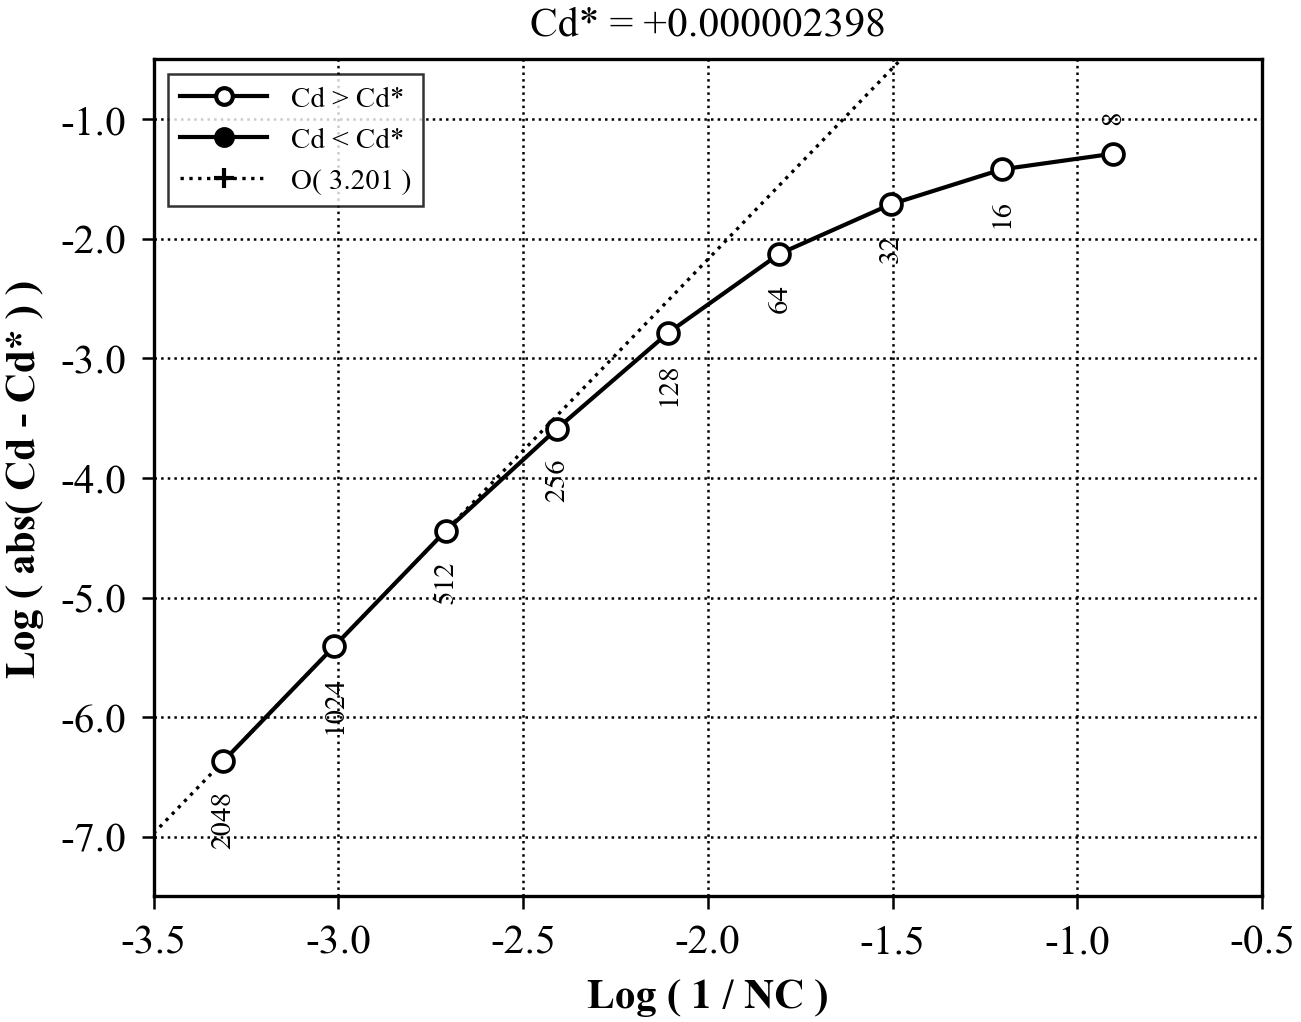
\includegraphics[width=\linewidth]{gc_M05HK_cd_a0.png}
    \caption{Drag, $\alpha=0^\circ$}
  \end{subfigure}\hspace{0.04\linewidth}
  \begin{subfigure}{0.40\linewidth}
    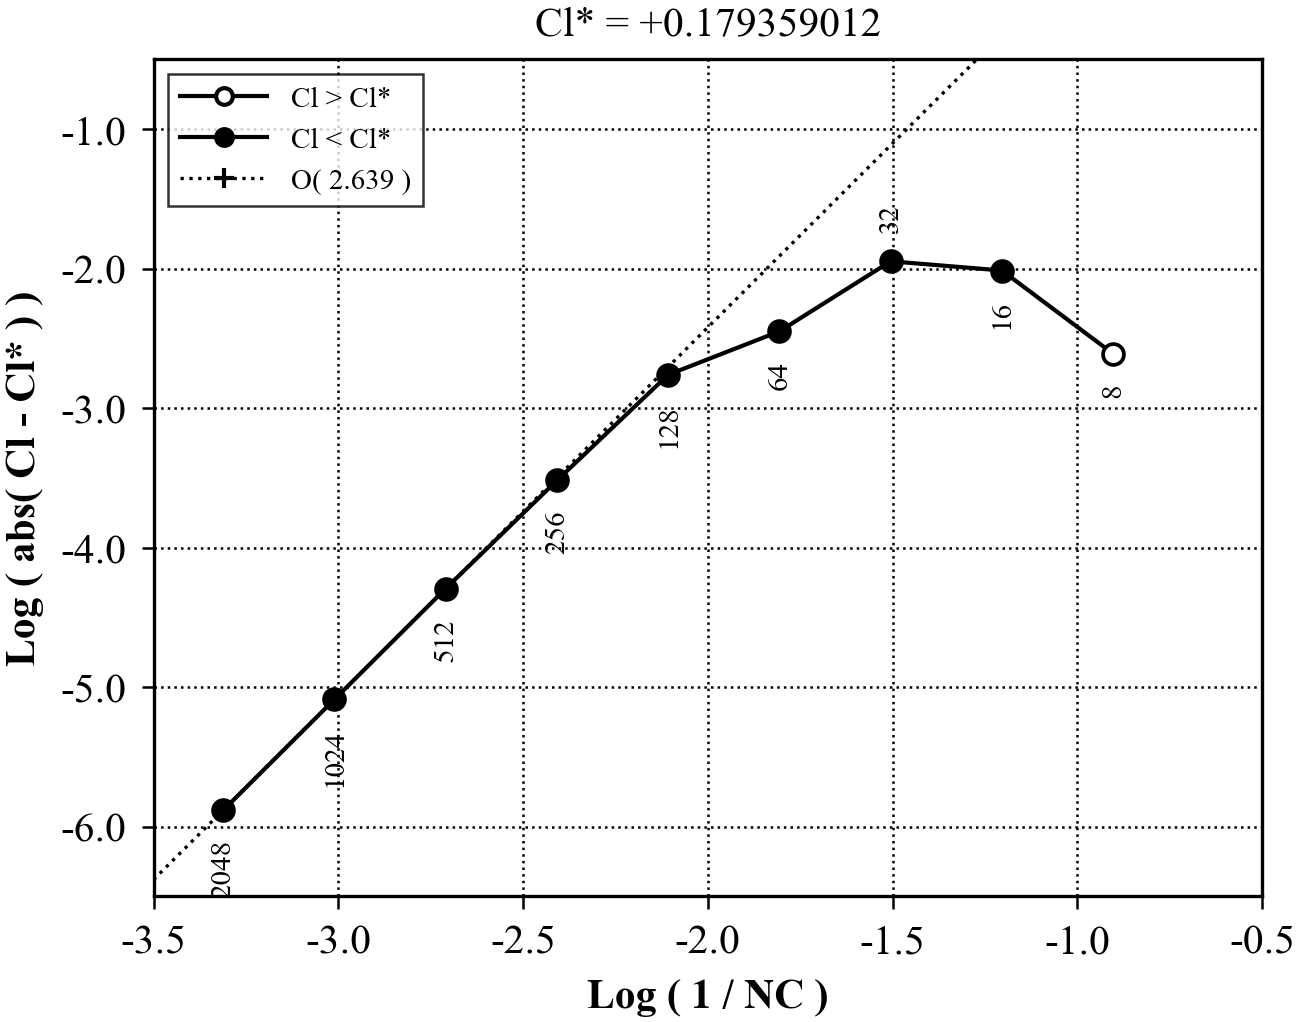
\includegraphics[width=\linewidth]{gc_M05HK_cl_a125.png}
    \caption{Lift, $\alpha=1.25^\circ$}
  \end{subfigure}\\[4pt]
  \begin{subfigure}{0.40\linewidth}
    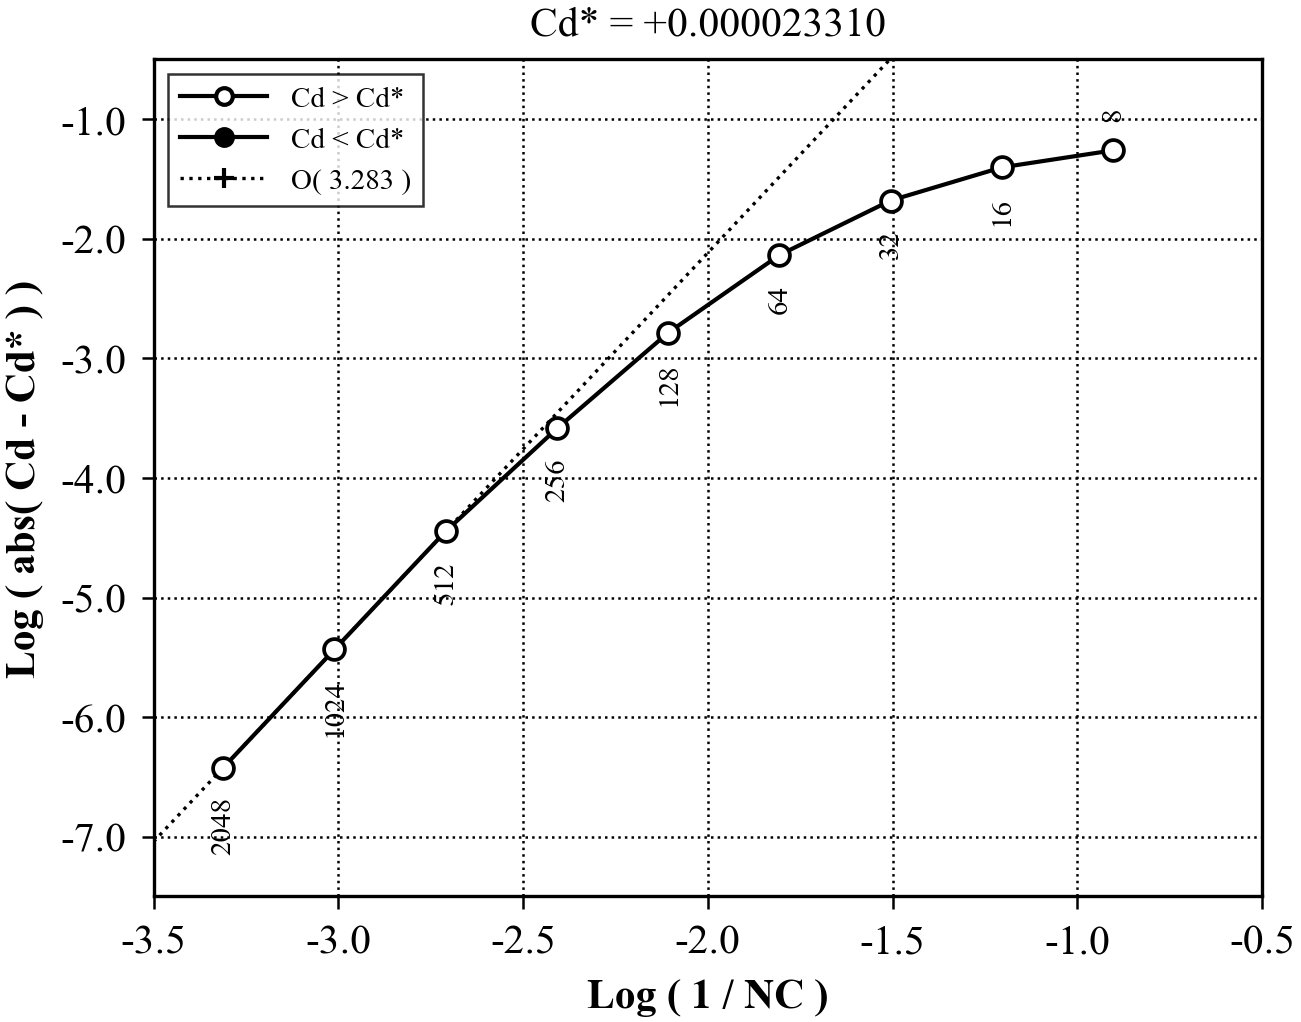
\includegraphics[width=\linewidth]{gc_M05HK_cd_a125.png}
    \caption{Drag, $\alpha=1.25^\circ$}
  \end{subfigure}\hspace{0.04\linewidth}
  \begin{subfigure}{0.40\linewidth}
    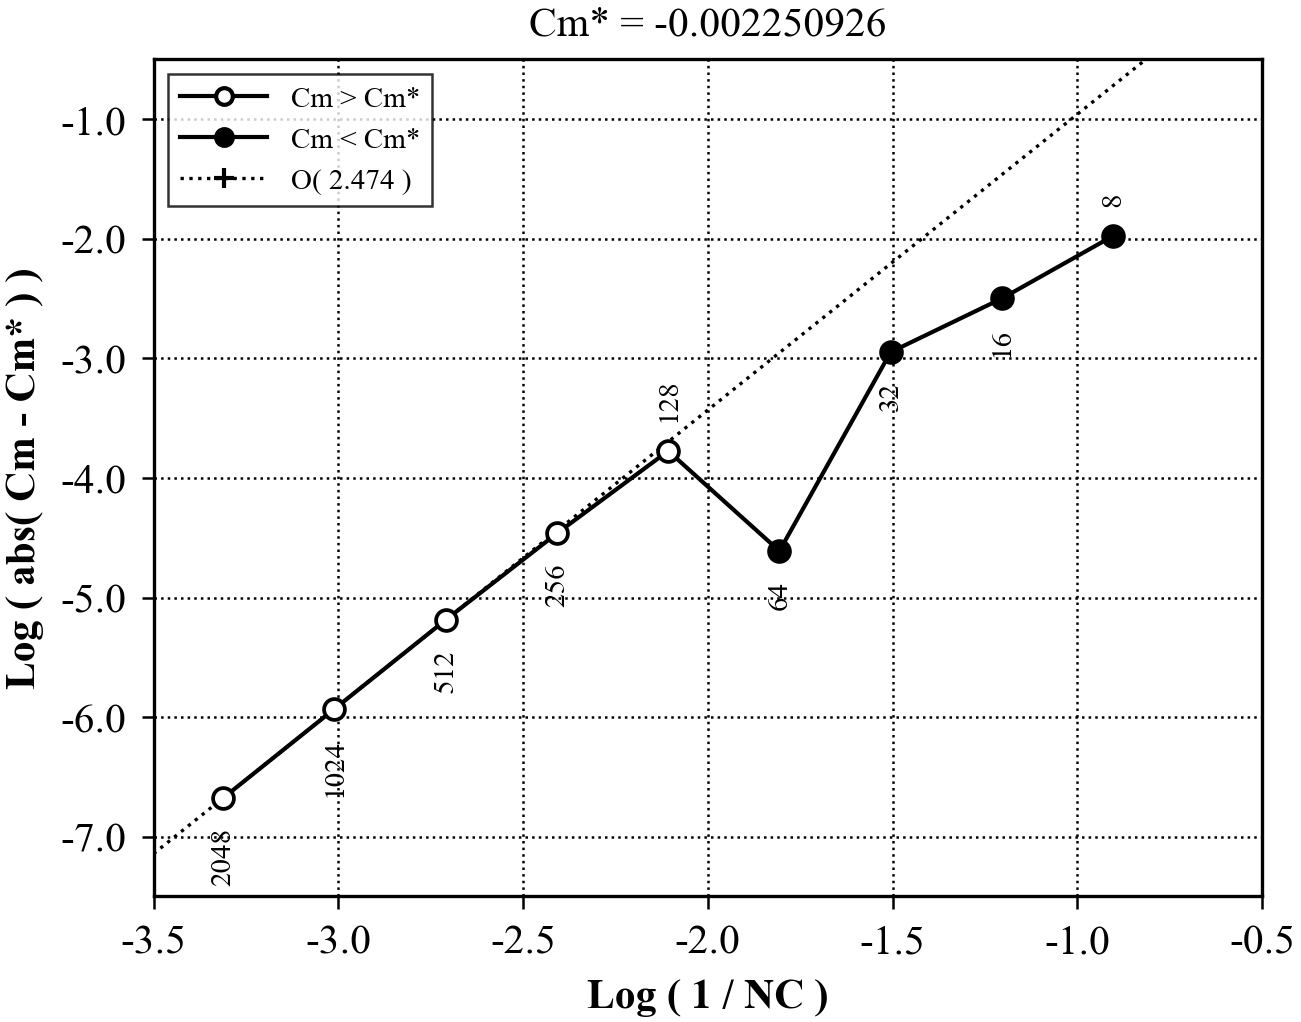
\includegraphics[width=\linewidth]{gc_M05HK_cm_a125.png}
    \caption{Moment, $\alpha=1.25^\circ$}
  \end{subfigure}
  \caption{Grid convergence of the force coefficients, $M_\infty=0.5$}
  \label{fig:gc_errors}
\end{figure}

% Part 4: subsonic, transonic and supersonic solutions
\section{Subsonic, transonic and supersonic flows}\label{sec:flows}

All results of this section use the Hemker--Koren limiter, and the flow fields and pressure
distributions come from the finest grid ($NC=2048$).

\subsection{Subsonic flow, \texorpdfstring{$M_\infty=0.5$}{M = 0.5}}

The force coefficients are those of Table~\ref{tab:gc_forces}. The flow has no shock at either
incidence (Figures~\ref{fig:mach_M05_a0} and~\ref{fig:mach_M05_a125}), and the pressure recovers
smoothly to the trailing edge (Figures~\ref{fig:cp_M05_a0} and~\ref{fig:cp_M05_a125}).
The convergence of the residual and of the force coefficients at $\alpha=1.25^\circ$ is
monitored in Appendix~\ref{app:conv}.

\begin{figure}[H]
  \centering
  \begin{minipage}[t]{0.42\linewidth}
    \centering
    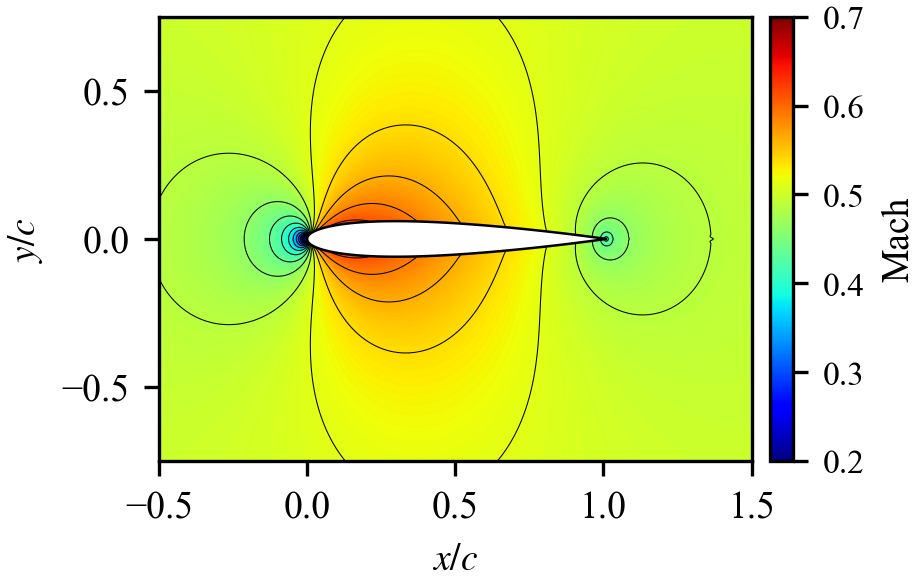
\includegraphics[width=\linewidth]{mach_M05_a0.png}
    \caption{Mach number, $M_\infty=0.5$, $\alpha=0^\circ$}
    \label{fig:mach_M05_a0}
  \end{minipage}\hspace{0.04\linewidth}
  \begin{minipage}[t]{0.42\linewidth}
    \centering
    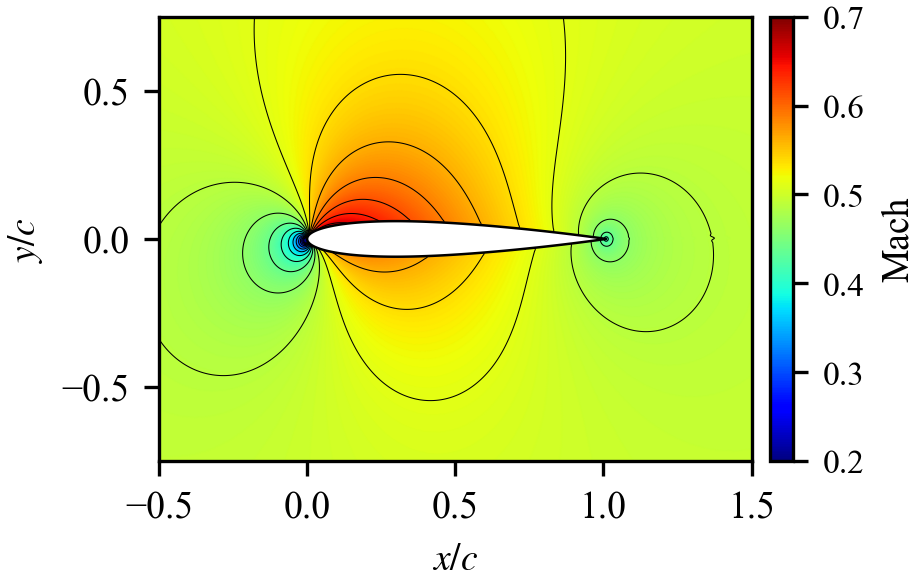
\includegraphics[width=\linewidth]{mach_M05_a125.png}
    \caption{Mach number, $M_\infty=0.5$, $\alpha=1.25^\circ$}
    \label{fig:mach_M05_a125}
  \end{minipage}
\end{figure}

\begin{figure}[H]
  \centering
  \begin{minipage}[t]{0.42\linewidth}
    \centering
    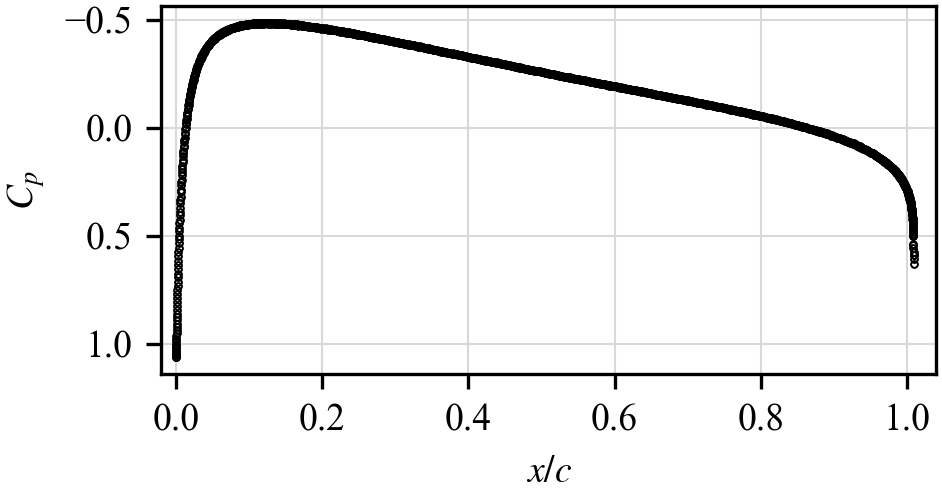
\includegraphics[width=\linewidth]{cp_M05_a0.png}
    \caption{Pressure coefficient, $M_\infty=0.5$, $\alpha=0^\circ$}
    \label{fig:cp_M05_a0}
  \end{minipage}\hspace{0.04\linewidth}
  \begin{minipage}[t]{0.42\linewidth}
    \centering
    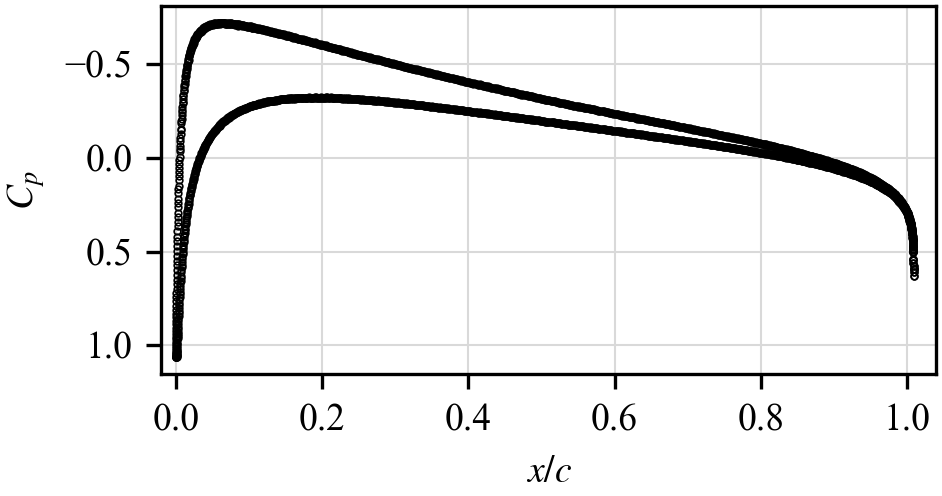
\includegraphics[width=\linewidth]{cp_M05_a125.png}
    \caption{Pressure coefficient, $M_\infty=0.5$, $\alpha=1.25^\circ$}
    \label{fig:cp_M05_a125}
  \end{minipage}
\end{figure}

\subsection{Transonic flow, \texorpdfstring{$M_\infty=0.8$}{M = 0.8}}

Table~\ref{tab:forces_M08} gives the force coefficients. At $M_\infty=0.8$ the flow accelerating
around the thick part of the airfoil becomes supersonic, and the pocket cannot recompress
smoothly to the subsonic pressure of the trailing edge: it ends in a shock, which produces a
wave drag. At $\alpha=0^\circ$ the two surfaces carry the same pocket and shock, so there is no
lift (Figures~\ref{fig:mach_M08_a0} and~\ref{fig:cp_M08_a0}). At $\alpha=1.25^\circ$ the flow
accelerates more over the upper surface, whose shock becomes stronger and moves towards the trailing edge, and less over
the lower surface, whose shock weakens and moves towards the leading edge (Figures~\ref{fig:mach_M08_a125}
and~\ref{fig:cp_M08_a125}); this asymmetry produces the lift and increases the drag. The results
of both subsonic and transonic conditions with the Van Albada limiter are given in
Appendix~\ref{app:va_forces}.
The convergence of the residual and of the force coefficients at $\alpha=1.25^\circ$ is
monitored in Appendix~\ref{app:conv}.

\begin{table}[H]
\centering
\caption{Force coefficients and run times, $M_\infty=0.8$}
\label{tab:forces_M08}
\footnotesize
\setlength{\tabcolsep}{4pt}
\renewcommand{\arraystretch}{1.0}
\begin{tabular}{@{}rrcrcccr@{}}
\toprule
\multicolumn{2}{c}{Mesh} & \multicolumn{2}{c}{$\alpha=0^\circ$} & \multicolumn{4}{c}{$\alpha=1.25^\circ$} \\
\cmidrule(lr){1-2}\cmidrule(lr){3-4}\cmidrule(l){5-8}
$NC$ & $NC^2$ & $C_D$ & $t$ (s) & $C_L$ & $C_D$ & $C_M$ & $t$ (s) \\
\midrule
8 & 64 & $+0.065824993$ & 0.01 & $+0.244246812$ & $+0.072158167$ & $-0.041220036$ & 0.03 \\
16 & 256 & $+0.045091296$ & 0.02 & $+0.332558420$ & $+0.057690342$ & $-0.031002772$ & 0.04 \\
32 & 1{,}024 & $+0.021527162$ & 0.08 & $+0.348908707$ & $+0.036465003$ & $-0.037886563$ & 0.12 \\
64 & 4{,}096 & $+0.012911884$ & 0.50 & $+0.363799762$ & $+0.027699576$ & $-0.041826574$ & 0.51 \\
128 & 16{,}384 & $+0.009255523$ & 4.58 & $+0.360274490$ & $+0.023806424$ & $-0.040705500$ & 3.83 \\
256 & 65{,}536 & $+0.008488427$ & 51.2 & $+0.357186186$ & $+0.022885125$ & $-0.039696950$ & 62.2 \\
512 & 262{,}144 & $+0.008366450$ & 191.3 & $+0.354755929$ & $+0.022627704$ & $-0.038940166$ & 329.7 \\
1{,}024 & 1{,}048{,}576 & $+0.008346639$ & 1{,}787 & $+0.353478031$ & $+0.022540341$ & $-0.038552711$ & 3{,}517 \\
2{,}048 & 4{,}194{,}304 & $+0.008347370$ & 40{,}205 & $+0.352355497$ & $+0.022480045$ & $-0.038222514$ & 100{,}498 \\
\bottomrule
\end{tabular}
\end{table}

\begin{figure}[H]
  \centering
  \begin{minipage}[t]{0.42\linewidth}
    \centering
    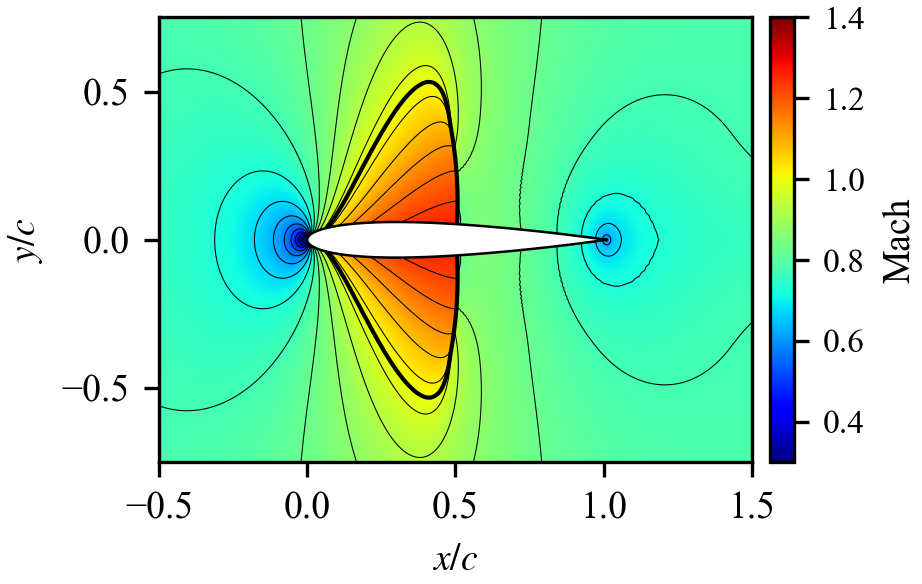
\includegraphics[width=\linewidth]{mach_M08_a0.png}
    \caption{Mach number, $M_\infty=0.8$, $\alpha=0^\circ$}
    \label{fig:mach_M08_a0}
  \end{minipage}\hspace{0.04\linewidth}
  \begin{minipage}[t]{0.42\linewidth}
    \centering
    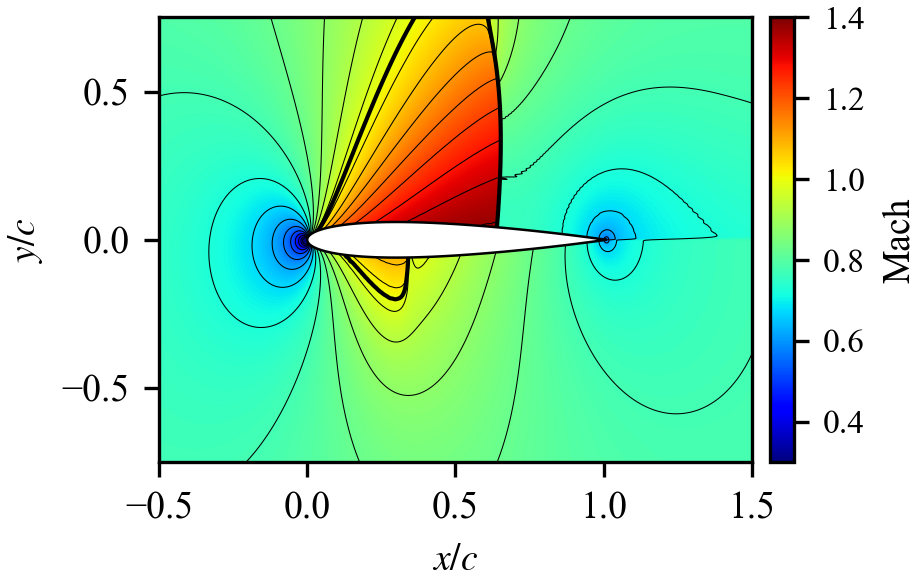
\includegraphics[width=\linewidth]{mach_M08_a125.png}
    \caption{Mach number, $M_\infty=0.8$, $\alpha=1.25^\circ$}
    \label{fig:mach_M08_a125}
  \end{minipage}
\end{figure}

\begin{figure}[H]
  \centering
  \begin{minipage}[t]{0.42\linewidth}
    \centering
    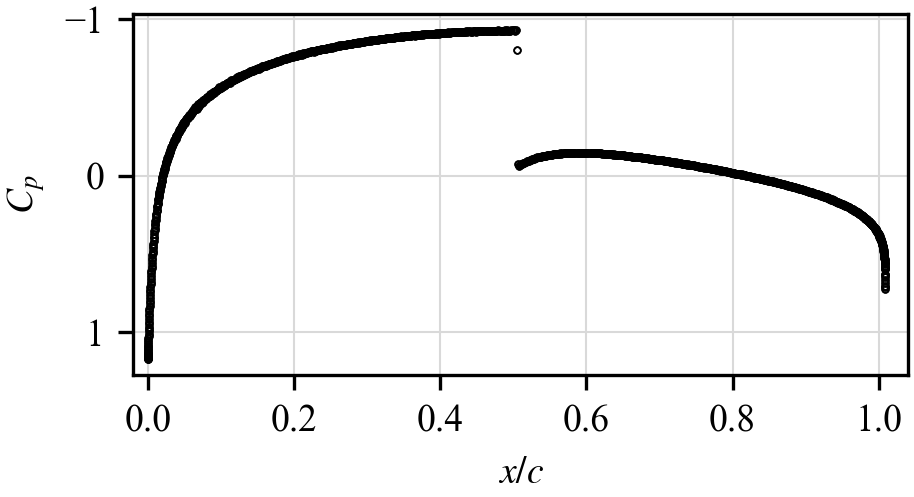
\includegraphics[width=\linewidth]{cp_M08_a0.png}
    \caption{Pressure coefficient, $M_\infty=0.8$, $\alpha=0^\circ$}
    \label{fig:cp_M08_a0}
  \end{minipage}\hspace{0.04\linewidth}
  \begin{minipage}[t]{0.42\linewidth}
    \centering
    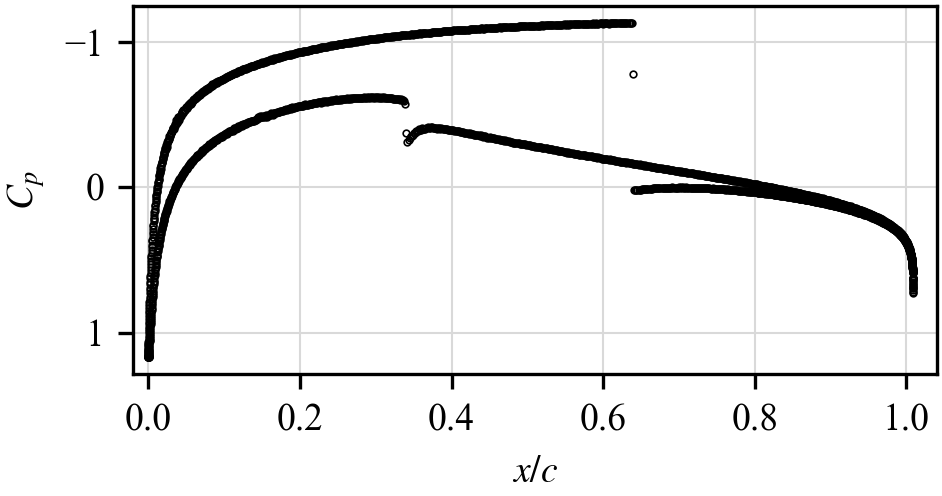
\includegraphics[width=\linewidth]{cp_M08_a125.png}
    \caption{Pressure coefficient, $M_\infty=0.8$, $\alpha=1.25^\circ$}
    \label{fig:cp_M08_a125}
  \end{minipage}
\end{figure}

\subsection{Supersonic flow, \texorpdfstring{$M_\infty=1.25$}{M = 1.25}}

Table~\ref{tab:forces_M125} gives the force coefficients. A detached shock stands ahead of
the leading edge (Figures~\ref{fig:mach_M125_a0} and~\ref{fig:mach_M125_a125}); behind it the flow
near the stagnation point is subsonic, then accelerates back to supersonic speed and expands over
the whole airfoil (Figures~\ref{fig:cp_M125_a0} and~\ref{fig:cp_M125_a125}), before leaving the
trailing edge through two oblique shocks.
The convergence of the residual and of the force coefficients at $\alpha=1.25^\circ$ is
monitored in Appendix~\ref{app:conv}.

\begin{table}[H]
\centering
\caption{Force coefficients and run times, $M_\infty=1.25$}
\label{tab:forces_M125}
\footnotesize
\setlength{\tabcolsep}{4pt}
\renewcommand{\arraystretch}{1.0}
\begin{tabular}{@{}rrcrcccr@{}}
\toprule
\multicolumn{2}{c}{Mesh} & \multicolumn{2}{c}{$\alpha=0^\circ$} & \multicolumn{4}{c}{$\alpha=1.25^\circ$} \\
\cmidrule(lr){1-2}\cmidrule(lr){3-4}\cmidrule(l){5-8}
$NC$ & $NC^2$ & $C_D$ & $t$ (s) & $C_L$ & $C_D$ & $C_M$ & $t$ (s) \\
\midrule
8 & 64 & $+0.130562597$ & 0.01 & $+0.084945499$ & $+0.132402161$ & $-0.019783278$ & 0.01 \\
16 & 256 & $+0.116682869$ & 0.02 & $+0.083371056$ & $+0.118525995$ & $-0.018560785$ & 0.03 \\
32 & 1{,}024 & $+0.105765151$ & 0.09 & $+0.087662364$ & $+0.107626573$ & $-0.019166287$ & 0.08 \\
64 & 4{,}096 & $+0.099126369$ & 36.4 & $+0.088901685$ & $+0.100905013$ & $-0.019067131$ & 0.96 \\
128 & 16{,}384 & $+0.096696283$ & 2.98 & $+0.089238236$ & $+0.098475203$ & $-0.018972964$ & 5.28 \\
256 & 65{,}536 & $+0.096198275$ & 60.9 & $+0.089355199$ & $+0.097980760$ & $-0.018946919$ & 24.8 \\
512 & 262{,}144 & $+0.096143957$ & 453.8 & $+0.089370416$ & $+0.097925737$ & $-0.018932209$ & 6{,}607 \\
1{,}024 & 1{,}048{,}576 & $+0.096144021$ & 10{,}259 & $+0.089360688$ & $+0.097926946$ & $-0.018922425$ & 20{,}357 \\
2{,}048 & 4{,}194{,}304 & $+0.096148939$ & 68{,}598 & $+0.089355985$ & $+0.097931002$ & $-0.018920155$ & 49{,}712 \\
\bottomrule
\end{tabular}
\end{table}

\begin{figure}[H]
  \centering
  \begin{minipage}[t]{0.42\linewidth}
    \centering
    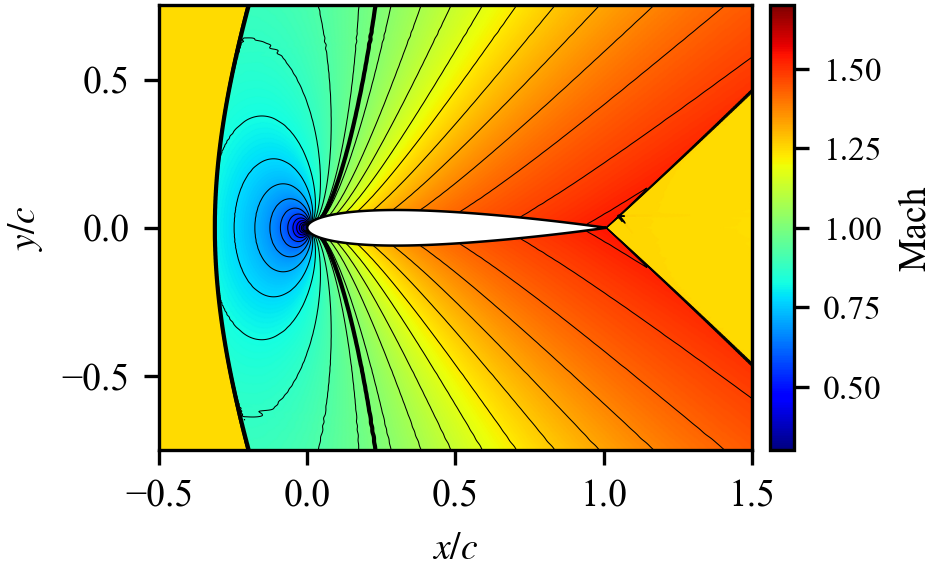
\includegraphics[width=\linewidth]{mach_M125_a0.png}
    \caption{Mach number, $M_\infty=1.25$, $\alpha=0^\circ$}
    \label{fig:mach_M125_a0}
  \end{minipage}\hspace{0.04\linewidth}
  \begin{minipage}[t]{0.42\linewidth}
    \centering
    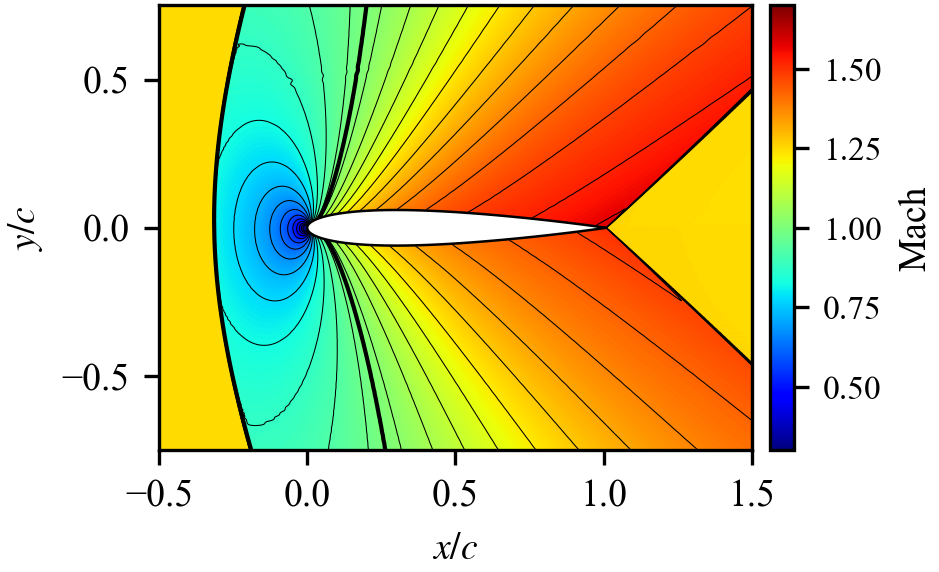
\includegraphics[width=\linewidth]{mach_M125_a125.png}
    \caption{Mach number, $M_\infty=1.25$, $\alpha=1.25^\circ$}
    \label{fig:mach_M125_a125}
  \end{minipage}
\end{figure}

\begin{figure}[H]
  \centering
  \begin{minipage}[t]{0.42\linewidth}
    \centering
    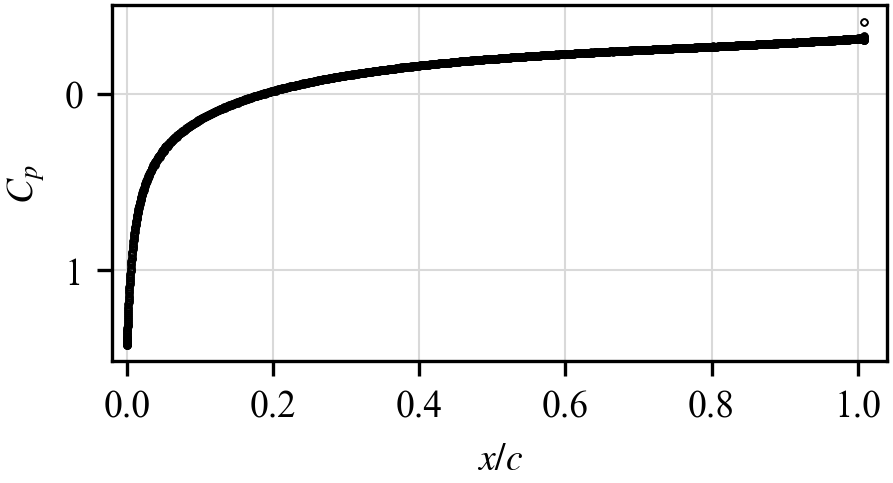
\includegraphics[width=\linewidth]{cp_M125_a0.png}
    \caption{Pressure coefficient, $M_\infty=1.25$, $\alpha=0^\circ$}
    \label{fig:cp_M125_a0}
  \end{minipage}\hspace{0.04\linewidth}
  \begin{minipage}[t]{0.42\linewidth}
    \centering
    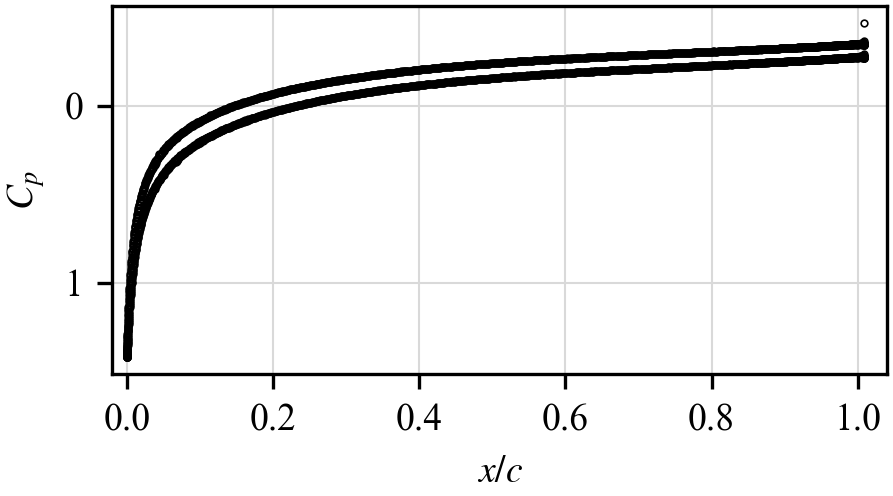
\includegraphics[width=\linewidth]{cp_M125_a125.png}
    \caption{Pressure coefficient, $M_\infty=1.25$, $\alpha=1.25^\circ$}
    \label{fig:cp_M125_a125}
  \end{minipage}
\end{figure}

% Part 5: fixed lift coefficient, M 0.8, CL 0.4
\section{Fixed lift coefficient}\label{sec:fixedcl}

The transonic case is now computed at a prescribed lift, $C_{L,t}=0.4$ at $M_\infty=0.8$, with
the Hemker--Koren limiter. The angle of attack becomes an unknown, found during the flow
iterations by a secant method on $C_L(\alpha)$; the current $\alpha$ sets the free-stream
velocity $\mathbf{V}_a$ of the far-field condition~\eqref{eq:farfield} and the lift and drag
directions. The algorithm and its settings are given in Appendix~\ref{app:fixedcl}.

Table~\ref{tab:fixedcl} gives the angle of attack and the force coefficients obtained at
$C_{L,t}$ on the grids from $NC=8$ to 1024, and Figures~\ref{fig:mach_M08_CL04}
and~\ref{fig:cp_M08_CL04} show the Mach number and the surface pressure on the finest grid.
During the iterations the residual and the angle of attack oscillate, each change of $\alpha$
making the residual jump, until $C_L$ settles on the target and the flow converges.
The convergence of the residual and of the force coefficients is monitored in
Appendix~\ref{app:conv}.

\begin{table}[H]
\centering
\caption{Fixed lift coefficient, $M_\infty=0.8$, $C_L=0.4$}
\label{tab:fixedcl}
\footnotesize
\setlength{\tabcolsep}{4pt}
\renewcommand{\arraystretch}{1.0}
\begin{tabular}{@{}rrcccr@{}}
\toprule
$NC$ & $NC^2$ & $\alpha$ (deg) & $C_D$ & $C_M$ & $t$ (s) \\
\midrule
8 & 64 & $2.062237$ & $+0.082941421$ & $-0.068690715$ & 0.01 \\
16 & 256 & $1.432473$ & $+0.063135968$ & $-0.043537501$ & 0.06 \\
32 & 1{,}024 & $1.448488$ & $+0.040879185$ & $-0.045954929$ & 0.12 \\
64 & 4{,}096 & $1.382307$ & $+0.030665030$ & $-0.047536968$ & 0.80 \\
128 & 16{,}384 & $1.391442$ & $+0.027031873$ & $-0.047097758$ & 7.99 \\
256 & 65{,}536 & $1.401343$ & $+0.026342910$ & $-0.046588900$ & 99.1 \\
512 & 262{,}144 & $1.412651$ & $+0.026296789$ & $-0.046101642$ & 963.1 \\
1{,}024 & 1{,}048{,}576 & $1.417252$ & $+0.026311342$ & $-0.045912467$ & 9{,}890 \\
\bottomrule
\end{tabular}
\end{table}

\begin{figure}[H]
  \centering
  \begin{minipage}[t]{0.42\linewidth}
    \centering
    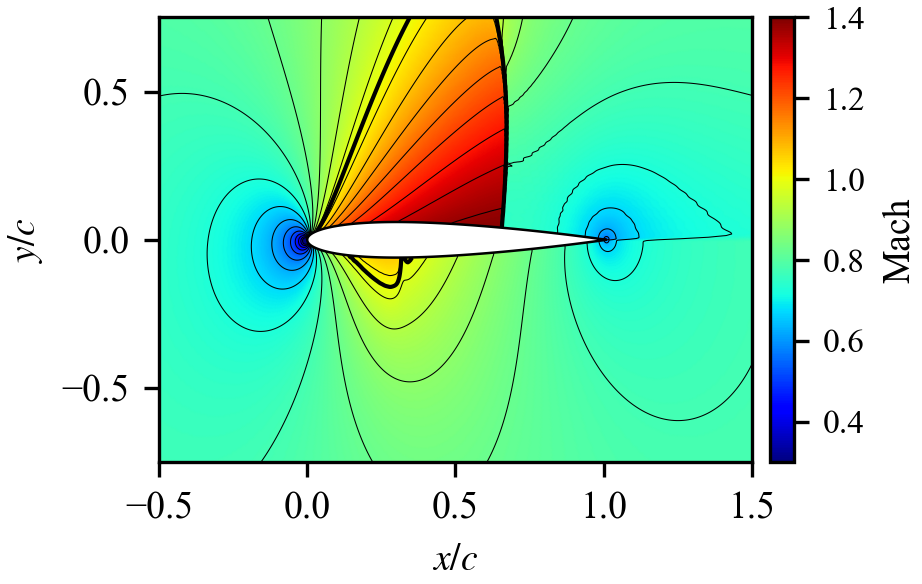
\includegraphics[width=\linewidth]{mach_M08_CL04.png}
    \caption{Mach number, $M_\infty=0.8$, $C_L=0.4$}
    \label{fig:mach_M08_CL04}
  \end{minipage}\hspace{0.04\linewidth}
  \begin{minipage}[t]{0.42\linewidth}
    \centering
    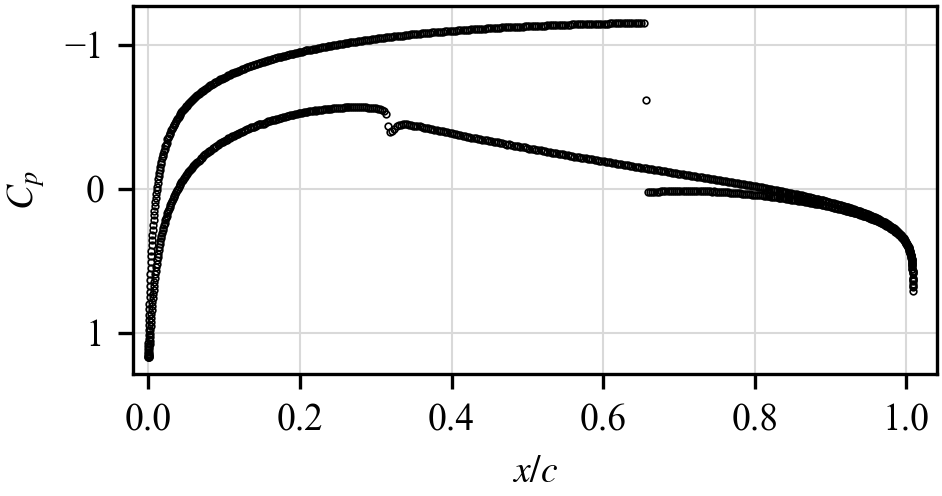
\includegraphics[width=\linewidth]{cp_M08_CL04.png}
    \caption{Pressure coefficient, $M_\infty=0.8$, $C_L=0.4$}
    \label{fig:cp_M08_CL04}
  \end{minipage}
\end{figure}

\vfill
\noindent{\footnotesize\textit{Note:} This work has been realised with the help of AI, notably to
generate parts of the code such as the tests and the post-processing, as well as for debugging,
commenting the code and correcting the report.\par}

\clearpage
\phantomsection
\addcontentsline{toc}{section}{References}
\begin{thebibliography}{99}
\bibitem{vj2010} J.~C. Vassberg and A.~Jameson, ``In pursuit of grid convergence for two-dimensional Euler solutions,''
  \emph{Journal of Aircraft}, 47(4):1152--1166, 2010.
\bibitem{blazek} J.~Blazek, \emph{Computational Fluid Dynamics: Principles and Applications}, 3rd ed.,
  Butterworth-Heinemann, 2015.
\bibitem{venkat1995} V.~Venkatakrishnan, ``Convergence to steady state solutions of the Euler equations on
  unstructured grids with limiters,'' \emph{Journal of Computational Physics}, 118(1):120--130, 1995.
\end{thebibliography}

\appendix

\clearpage
\section{Roe flux}\label{app:roe}

The Roe flux at a face of unit normal $\mathbf{n}=(n_x,n_y)$ splits into the
average of the physical fluxes and an upwind dissipation:
\begin{equation}
  \widehat{\mathbf{F}}=\tfrac12\left[\mathbf{F}_c(\mathbf{W}_R)+\mathbf{F}_c(\mathbf{W}_L)
  -|\tilde{\mathbf{A}}|\,(\mathbf{W}_R-\mathbf{W}_L)\right],
  \qquad
  \mathbf{F}_c=\begin{bmatrix}\rho V\\ \rho uV+n_xp\\ \rho vV+n_yp\\ \rho HV\end{bmatrix},
  \label{eq:roe}
\end{equation}
with $V=un_x+vn_y$ and $H=E+p/\rho$. The quantities used by Algorithm~\ref{alg:roe} are:
\begin{itemize}
  \item the Roe-averaged state, with $\tilde q^2=\tilde u^2+\tilde v^2$ and $\tilde V=\tilde un_x+\tilde vn_y$,
  \begin{equation}
    \tilde\rho=\sqrt{\rho_L\rho_R},\qquad
    \tilde\phi=\frac{\phi_L\sqrt{\rho_L}+\phi_R\sqrt{\rho_R}}{\sqrt{\rho_L}+\sqrt{\rho_R}}\ \ (\phi=u,v,H),\qquad
    \tilde c=\sqrt{(\gamma-1)\left(\tilde H-\tfrac12\tilde q^2\right)};
    \label{eq:roeavg}
  \end{equation}
  \item Harten's entropy correction, applied to each eigenvalue
  $\lambda\in\{\tilde V-\tilde c,\,\tilde V,\,\tilde V+\tilde c\}$ with $\delta=\tilde c/10$,
  \begin{equation}
    |\lambda|_\delta=
    \begin{cases}
      |\lambda|, & |\lambda|\ge\delta,\\[2pt]
      \dfrac{\lambda^2+\delta^2}{2\delta}, & |\lambda|<\delta;
    \end{cases}
    \label{eq:harten}
  \end{equation}
  \item the acoustic waves (1, 5) and the entropy and shear waves (2, 3, 4), with
  $\Delta(\cdot)=(\cdot)_R-(\cdot)_L$,
  \begin{equation}
    |\Delta\mathbf{F}_{1,5}|=|\tilde V\mp\tilde c|_\delta\,\frac{\Delta p\mp\tilde\rho\tilde c\,\Delta V}{2\tilde c^2}
    \begin{bmatrix}1\\ \tilde u\mp\tilde c n_x\\ \tilde v\mp\tilde c n_y\\ \tilde H\mp\tilde c\tilde V\end{bmatrix},
    \label{eq:roeac}
  \end{equation}
  \begin{equation}
    |\Delta\mathbf{F}_{2,3,4}|=|\tilde V|_\delta\left\{\left(\Delta\rho-\frac{\Delta p}{\tilde c^2}\right)
    \begin{bmatrix}1\\ \tilde u\\ \tilde v\\ \tilde q^2/2\end{bmatrix}
    +\tilde\rho\begin{bmatrix}0\\ \Delta u-\Delta V n_x\\ \Delta v-\Delta V n_y\\ \tilde u\Delta u+\tilde v\Delta v-\tilde V\Delta V\end{bmatrix}\right\}.
    \label{eq:roewaves}
  \end{equation}
\end{itemize}

\begin{algorithm}[H]
  \caption{Roe flux at one face}
  \label{alg:roe}
  \begin{algorithmic}[1]
    \REQUIRE reconstructed states $\mathbf{U}_L$, $\mathbf{U}_R$ (Appendix~\ref{app:muscl}), unit normal $\mathbf{n}$
    \STATE compute $H_L$, $H_R$ and the physical fluxes $\mathbf{F}_c(\mathbf{W}_L)$, $\mathbf{F}_c(\mathbf{W}_R)$ of Eq.~\eqref{eq:roe}
    \STATE compute the Roe-averaged state $\tilde\rho$, $\tilde u$, $\tilde v$, $\tilde H$, $\tilde c$, $\tilde V$ with Eq.~\eqref{eq:roeavg}
    \STATE correct $|\tilde V-\tilde c|$, $|\tilde V|$, $|\tilde V+\tilde c|$ with Eq.~\eqref{eq:harten}
    \STATE compute the jumps $\Delta\rho$, $\Delta u$, $\Delta v$, $\Delta p$, $\Delta V$ and the dissipation
           $|\tilde{\mathbf{A}}|\Delta\mathbf{W}=|\Delta\mathbf{F}_1|+|\Delta\mathbf{F}_{2,3,4}|+|\Delta\mathbf{F}_5|$
           with Eqs.~\eqref{eq:roeac}--\eqref{eq:roewaves}
    \STATE $\widehat{\mathbf{F}}\gets\tfrac12\left[\mathbf{F}_c(\mathbf{W}_R)+\mathbf{F}_c(\mathbf{W}_L)-|\tilde{\mathbf{A}}|\Delta\mathbf{W}\right]$
    \ENSURE interface flux $\widehat{\mathbf{F}}$, multiplied by $\Delta S_f$ in Eq.~\eqref{eq:fv}
  \end{algorithmic}
\end{algorithm}

At the wall and far-field faces the flux is $\mathbf{F}_c\!\left(\tfrac12(\mathbf{W}_g+\mathbf{W}_i)\right)$,
with $g$ the ghost and $i$ the interior cell.

\clearpage
\section{MUSCL reconstruction}\label{app:muscl}

The second-order states of each face are reconstructed as follows (Figure~\ref{fig:muscl}):
\begin{itemize}
  \item The reconstruction acts on the primitive variables $\mathbf{U}=(\rho,u,v,p)$, one grid
  direction at a time.
  \item At face $I+\tfrac12$ the left state uses cells $I-1$, $I$, $I+1$, and the right state,
  its mirror image, uses cells $I$, $I+1$, $I+2$:
  \begin{equation}
    \mathbf{U}_L=\mathbf{U}_I+\tfrac12\,\delta(a,b_L),
    \qquad
    \mathbf{U}_R=\mathbf{U}_{I+1}-\tfrac12\,\delta(a,b_R).
    \label{eq:muscl}
  \end{equation}
  \item $a=\mathbf{U}_{I+1}-\mathbf{U}_I$ is the jump across the face;
  $b_L=\mathbf{U}_I-\mathbf{U}_{I-1}$ and $b_R=\mathbf{U}_{I+2}-\mathbf{U}_{I+1}$ are the jumps on
  the far side of each state.
\end{itemize}

\begin{figure}[H]
  \centering
  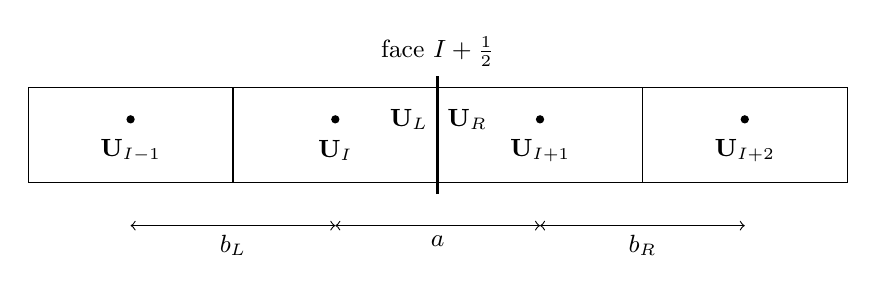
\begin{tikzpicture}[x=2.6cm, y=1cm, font=\small]
    % four cells I-1, I, I+1, I+2
    \foreach \k/\lab in {0/{I-1}, 1/{I}, 2/{I+1}, 3/{I+2}} {
      \draw (\k,0) rectangle (\k+1,1.2);
      \fill (\k+0.5,0.8) circle (1.5pt);
      \node at (\k+0.5,0.4) {$\mathbf{U}_{\lab}$};
    }
    % face I+1/2
    \draw[very thick] (2,-0.15) -- (2,1.35);
    \node[above] at (2,1.35) {face $I+\tfrac12$};
    \node[left]  at (2,0.8) {$\mathbf{U}_L$};
    \node[right] at (2,0.8) {$\mathbf{U}_R$};
    % jumps between cell centres
    \draw[<->] (0.5,-0.55) -- node[below] {$b_L$} (1.5,-0.55);
    \draw[<->] (1.5,-0.55) -- node[below] {$a$} (2.5,-0.55);
    \draw[<->] (2.5,-0.55) -- node[below] {$b_R$} (3.5,-0.55);
  \end{tikzpicture}
  \caption{MUSCL stencil}
  \label{fig:muscl}
\end{figure}

The limited slope $\delta$ is the smooth form of one of two limiters:
\begin{itemize}
  \item Hemker--Koren ($\hat\kappa=1/3$) and Van Albada ($\hat\kappa=0$),
  \begin{equation}
    \delta_{\mathrm{HK}}=\frac{(2a^2+\varepsilon)\,b+(b^2+2\varepsilon)\,a}{2a^2+2b^2-ab+3\varepsilon},
    \qquad
    \delta_{\mathrm{VA}}=\frac{a\,(b^2+\varepsilon)+b\,(a^2+\varepsilon)}{a^2+b^2+2\varepsilon};
    \label{eq:limiters}
  \end{equation}
  \item $\varepsilon=(Kh)^3$ with $h=\sqrt{\Omega}$ the cell size and $K=5$~\cite{venkat1995};
  \item near smooth extrema, where $a$ and $b$ vanish, $\varepsilon$ dominates and the extremum
  is not clipped, while at a shock $a^2=O(1)\gg\varepsilon$ and the limiter acts fully;
  \item for $\varepsilon\to\infty$ the two slopes become the unlimited $\hat\kappa=1/3$ and
  $\hat\kappa=0$ schemes, $(2a+b)/3$ and $(a+b)/2$.
\end{itemize}

\clearpage
\section{Boundary conditions}\label{app:bc}

Two layers of ghost cells close the stencil; across the O-grid cut they are copies of the cells
on the other side. At the slip wall the normal velocity vanishes, $\mathbf{V}\cdot\mathbf{n}=0$.
The ghost state mirrors the velocity of the first cell and extrapolates its pressure linearly
from the first two cells:
\begin{equation}
  \mathbf{V}_g=\mathbf{V}_1-2(\mathbf{V}_1\cdot\mathbf{n})\,\mathbf{n},
  \qquad
  \rho_g=\rho_1,
  \qquad
  p_g=2p_1-p_2 .
  \label{eq:wall}
\end{equation}
The wall-face flux is the physical flux of the averaged state $\tfrac12(\mathbf{W}_g+\mathbf{W}_1)$,
whose normal velocity is zero, so only the pressure term remains,
$\widehat{\mathbf{F}}_w=(0,\,n_xp_w,\,n_yp_w,\,0)^T$.

At the far field the boundary state $\mathbf{W}_b$ follows the characteristics normal to the
boundary. With $a$ the free stream, $d$ the interior cell, $\rho_0$, $c_0$ taken from $d$ and
$\mathbf{n}$ pointing out of the domain, the face is an inflow when $\mathbf{V}_d\cdot\mathbf{n}<0$
and supersonic when $|\mathbf{V}_d\cdot\mathbf{n}|\ge c_0$. A supersonic inflow takes
$\mathbf{W}_b=\mathbf{W}_a$ and a supersonic outflow $\mathbf{W}_b=\mathbf{W}_d$. In subsonic
flow one characteristic leaves the domain at an inflow and one enters it at an outflow:
\begin{equation}
  \begin{aligned}
    &\text{inflow:} &
    p_b&=\tfrac12\left[p_a+p_d-\rho_0c_0\,\mathbf{n}\cdot(\mathbf{V}_a-\mathbf{V}_d)\right], &
    \rho_b&=\rho_a+\frac{p_b-p_a}{c_0^2}, &
    \mathbf{V}_b&=\mathbf{V}_a-\mathbf{n}\,\frac{p_a-p_b}{\rho_0c_0},\\
    &\text{outflow:} &
    p_b&=p_a, &
    \rho_b&=\rho_d+\frac{p_b-p_d}{c_0^2}, &
    \mathbf{V}_b&=\mathbf{V}_d+\mathbf{n}\,\frac{p_d-p_b}{\rho_0c_0}.
  \end{aligned}
  \label{eq:farfield}
\end{equation}
The ghost state is extrapolated through the boundary, $\mathbf{W}_g=2\mathbf{W}_b-\mathbf{W}_d$,
so that the face average is $\mathbf{W}_b$.

\clearpage
\section{Jacobian-free Newton--Krylov solver}\label{app:gmres}

Each implicit step~\eqref{eq:bdf1} solves $\mathbf{A}\,\Delta\mathbf{W}=\mathbf{b}$ with
$\mathbf{A}=\Omega/\Delta t\,\mathbf{I}+\mathbf{J}$, $\mathbf{J}=\partial\mathbf{R}/\partial\mathbf{W}$
and $\mathbf{b}=-\mathbf{R}(\mathbf{W}^n)$, by restarted GMRES, summarized in
Algorithm~\ref{alg:gmres}. Its ingredients are:
\begin{itemize}
  \item \textbf{Jacobian-free products.} $\mathbf{J}$ is never formed; its product with a vector is
  a finite difference of the second-order residual,
  \begin{equation}
    \mathbf{J}\mathbf{v}\approx\frac{\mathbf{R}(\mathbf{W}+\epsilon\mathbf{v})-\mathbf{R}(\mathbf{W})}{\epsilon},
    \qquad
    \epsilon=\frac{\sqrt{\epsilon_{\mathrm{mach}}}\,(1+\|\mathbf{W}\|)}{\|\mathbf{v}\|}.
    \label{eq:jfnk}
  \end{equation}
  \item \textbf{Preconditioner.} $\mathbf{P}^{-1}$ is two block symmetric Gauss--Seidel sweeps
  (forward then backward over the cells, $4\times4$ diagonal blocks) on the first-order upwind
  operator, whose off-diagonal blocks are
  \begin{equation}
    \frac{\partial\widehat{\mathbf{F}}}{\partial\mathbf{W}_L}=\tfrac12\left[\mathbf{A}_c(\mathbf{W}_L)+|\tilde{\mathbf{A}}|\right],
    \qquad
    \frac{\partial\widehat{\mathbf{F}}}{\partial\mathbf{W}_R}=\tfrac12\left[\mathbf{A}_c(\mathbf{W}_R)-|\tilde{\mathbf{A}}|\right],
    \label{eq:jac1}
  \end{equation}
  with $\mathbf{A}_c=\partial\mathbf{F}_c/\partial\mathbf{W}$ and the frozen Roe matrix
  $|\tilde{\mathbf{A}}|$ (same entropy correction as the flux). The derivatives of the wall and
  far-field fluxes with respect to the interior cell are lumped on the diagonal.
  \item \textbf{Notation.} $\mathbf{v}_1,\dots,\mathbf{v}_{j+1}$ are orthonormal basis vectors and
  $\bar{\mathbf{H}}_j$ is the $(j+1)\times j$ matrix of the coefficients $h_{ik}$; $\mathbf{e}_1=(1,0,\dots,0)^T$.
  \item \textbf{Settings.} Relative tolerance $\eta=10^{-3}$ (inexact Newton), restart length
  $m=150$ to $200$, at most 400 to 800 inner iterations per step on the finest grids.
\end{itemize}

\begin{algorithm}[H]
  \caption{Right-preconditioned restarted GMRES$(m)$ for one implicit step}
  \label{alg:gmres}
  \begin{algorithmic}[1]
    \REQUIRE $\mathbf{W}^n$, $\mathbf{b}=-\mathbf{R}(\mathbf{W}^n)$, local time steps $\Delta t_i$
    \STATE $\mathbf{x}_0=\mathbf{0}$ \COMMENT{initial guess of $\Delta\mathbf{W}^n$}
    \REPEAT
      \STATE $\mathbf{r}_0=\mathbf{b}-\mathbf{A}\mathbf{x}_0$, \ $\beta=\|\mathbf{r}_0\|$, \ $\mathbf{v}_1=\mathbf{r}_0/\beta$ \COMMENT{residual and first basis vector}
      \FOR{$j=1$ \TO $m$}
        \STATE $\mathbf{z}_j=\mathbf{P}^{-1}\mathbf{v}_j$ \COMMENT{two block SGS sweeps}
        \STATE $\mathbf{w}=(\Omega/\Delta t)\,\mathbf{z}_j+\mathbf{J}\mathbf{z}_j$ \COMMENT{matrix-free product, Eq.~\eqref{eq:jfnk}}
        \FOR{$i=1$ \TO $j$}
          \STATE $h_{ij}=\mathbf{w}\cdot\mathbf{v}_i$ \COMMENT{component of $\mathbf{w}$ along $\mathbf{v}_i$}
          \STATE $\mathbf{w}=\mathbf{w}-h_{ij}\,\mathbf{v}_i$ \COMMENT{remove it}
        \ENDFOR
        \STATE $h_{j+1,j}=\|\mathbf{w}\|$, \ $\mathbf{v}_{j+1}=\mathbf{w}/h_{j+1,j}$ \COMMENT{new basis vector}
        \STATE $\mathbf{y}_j=\arg\min_{\mathbf{y}}\|\beta\mathbf{e}_1-\bar{\mathbf{H}}_j\mathbf{y}\|$ \COMMENT{small least-squares problem}
        \IF{$\|\beta\mathbf{e}_1-\bar{\mathbf{H}}_j\mathbf{y}_j\|\le\eta\,\|\mathbf{b}\|$}
          \STATE exit the loop \COMMENT{linear residual small enough}
        \ENDIF
      \ENDFOR
      \STATE $\mathbf{x}_0=\mathbf{x}_0+\sum_{k=1}^{j}y_{j,k}\,\mathbf{z}_k$ \COMMENT{update the solution}
    \UNTIL{$\|\mathbf{b}-\mathbf{A}\mathbf{x}_0\|\le\eta\,\|\mathbf{b}\|$ or the iteration limit} \COMMENT{else restart}
    \ENSURE $\Delta\mathbf{W}^n=\mathbf{x}_0$
  \end{algorithmic}
\end{algorithm}

\clearpage
\section{Full-multigrid start}\label{app:fmg}

The FMG start of Section~\ref{sec:implicit} works on grids nested in the fine one:
\begin{itemize}
  \item removing every other grid line of grid $h$ gives grid $2h$, each coarse cell being made
  of four fine cells;
  \item $L=4$ grids are used in total, e.g.\ $257^2\to513^2\to1025^2\to2049^2$ for the finest grid;
  \item every grid is solved with the same implicit scheme (Section~\ref{sec:implicit}); the coarse
  grids only down to a residual drop of $10^{-6}$ or their iteration limit;
  \item the solution is passed to the next finer grid by injection, every fine cell taking the
  value of the coarse cell that contains it,
  \begin{equation}
    \mathbf{W}^{h}_{2i+r,\,2j+s}=\mathbf{W}^{2h}_{i,j},\qquad r,s\in\{0,1\}.
    \label{eq:inject}
  \end{equation}
\end{itemize}

\begin{algorithm}[H]
  \caption{Full-multigrid start}
  \label{alg:fmg}
  \begin{algorithmic}[1]
    \REQUIRE fine grid $G_L$, number of grids $L$
    \STATE build $G_{L-1},\dots,G_1$ by removing every other grid line ($G_1$ coarsest)
    \STATE $\mathbf{W}_1\gets$ free stream on $G_1$
    \FOR{$l=1$ \TO $L-1$}
      \STATE solve on $G_l$ from $\mathbf{W}_l$ with the implicit scheme, down to a drop of $10^{-6}$
      \STATE $\mathbf{W}_{l+1}\gets$ injection of $\mathbf{W}_l$ on $G_{l+1}$, Eq.~\eqref{eq:inject}
    \ENDFOR
    \STATE solve on $G_L$ from $\mathbf{W}_L$ until the convergence criterion of Section~\ref{sec:implicit}
    \ENSURE converged fine-grid solution
  \end{algorithmic}
\end{algorithm}

The coarse grids are cheap (four times fewer cells per level) and remove most of the
low-frequency error, so the fine grid starts with the shocks and the circulation nearly in place
and the CFL ramp~\eqref{eq:ser} reaches large values after a few iterations.

\clearpage
\section{Fixed-lift computation}\label{app:fixedcl}

The angle of attack of Section~\ref{sec:fixedcl} is found by Algorithm~\ref{alg:fixedcl}:
\begin{itemize}
  \item the angle is changed before the flow is fully converged, once the residual has dropped by
  $\delta$ since the jump caused by the previous change, so that the flow and $\alpha$ converge
  together;
  \item with the FMG start (Appendix~\ref{app:fmg}) every coarse grid is also solved at $C_{L,t}$,
  so the fine grid starts from the angle of the coarser one.
\end{itemize}

\begin{algorithm}[H]
  \caption{Fixed-lift computation}
  \label{alg:fixedcl}
  \begin{algorithmic}[1]
    \REQUIRE target $C_{L,t}$, first guess $\alpha$, perturbation $\Delta\alpha_0$, drop $\delta$
    \LOOP
      \STATE one implicit iteration~\eqref{eq:bdf1} at the current $\alpha$
      \IF{$\|R_\rho\|\le\delta\,\max\|R_\rho\|$ since the last change of $\alpha$, and $|C_L-C_{L,t}|>10^{-6}$}
        \IF{first change}
          \STATE $\Delta\alpha\gets\Delta\alpha_0\,\operatorname{sign}(C_{L,t}-C_L)$
        \ELSE
          \STATE $\Delta\alpha\gets(C_{L,t}-C_L)\,(\alpha-\alpha_{old})/(C_L-C_{L,old})$, limited to $\pm2^\circ$
        \ENDIF
        \STATE $\alpha_{old}\gets\alpha$, $C_{L,old}\gets C_L$, $\alpha\gets\alpha+\Delta\alpha$; update $\mathbf{V}_a$
      \ENDIF
      \STATE \textbf{exit} when the residual is converged and $|C_L-C_{L,t}|\le10^{-6}$
    \ENDLOOP
  \end{algorithmic}
\end{algorithm}

\clearpage
\section{Richardson extrapolation}\label{app:richardson}

The order of accuracy of a functional $F$ ($C_L$, $C_D$ or $C_M$) is estimated from three
successive grids:
\begin{itemize}
  \item the coarse ($c$), medium ($m$) and fine ($f$) grids have cell sizes $h_c=2h_m=4h_f$
  (refinement ratio $\omega=2$);
  \item the ratio of the functional changes between the grids is
  \begin{equation}
    R=\frac{F_f-F_m}{F_m-F_c};
    \label{eq:richardson_R}
  \end{equation}
  \item with $F=F^*+Ch^p$, the order $p$ is the root of
  \begin{equation}
    G(p)=(\omega^{2p}-\omega^p)\,R-\omega^p+1=0,
    \qquad
    G'(p)=\ln(\omega^2)\,\omega^{2p}R-\ln(\omega)\,\omega^p(R+1),
    \label{eq:richardson_G}
  \end{equation}
  found by Newton's method, $p^{k+1}=p^k-G(p^k)/G'(p^k)$; for $\omega=2$ the root is also
  $p=-\log_2R$;
  \item the continuum value follows by Richardson extrapolation,
  \begin{equation}
    F^*=F_f+\frac{F_f-F_m}{\omega^p-1};
    \label{eq:richardson_F}
  \end{equation}
  \item a triplet with $R\le0$ is not monotone and gives no order.
\end{itemize}

\clearpage
\section{Grid convergence at \texorpdfstring{$M_\infty=0.5$}{M = 0.5}, Van Albada limiter}\label{app:gc_M05VA}

Table~\ref{tab:gc_M05VA} gives the observed order $p$ and the continuum value $F^*$ of the two finest
triplets (--: not monotone), and Figure~\ref{fig:gc_M05VA} the
convergence of the force coefficients on all grids. In the figures, open symbols mark $F>F^*$
and filled symbols $F<F^*$.

\begin{table}[H]
\centering
\caption{Observed order and continuum value, $M_\infty=0.5$, Van Albada limiter}
\label{tab:gc_M05VA}
\footnotesize
\setlength{\tabcolsep}{4pt}
\renewcommand{\arraystretch}{1.0}
\begin{tabular}{@{}llcccc@{}}
\toprule
 & & \multicolumn{2}{c}{$NC=256$, 512, 1024} & \multicolumn{2}{c}{$NC=512$, 1024, 2048} \\
\cmidrule(lr){3-4}\cmidrule(l){5-6}
$\alpha$ & $F$ & $p$ & $F^*$ & $p$ & $F^*$ \\
\midrule
$0^\circ$ & $C_D$ & 2.70 & $+0.000001022$ & 2.99 & $+0.000002170$ \\
$1.25^\circ$ & $C_L$ & 2.29 & $+0.179371849$ & 2.60 & $+0.179369466$ \\
 & $C_D$ & 2.69 & $+0.000021722$ & 3.02 & $+0.000023030$ \\
 & $C_M$ & 1.95 & $-0.002253884$ & 2.41 & $-0.002253247$ \\
\bottomrule
\end{tabular}
\end{table}

\begin{figure}[H]
  \centering
  \begin{subfigure}{0.48\linewidth}
    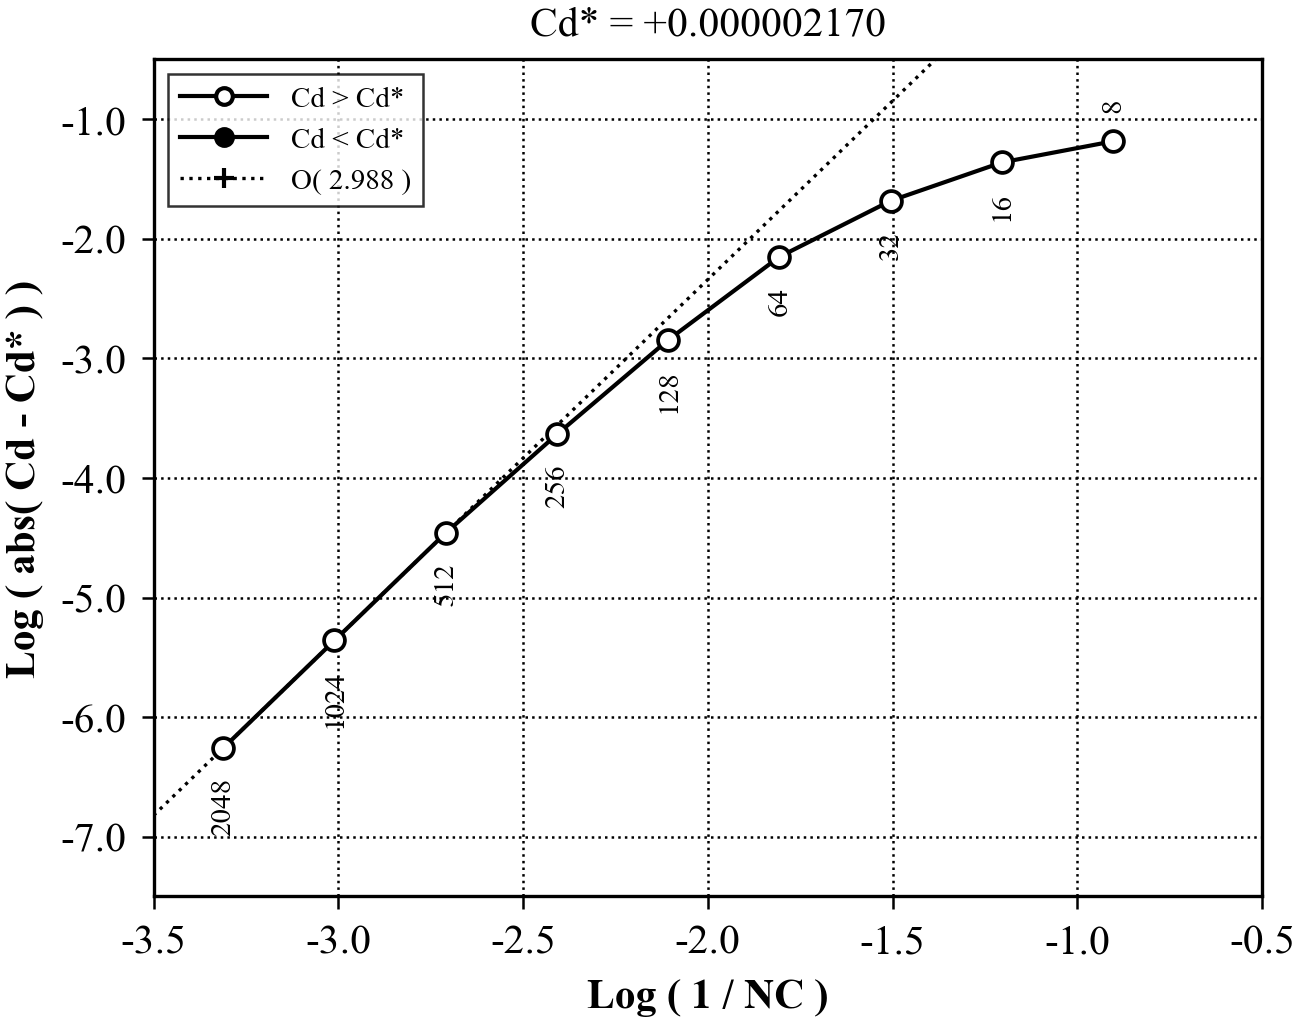
\includegraphics[width=\linewidth]{gc_M05VA_cd_a0.png}
    \caption{Drag, $\alpha=0^\circ$}
  \end{subfigure}\hfill
  \begin{subfigure}{0.48\linewidth}
    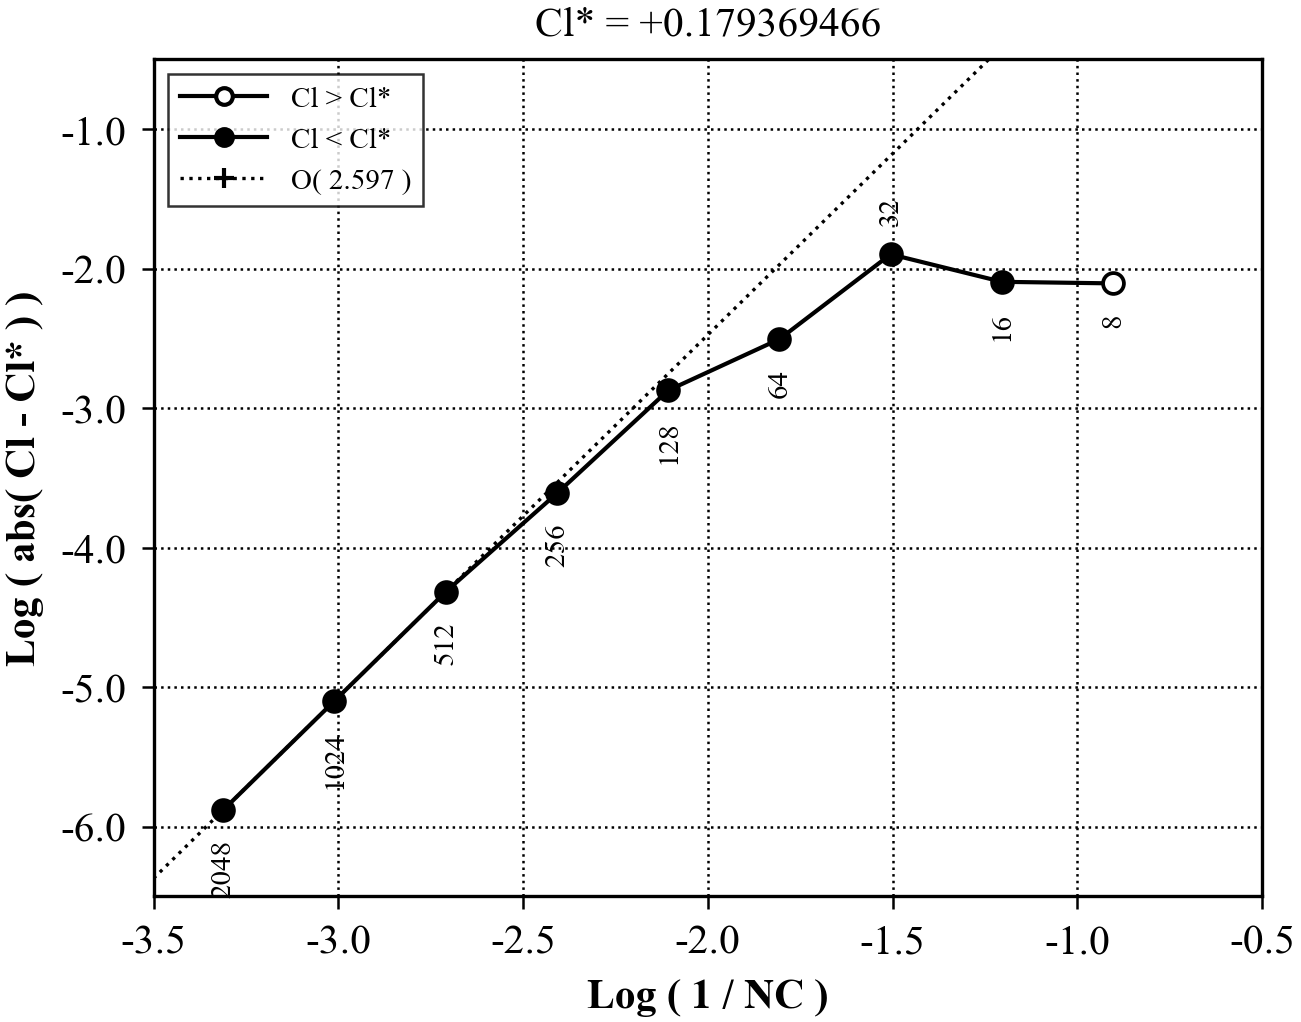
\includegraphics[width=\linewidth]{gc_M05VA_cl_a125.png}
    \caption{Lift, $\alpha=1.25^\circ$}
  \end{subfigure}\\[4pt]
  \begin{subfigure}{0.48\linewidth}
    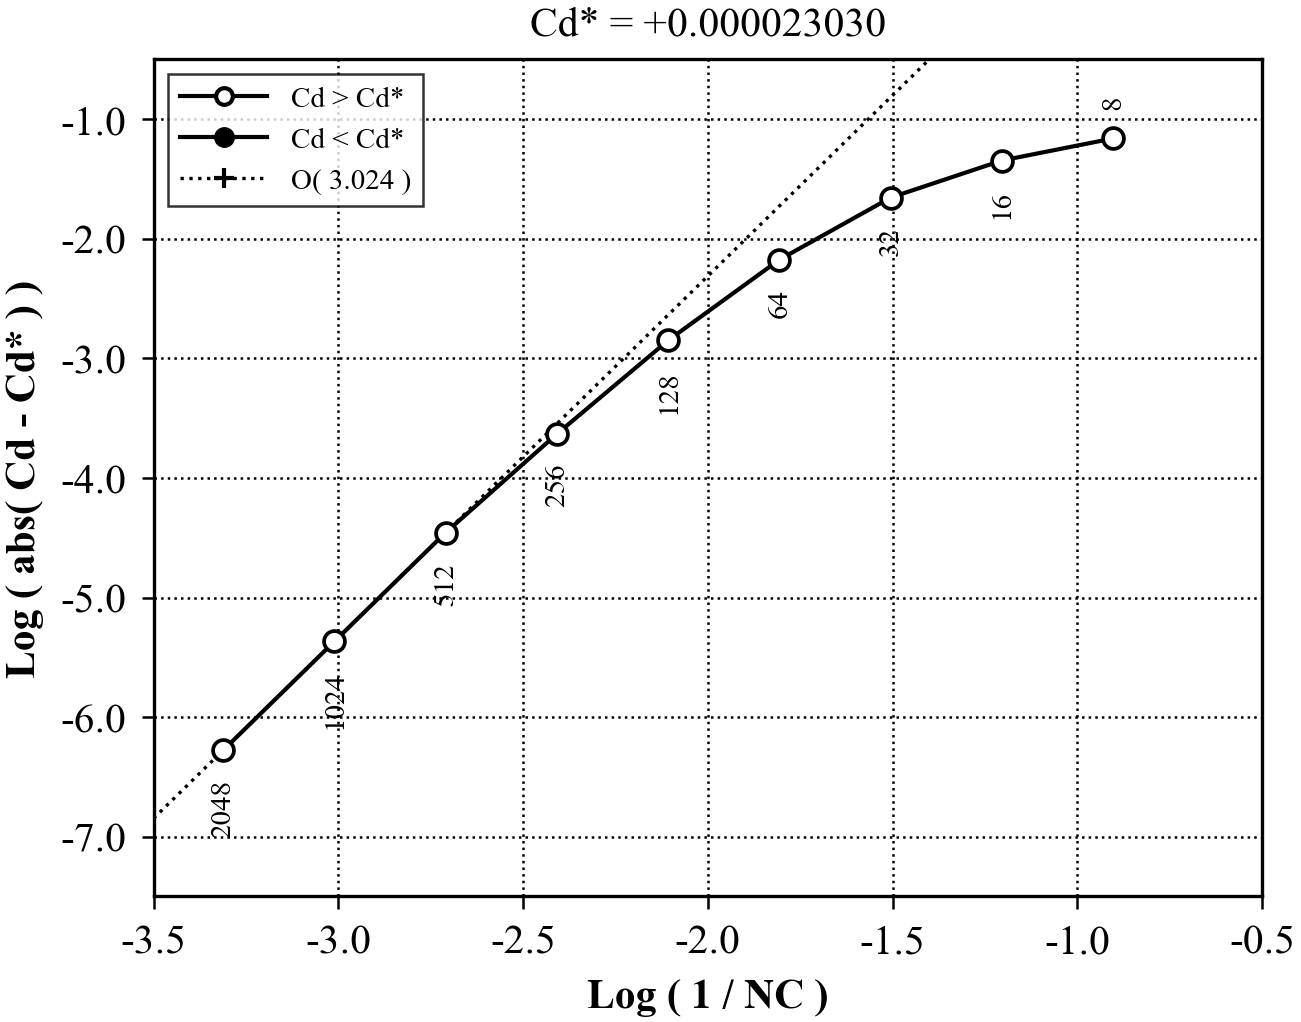
\includegraphics[width=\linewidth]{gc_M05VA_cd_a125.png}
    \caption{Drag, $\alpha=1.25^\circ$}
  \end{subfigure}\hfill
  \begin{subfigure}{0.48\linewidth}
    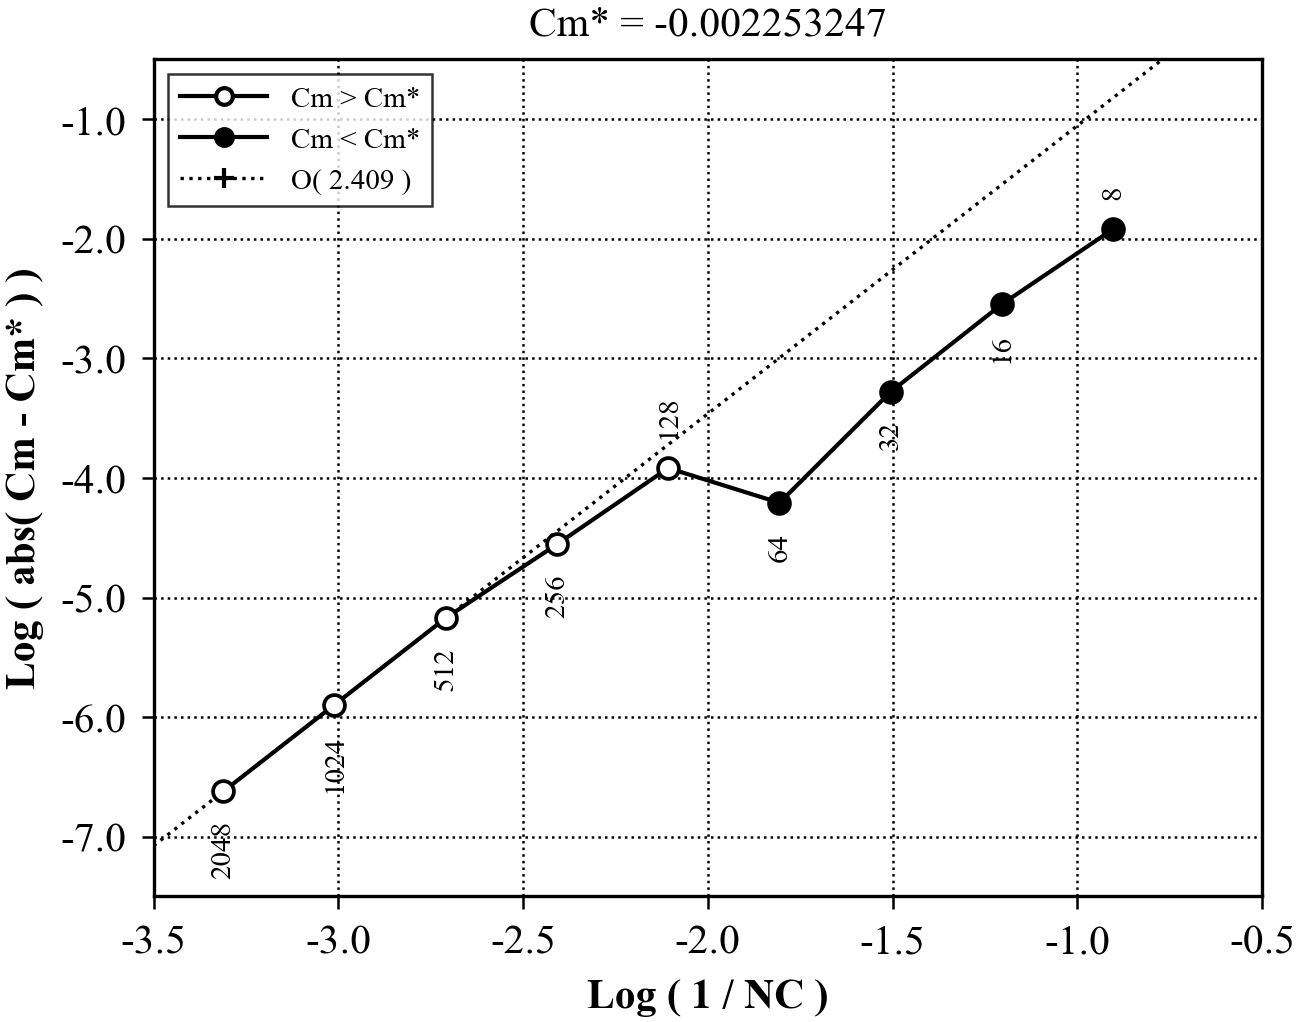
\includegraphics[width=\linewidth]{gc_M05VA_cm_a125.png}
    \caption{Moment, $\alpha=1.25^\circ$}
  \end{subfigure}
  \caption{Grid convergence of the force coefficients, $M_\infty=0.5$, Van Albada limiter}
  \label{fig:gc_M05VA}
\end{figure}

\clearpage
\section{Grid convergence at \texorpdfstring{$M_\infty=0.8$}{M = 0.8}, Hemker--Koren limiter}\label{app:gc_M08HK}

Table~\ref{tab:gc_M08HK} gives the observed order $p$ and the continuum value $F^*$ of the two finest
triplets (--: not monotone), and Figure~\ref{fig:gc_M08HK} the
convergence of the force coefficients on all grids. In the figures, open symbols mark $F>F^*$
and filled symbols $F<F^*$.

\begin{table}[H]
\centering
\caption{Observed order and continuum value, $M_\infty=0.8$}
\label{tab:gc_M08HK}
\footnotesize
\setlength{\tabcolsep}{4pt}
\renewcommand{\arraystretch}{1.0}
\begin{tabular}{@{}llcccc@{}}
\toprule
 & & \multicolumn{2}{c}{$NC=256$, 512, 1024} & \multicolumn{2}{c}{$NC=512$, 1024, 2048} \\
\cmidrule(lr){3-4}\cmidrule(l){5-6}
$\alpha$ & $F$ & $p$ & $F^*$ & $p$ & $F^*$ \\
\midrule
$0^\circ$ & $C_D$ & 2.62 & $+0.008342797$ & -- & -- \\
$1.25^\circ$ & $C_L$ & 0.93 & $+0.352060915$ & 0.19 & $+0.344245016$ \\
 & $C_D$ & 1.56 & $+0.022495459$ & 0.53 & $+0.022345732$ \\
 & $C_M$ & 0.97 & $-0.038146242$ & 0.23 & $-0.036318305$ \\
\bottomrule
\end{tabular}
\end{table}

\begin{figure}[H]
  \centering
  \begin{subfigure}{0.48\linewidth}
    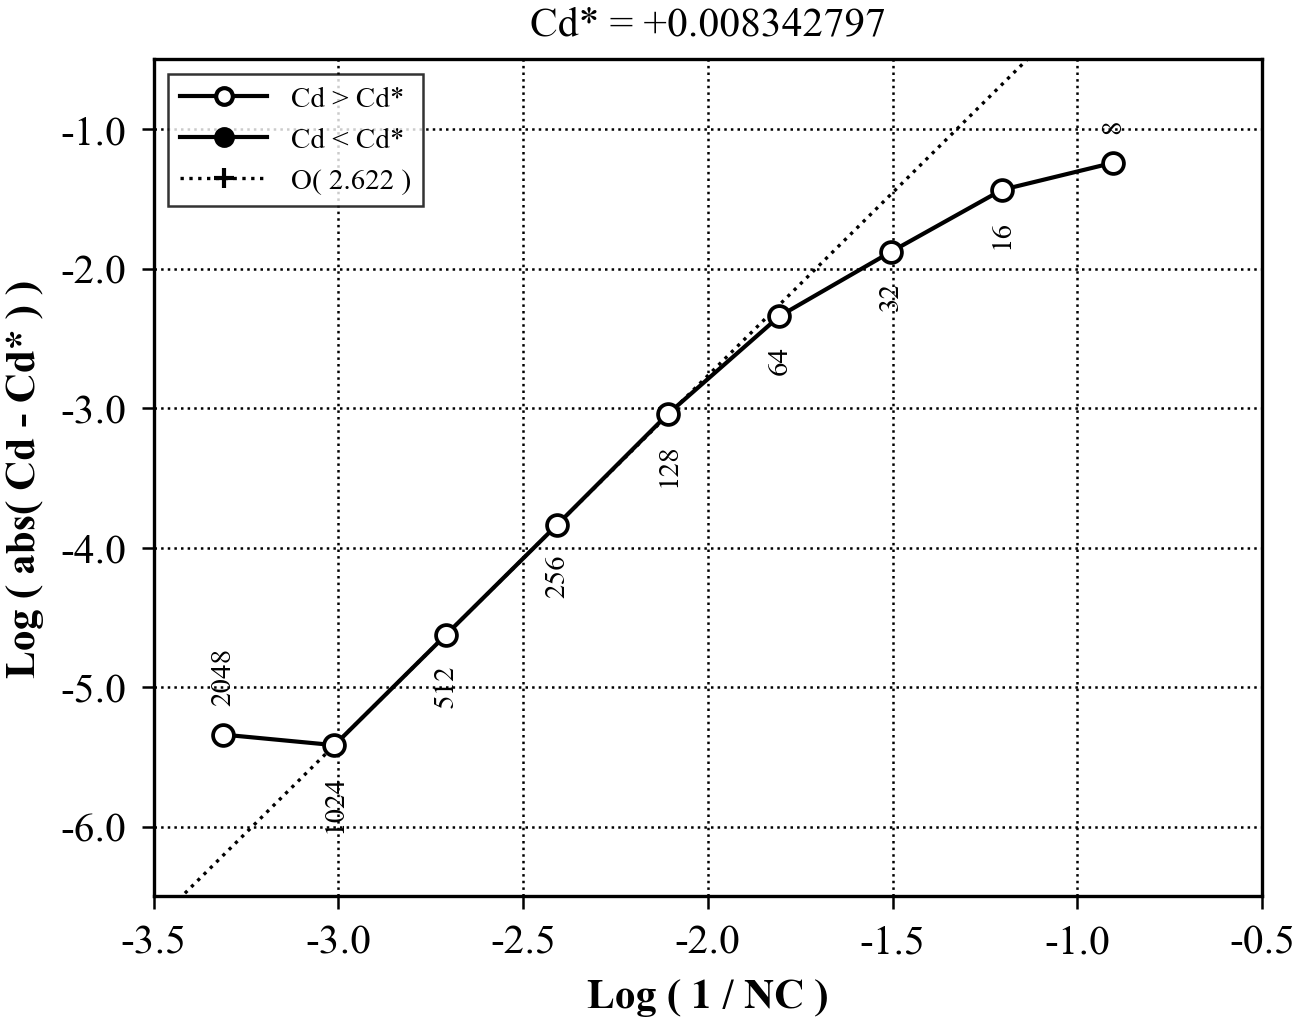
\includegraphics[width=\linewidth]{gc_M08HK_cd_a0.png}
    \caption{Drag, $\alpha=0^\circ$}
  \end{subfigure}\hfill
  \begin{subfigure}{0.48\linewidth}
    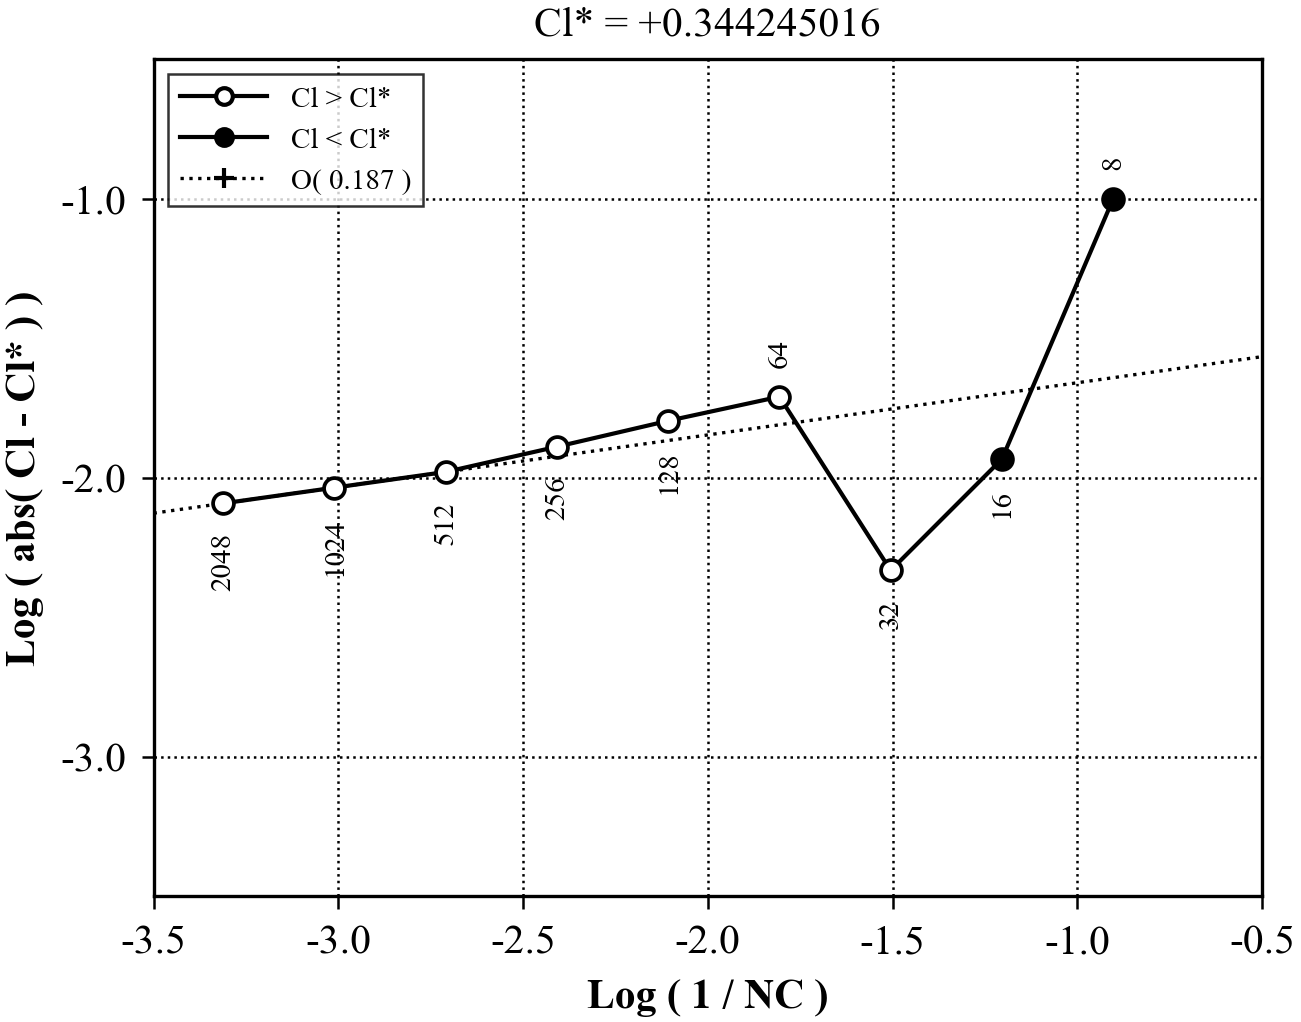
\includegraphics[width=\linewidth]{gc_M08HK_cl_a125.png}
    \caption{Lift, $\alpha=1.25^\circ$}
  \end{subfigure}\\[4pt]
  \begin{subfigure}{0.48\linewidth}
    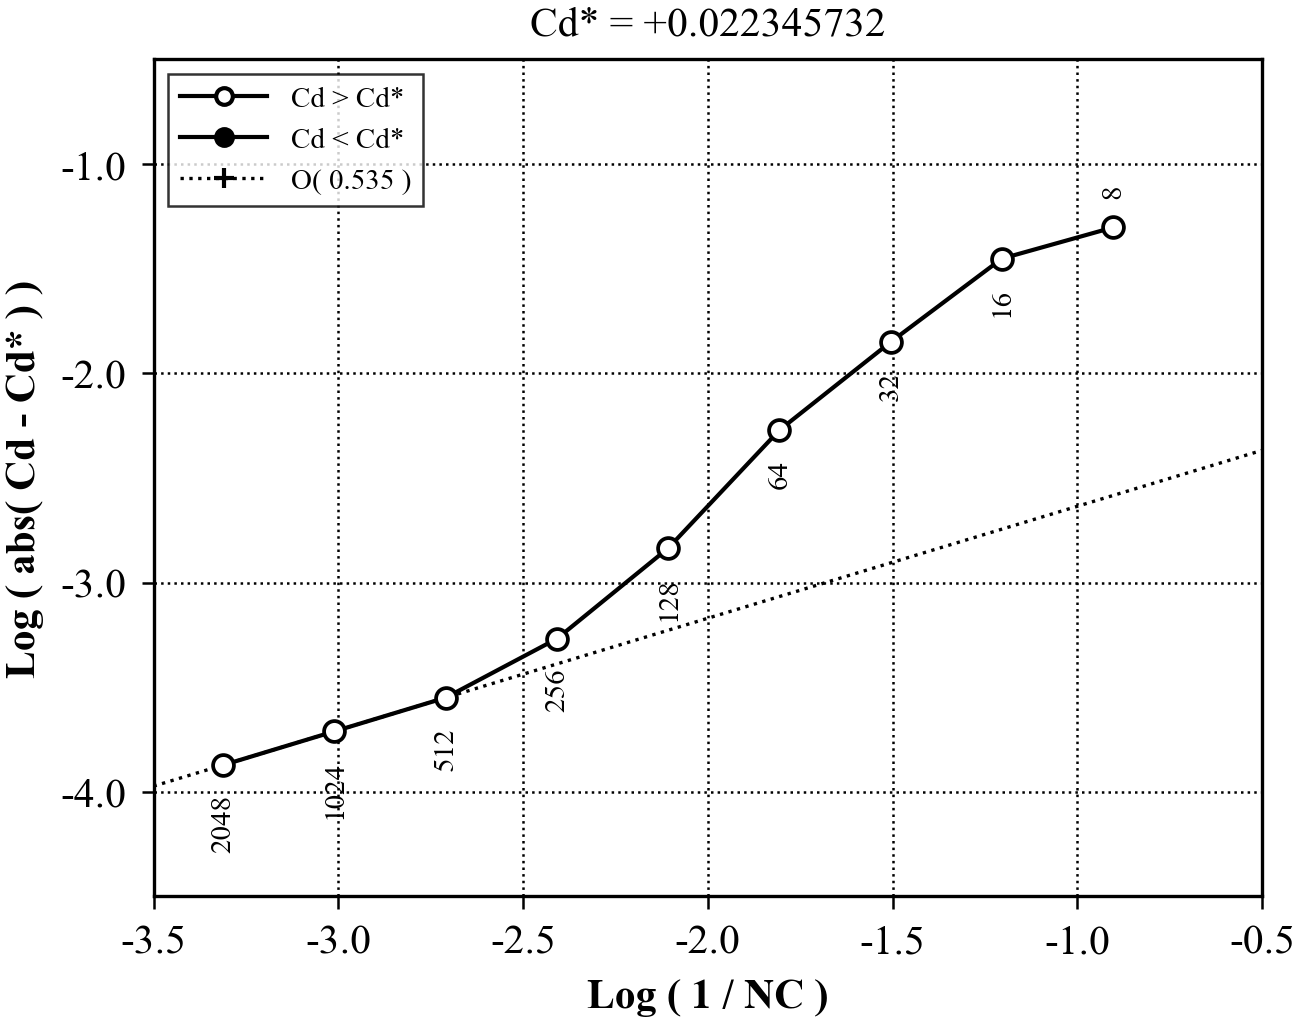
\includegraphics[width=\linewidth]{gc_M08HK_cd_a125.png}
    \caption{Drag, $\alpha=1.25^\circ$}
  \end{subfigure}\hfill
  \begin{subfigure}{0.48\linewidth}
    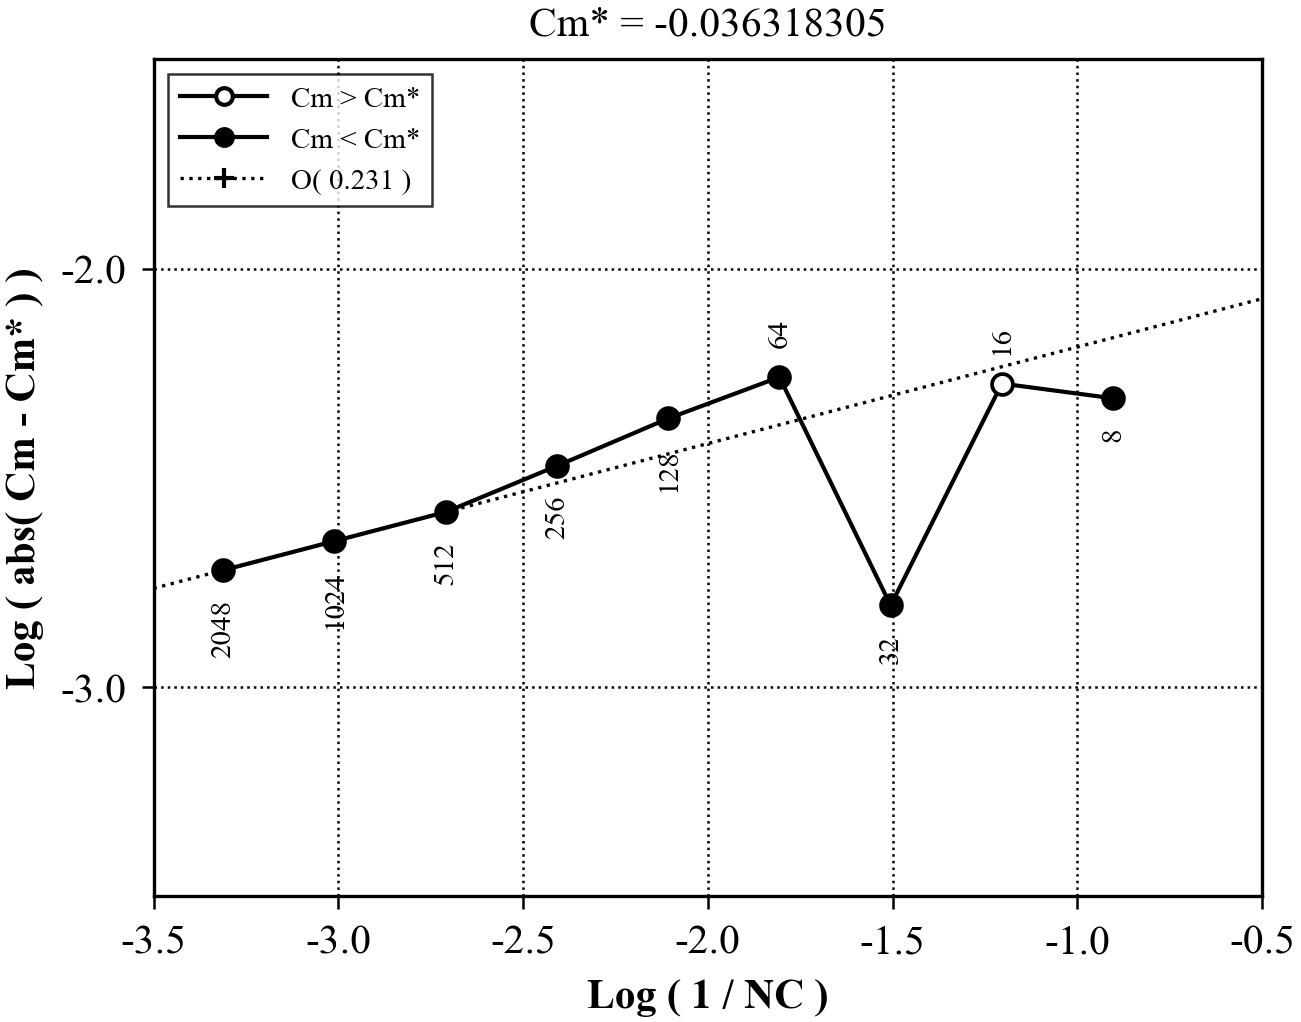
\includegraphics[width=\linewidth]{gc_M08HK_cm_a125.png}
    \caption{Moment, $\alpha=1.25^\circ$}
  \end{subfigure}
  \caption{Grid convergence of the force coefficients, $M_\infty=0.8$}
  \label{fig:gc_M08HK}
\end{figure}

\clearpage
\section{Grid convergence at \texorpdfstring{$M_\infty=0.8$}{M = 0.8}, Van Albada limiter}\label{app:gc_M08VA}

Table~\ref{tab:gc_M08VA} gives the observed order $p$ and the continuum value $F^*$ of the two finest
triplets (--: not monotone), and Figure~\ref{fig:gc_M08VA} the
convergence of the force coefficients on all grids. In the figures, open symbols mark $F>F^*$
and filled symbols $F<F^*$.

\begin{table}[H]
\centering
\caption{Observed order and continuum value, $M_\infty=0.8$, Van Albada limiter}
\label{tab:gc_M08VA}
\footnotesize
\setlength{\tabcolsep}{4pt}
\renewcommand{\arraystretch}{1.0}
\begin{tabular}{@{}llcccc@{}}
\toprule
 & & \multicolumn{2}{c}{$NC=256$, 512, 1024} & \multicolumn{2}{c}{$NC=512$, 1024, 2048} \\
\cmidrule(lr){3-4}\cmidrule(l){5-6}
$\alpha$ & $F$ & $p$ & $F^*$ & $p$ & $F^*$ \\
\midrule
$0^\circ$ & $C_D$ & 2.48 & $+0.008343138$ & 5.28 & $+0.008347021$ \\
$1.25^\circ$ & $C_L$ & 1.10 & $+0.352467906$ & 0.61 & $+0.351031243$ \\
 & $C_D$ & 1.57 & $+0.022504617$ & 0.91 & $+0.022444623$ \\
 & $C_M$ & 1.13 & $-0.038260938$ & 0.65 & $-0.037871161$ \\
\bottomrule
\end{tabular}
\end{table}

\begin{figure}[H]
  \centering
  \begin{subfigure}{0.48\linewidth}
    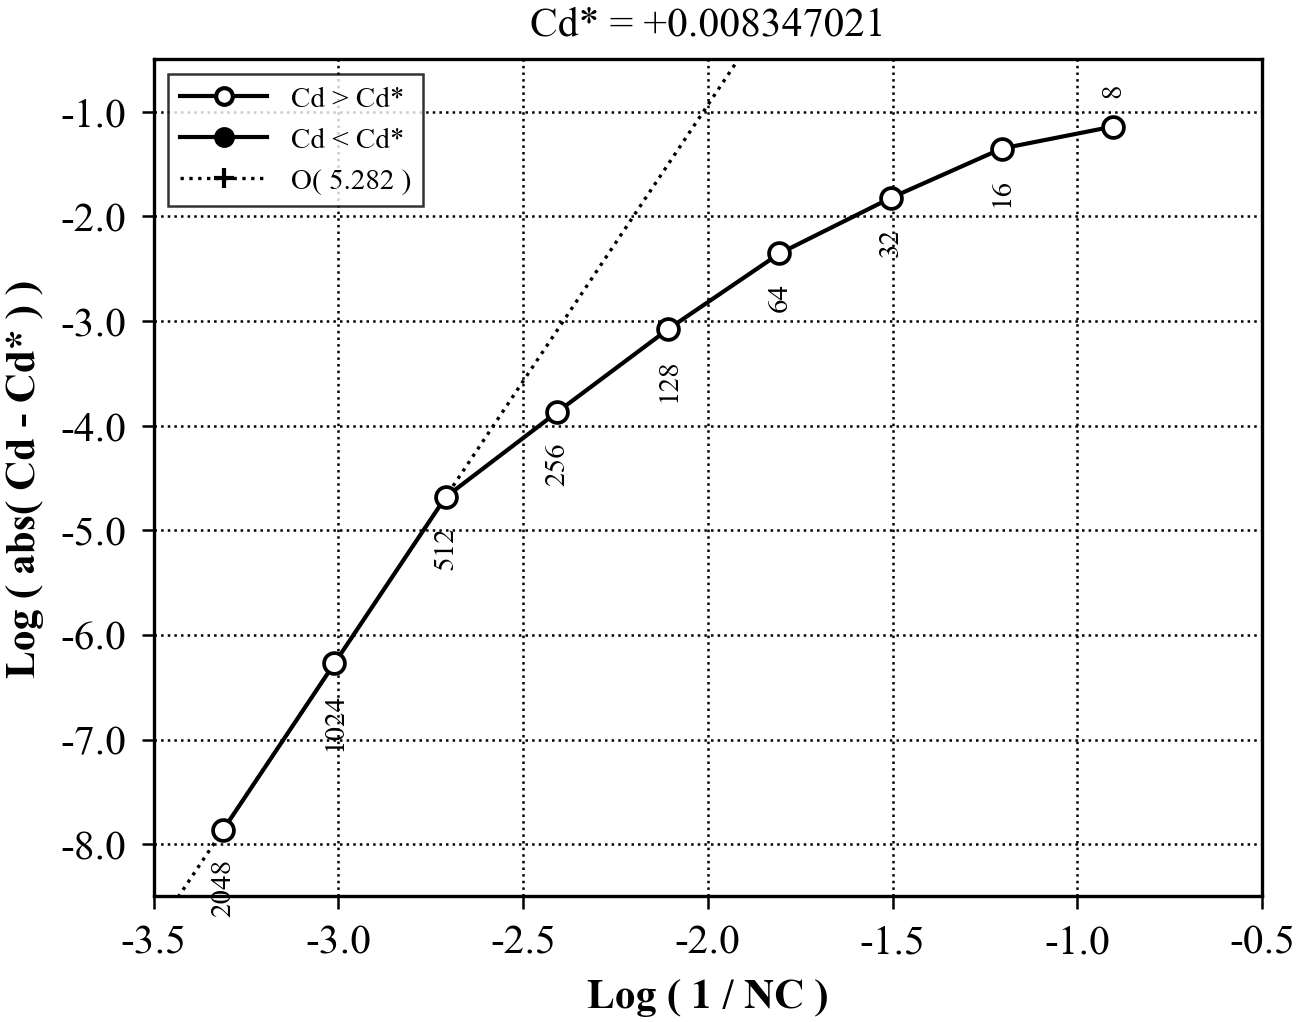
\includegraphics[width=\linewidth]{gc_M08VA_cd_a0.png}
    \caption{Drag, $\alpha=0^\circ$}
  \end{subfigure}\hfill
  \begin{subfigure}{0.48\linewidth}
    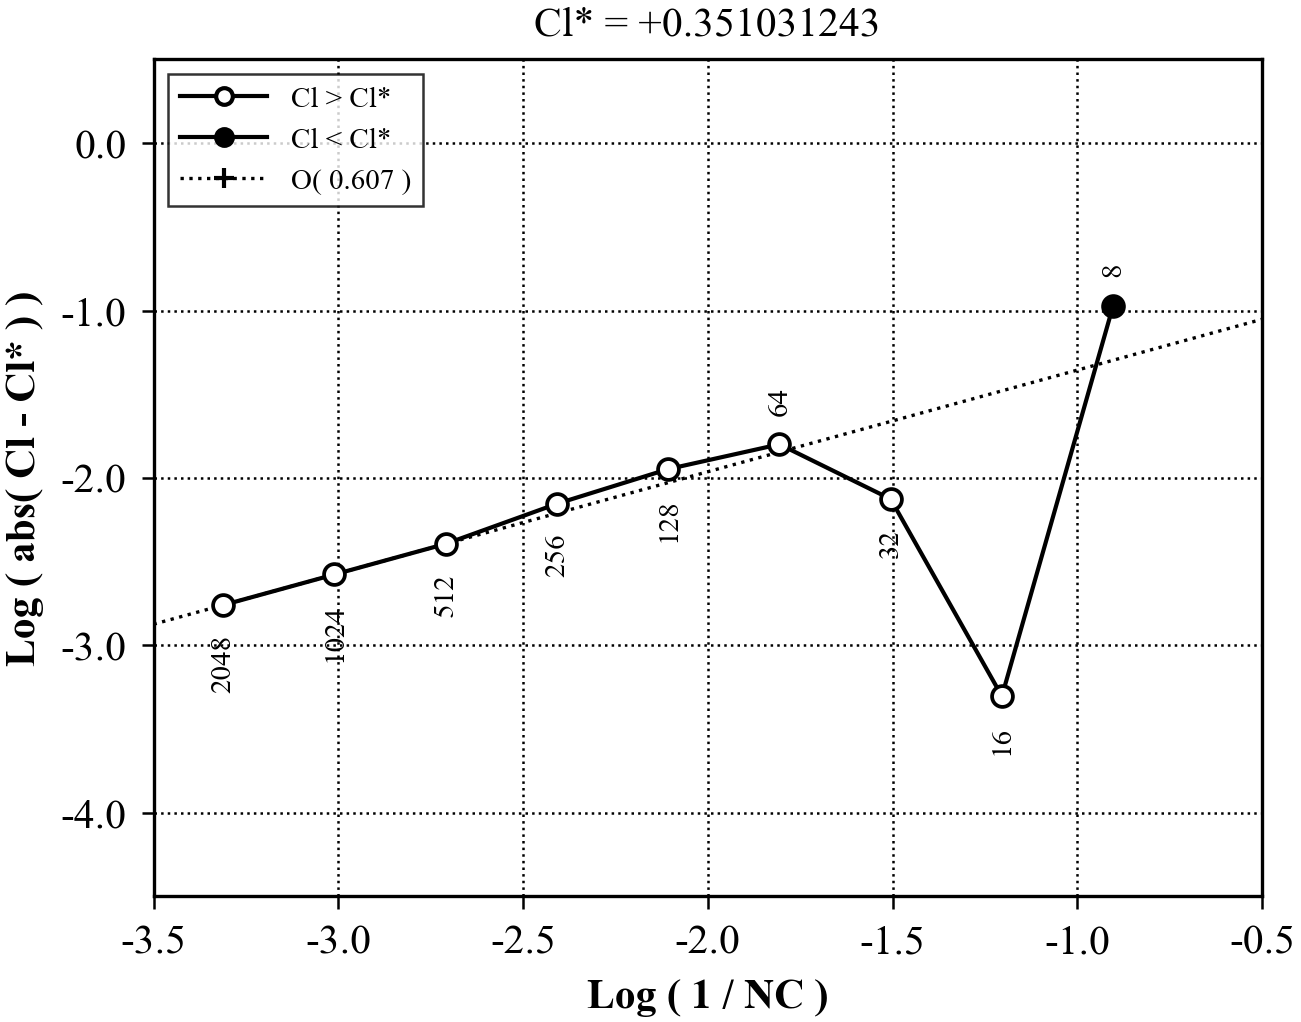
\includegraphics[width=\linewidth]{gc_M08VA_cl_a125.png}
    \caption{Lift, $\alpha=1.25^\circ$}
  \end{subfigure}\\[4pt]
  \begin{subfigure}{0.48\linewidth}
    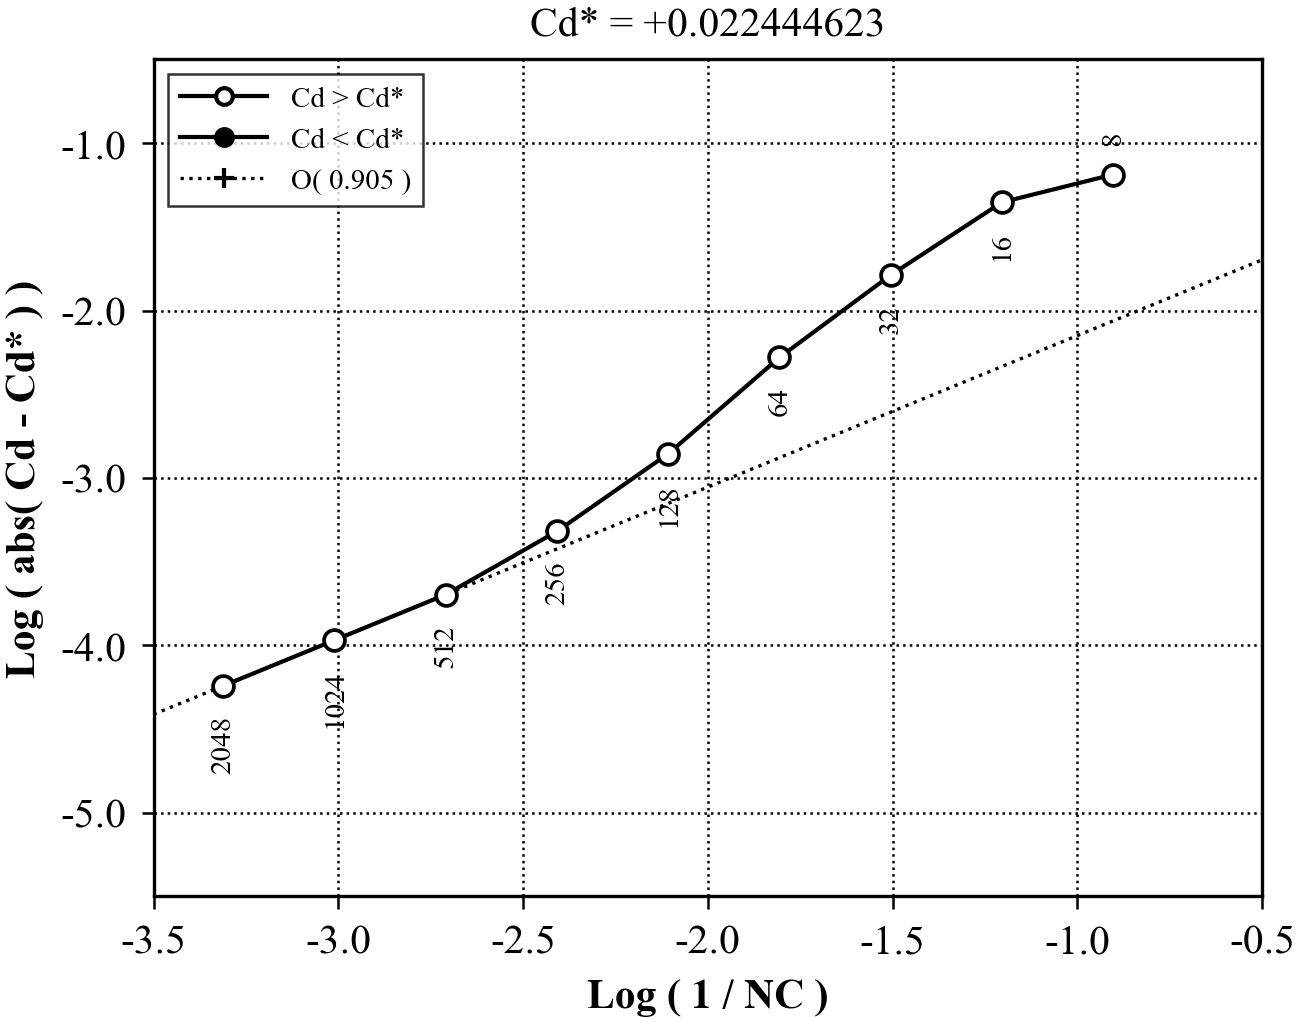
\includegraphics[width=\linewidth]{gc_M08VA_cd_a125.png}
    \caption{Drag, $\alpha=1.25^\circ$}
  \end{subfigure}\hfill
  \begin{subfigure}{0.48\linewidth}
    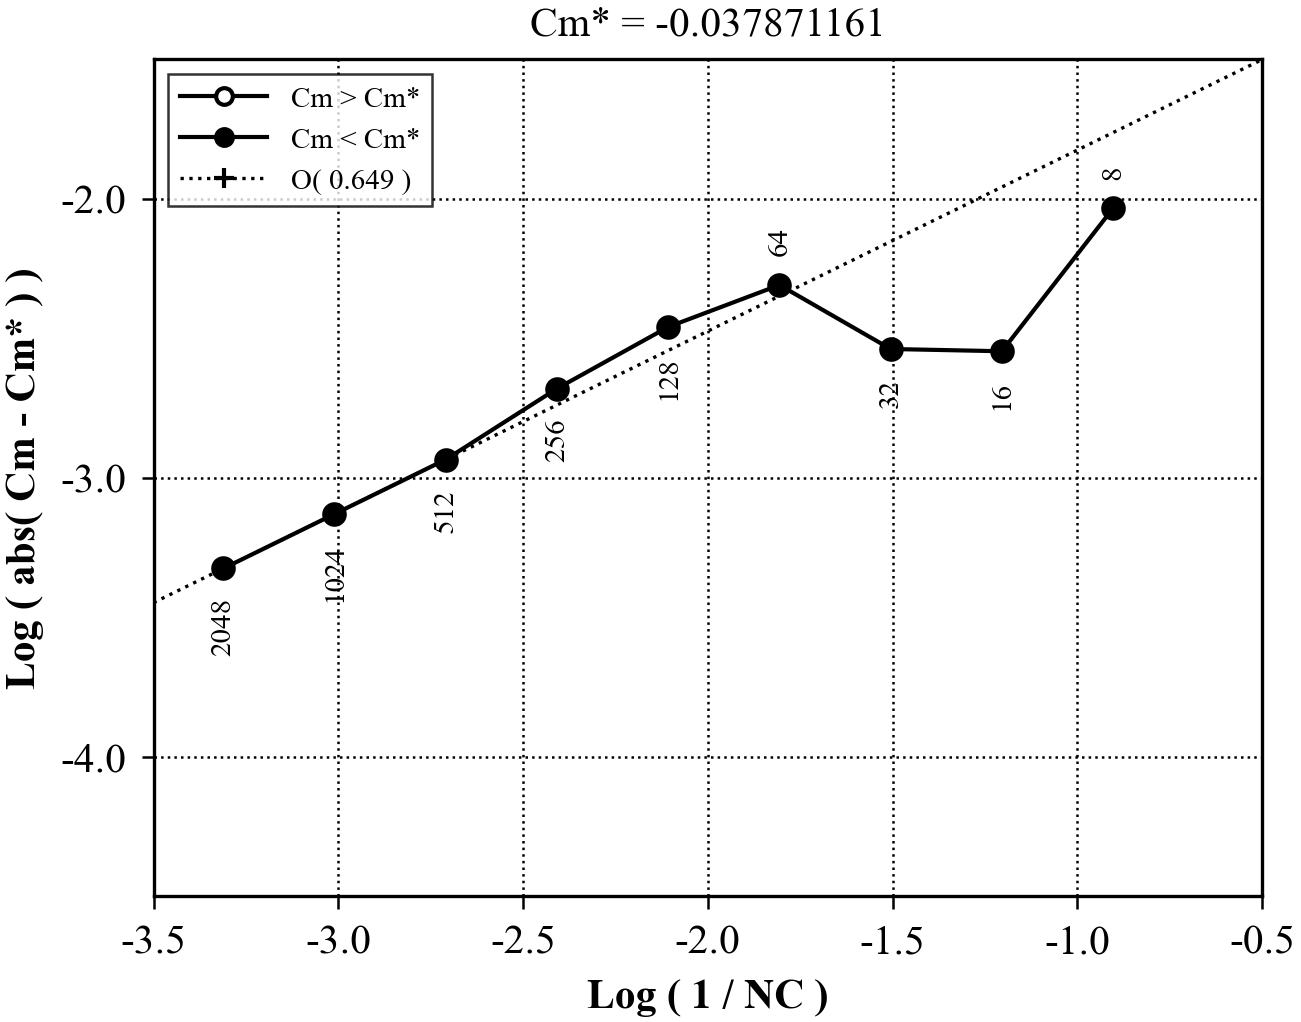
\includegraphics[width=\linewidth]{gc_M08VA_cm_a125.png}
    \caption{Moment, $\alpha=1.25^\circ$}
  \end{subfigure}
  \caption{Grid convergence of the force coefficients, $M_\infty=0.8$, Van Albada limiter}
  \label{fig:gc_M08VA}
\end{figure}

\clearpage
\section{Force coefficients with the Van Albada limiter}\label{app:va_forces}

Tables~\ref{tab:forces_M05VA} and~\ref{tab:forces_M08VA} give the force coefficients and run times
with the Van Albada limiter, in the format of Table~\ref{tab:gc_forces}.

\begin{table}[H]
\centering
\caption{Force coefficients and run times, $M_\infty=0.5$, Van Albada limiter}
\label{tab:forces_M05VA}
\footnotesize
\setlength{\tabcolsep}{4pt}
\renewcommand{\arraystretch}{1.0}
\begin{tabular}{@{}rrcrcccr@{}}
\toprule
\multicolumn{2}{c}{Mesh} & \multicolumn{2}{c}{$\alpha=0^\circ$} & \multicolumn{4}{c}{$\alpha=1.25^\circ$} \\
\cmidrule(lr){1-2}\cmidrule(lr){3-4}\cmidrule(l){5-8}
$NC$ & $NC^2$ & $C_D$ & $t$ (s) & $C_L$ & $C_D$ & $C_M$ & $t$ (s) \\
\midrule
8 & 64 & $+0.065469664$ & 0.02 & $+0.187219118$ & $+0.069128749$ & $-0.014320409$ & 0.01 \\
16 & 256 & $+0.043590326$ & 0.02 & $+0.171312753$ & $+0.045220137$ & $-0.005094853$ & 0.02 \\
32 & 1{,}024 & $+0.020794137$ & 0.06 & $+0.166681012$ & $+0.022143059$ & $-0.002778758$ & 0.05 \\
64 & 4{,}096 & $+0.007077552$ & 0.26 & $+0.176240334$ & $+0.006718971$ & $-0.002315246$ & 0.33 \\
128 & 16{,}384 & $+0.001429635$ & 2.32 & $+0.178026991$ & $+0.001437813$ & $-0.002132188$ & 2.92 \\
256 & 65{,}536 & $+0.000233787$ & 19.8 & $+0.179124097$ & $+0.000256478$ & $-0.002225346$ & 22.9 \\
512 & 262{,}144 & $+0.000036880$ & 190.9 & $+0.179321179$ & $+0.000058010$ & $-0.002246508$ & 206.2 \\
1{,}024 & 1{,}048{,}576 & $+0.000006546$ & 1{,}862 & $+0.179361486$ & $+0.000027332$ & $-0.002251978$ & 2{,}450 \\
2{,}048 & 4{,}194{,}304 & $+0.000002722$ & 15{,}500 & $+0.179368147$ & $+0.000023559$ & $-0.002253008$ & 17{,}462 \\
\bottomrule
\end{tabular}
\end{table}

\begin{table}[H]
\centering
\caption{Force coefficients and run times, $M_\infty=0.8$, Van Albada limiter}
\label{tab:forces_M08VA}
\footnotesize
\setlength{\tabcolsep}{4pt}
\renewcommand{\arraystretch}{1.0}
\begin{tabular}{@{}rrcrcccr@{}}
\toprule
\multicolumn{2}{c}{Mesh} & \multicolumn{2}{c}{$\alpha=0^\circ$} & \multicolumn{4}{c}{$\alpha=1.25^\circ$} \\
\cmidrule(lr){1-2}\cmidrule(lr){3-4}\cmidrule(l){5-8}
$NC$ & $NC^2$ & $C_D$ & $t$ (s) & $C_L$ & $C_D$ & $C_M$ & $t$ (s) \\
\midrule
8 & 64 & $+0.080668366$ & 0.02 & $+0.244150929$ & $+0.087441495$ & $-0.047138390$ & 0.01 \\
16 & 256 & $+0.052908931$ & 0.17 & $+0.351528200$ & $+0.066790010$ & $-0.040717048$ & 0.03 \\
32 & 1{,}024 & $+0.023346831$ & 0.07 & $+0.358513306$ & $+0.038734746$ & $-0.040770548$ & 0.10 \\
64 & 4{,}096 & $+0.012768405$ & 0.55 & $+0.366918432$ & $+0.027689874$ & $-0.042787864$ & 15.6 \\
128 & 16{,}384 & $+0.009183991$ & 4.26 & $+0.362330249$ & $+0.023839585$ & $-0.041348586$ & 17.0 \\
256 & 65{,}536 & $+0.008481310$ & 24.2 & $+0.358045340$ & $+0.022924771$ & $-0.039961784$ & 66.6 \\
512 & 262{,}144 & $+0.008367847$ & 205.7 & $+0.355072069$ & $+0.022645741$ & $-0.039035777$ & 306.7 \\
1{,}024 & 1{,}048{,}576 & $+0.008347556$ & 2{,}106 & $+0.353683817$ & $+0.022552019$ & $-0.038613924$ & 2{,}814 \\
2{,}048 & 4{,}194{,}304 & $+0.008347035$ & 40{,}745 & $+0.352772508$ & $+0.022501972$ & $-0.038344877$ & 65{,}106 \\
\bottomrule
\end{tabular}
\end{table}

\clearpage
\section{Convergence monitoring}\label{app:conv}

Figures~\ref{fig:conv_M05} to~\ref{fig:conv_M125} show the convergence of the cases of
Section~\ref{sec:flows} at $\alpha=1.25^\circ$, and Figure~\ref{fig:conv_M08CL} that of the fixed-lift
case of Section~\ref{sec:fixedcl}: the density residual drop on every grid from $129\times129$, and
the convergence of $C_L$, $C_D$ and $C_M$ to their final value on the finest grid. Grids
$257\times257$ and finer start from the FMG solution (Appendix~\ref{app:fmg}).

\begin{figure}[H]
  \centering
  \begin{subfigure}[t]{0.49\linewidth}
    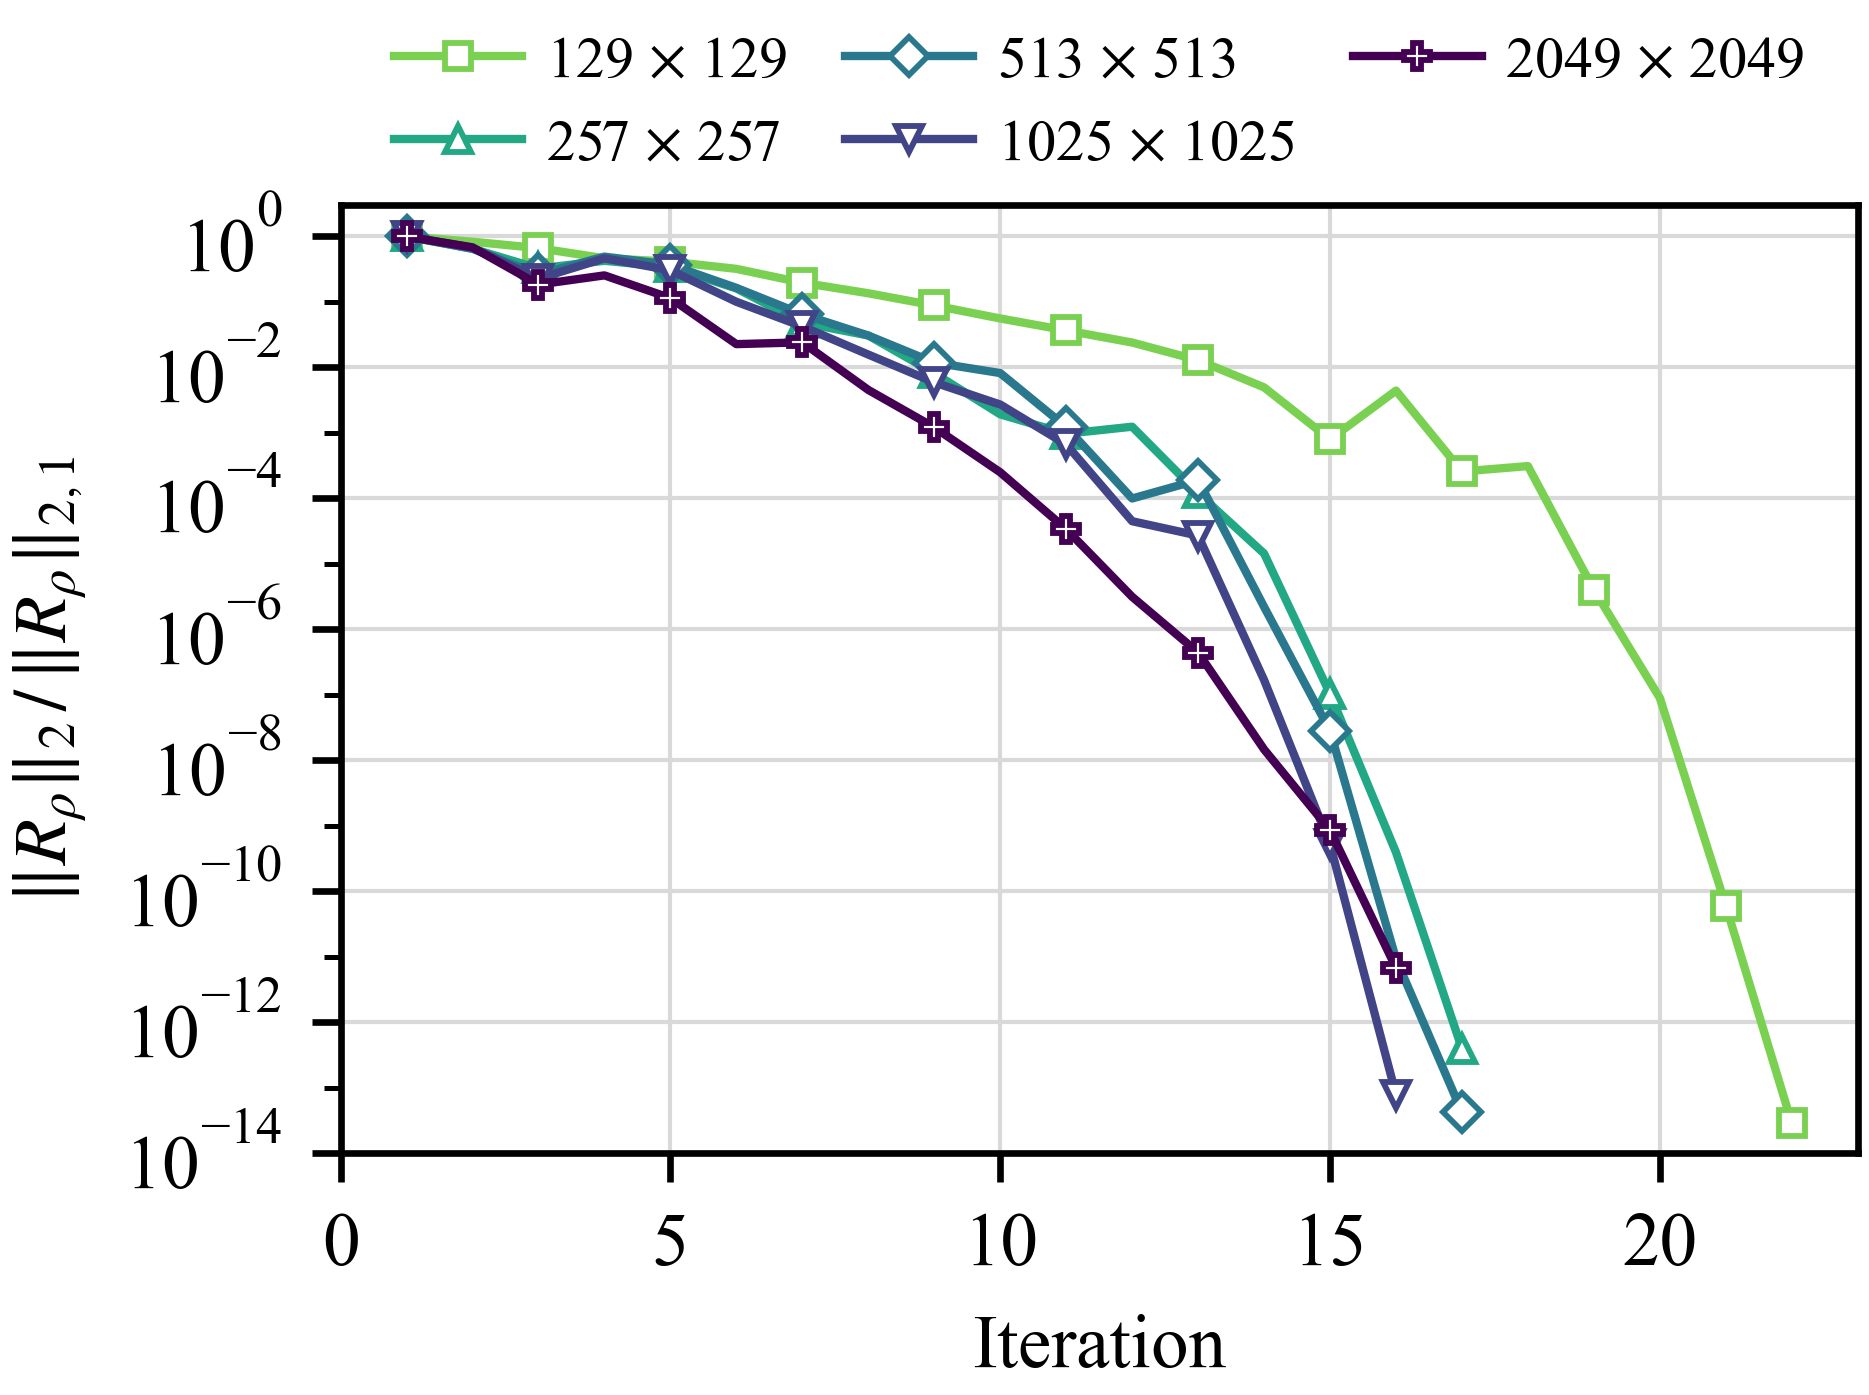
\includegraphics[width=\linewidth]{conv_M05_a125.png}
    \caption{Density residual}
  \end{subfigure}\hfill
  \begin{subfigure}[t]{0.49\linewidth}
    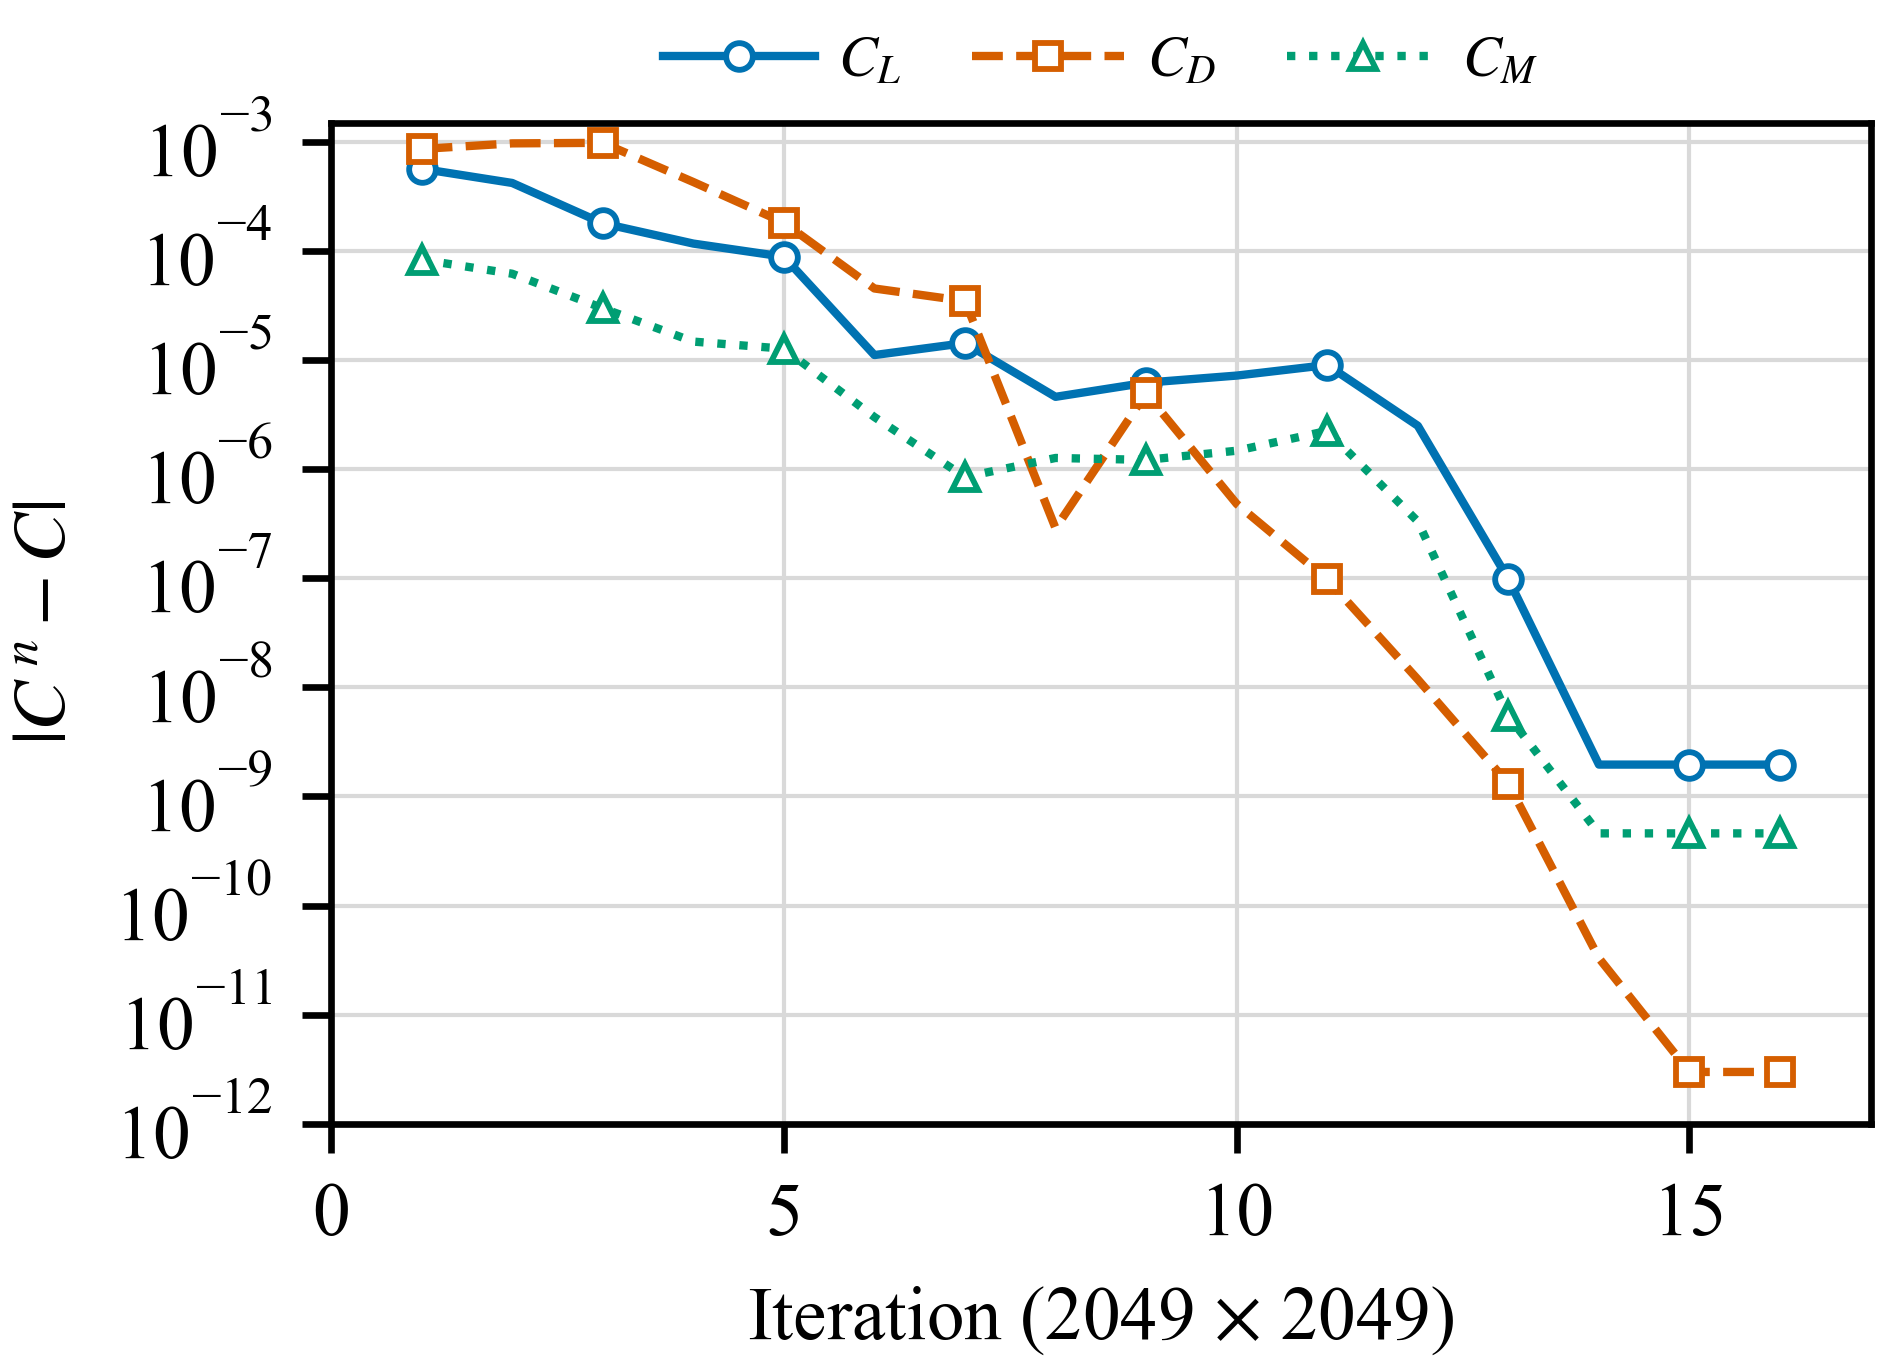
\includegraphics[width=\linewidth]{conv_forces_M05_a125.png}
    \caption{Force coefficients}
  \end{subfigure}
  \caption{Convergence, $M_\infty=0.5$, $\alpha=1.25^\circ$}
  \label{fig:conv_M05}
\end{figure}

\begin{figure}[H]
  \centering
  \begin{subfigure}[t]{0.49\linewidth}
    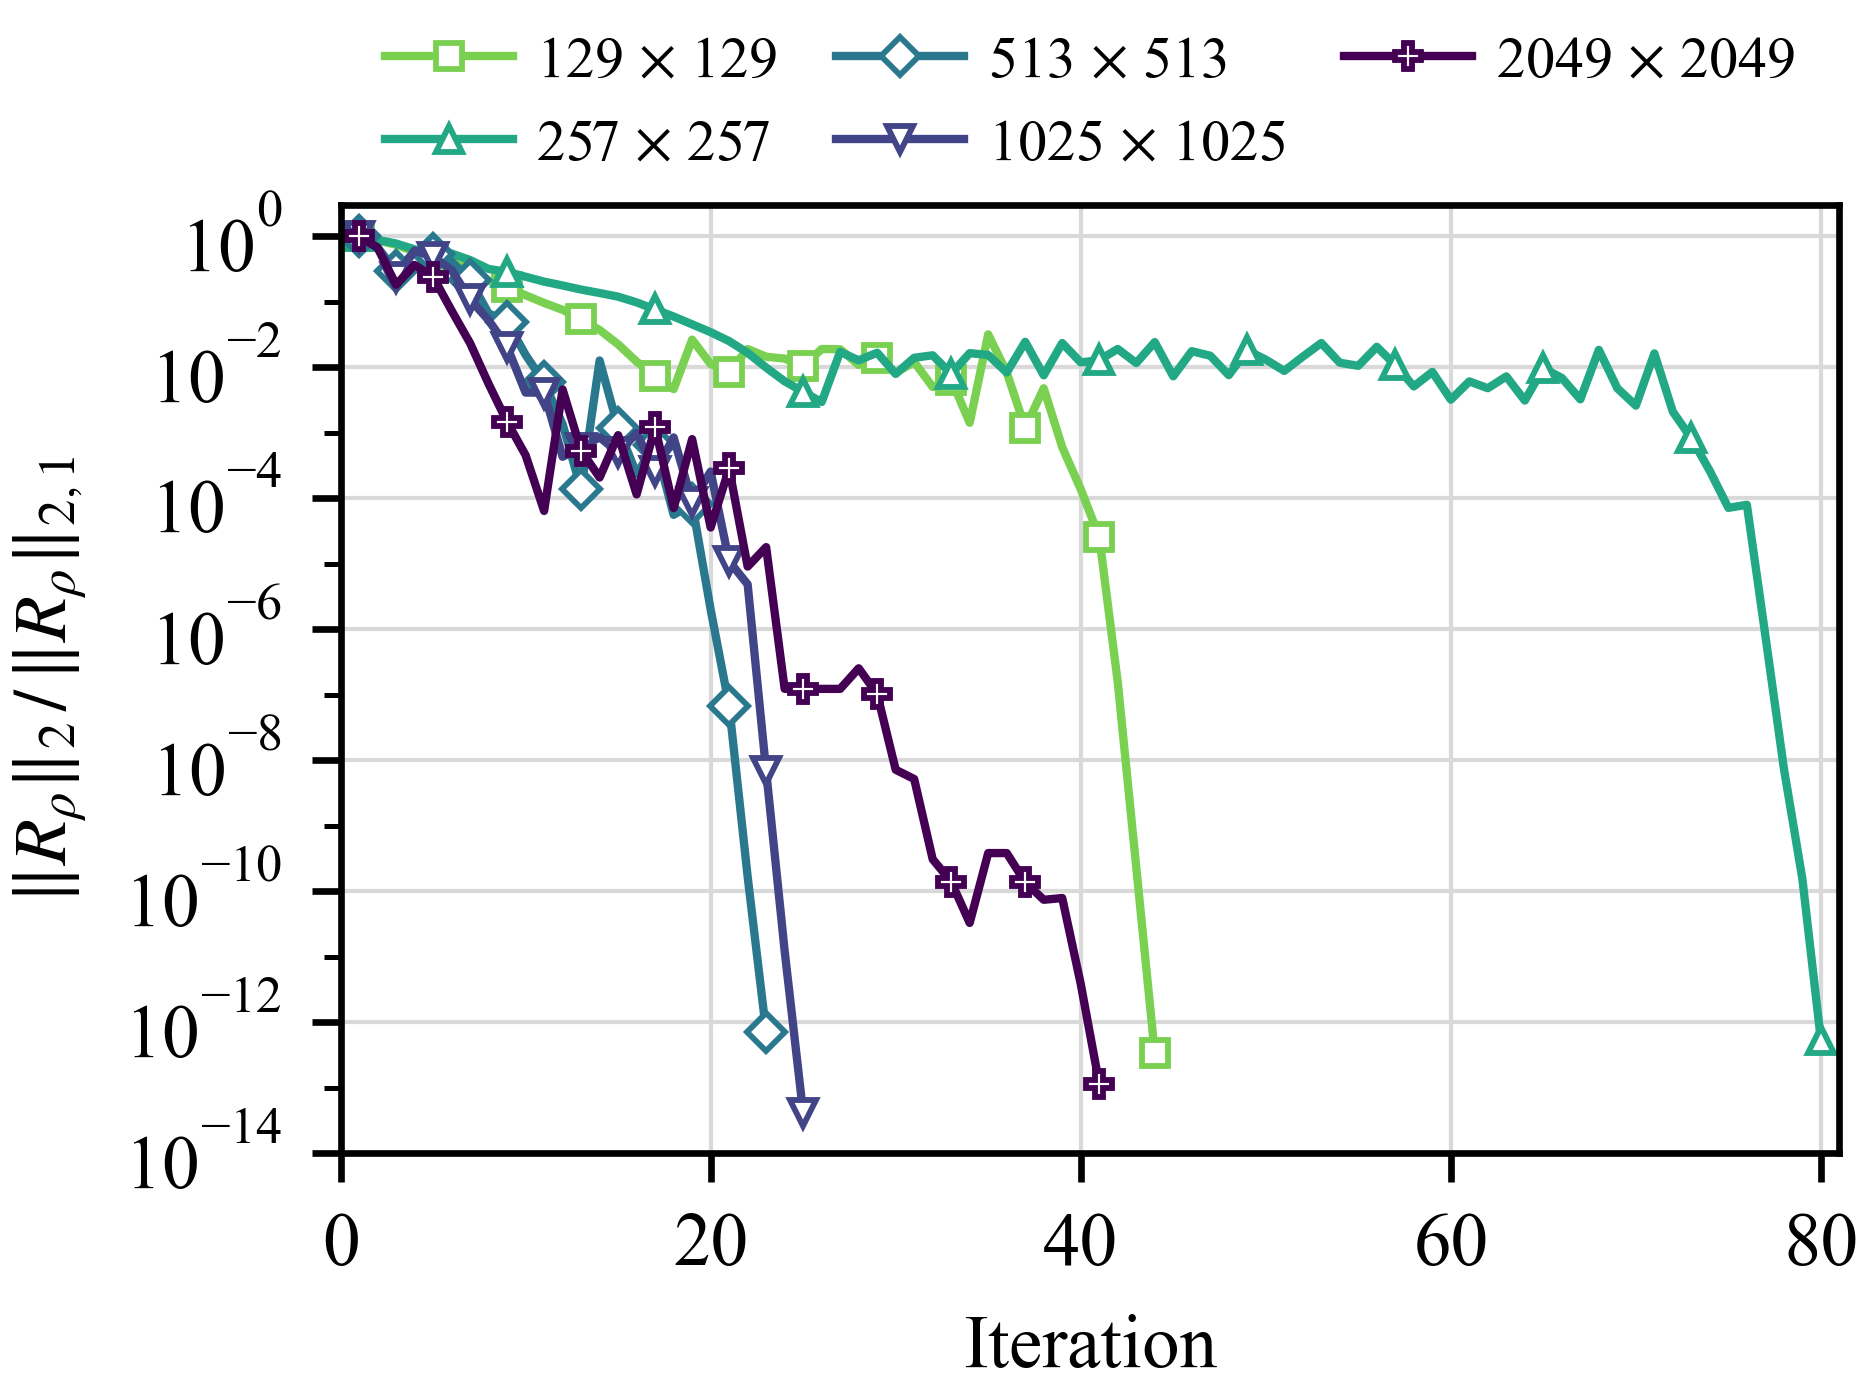
\includegraphics[width=\linewidth]{conv_M08_a125.png}
    \caption{Density residual}
  \end{subfigure}\hfill
  \begin{subfigure}[t]{0.49\linewidth}
    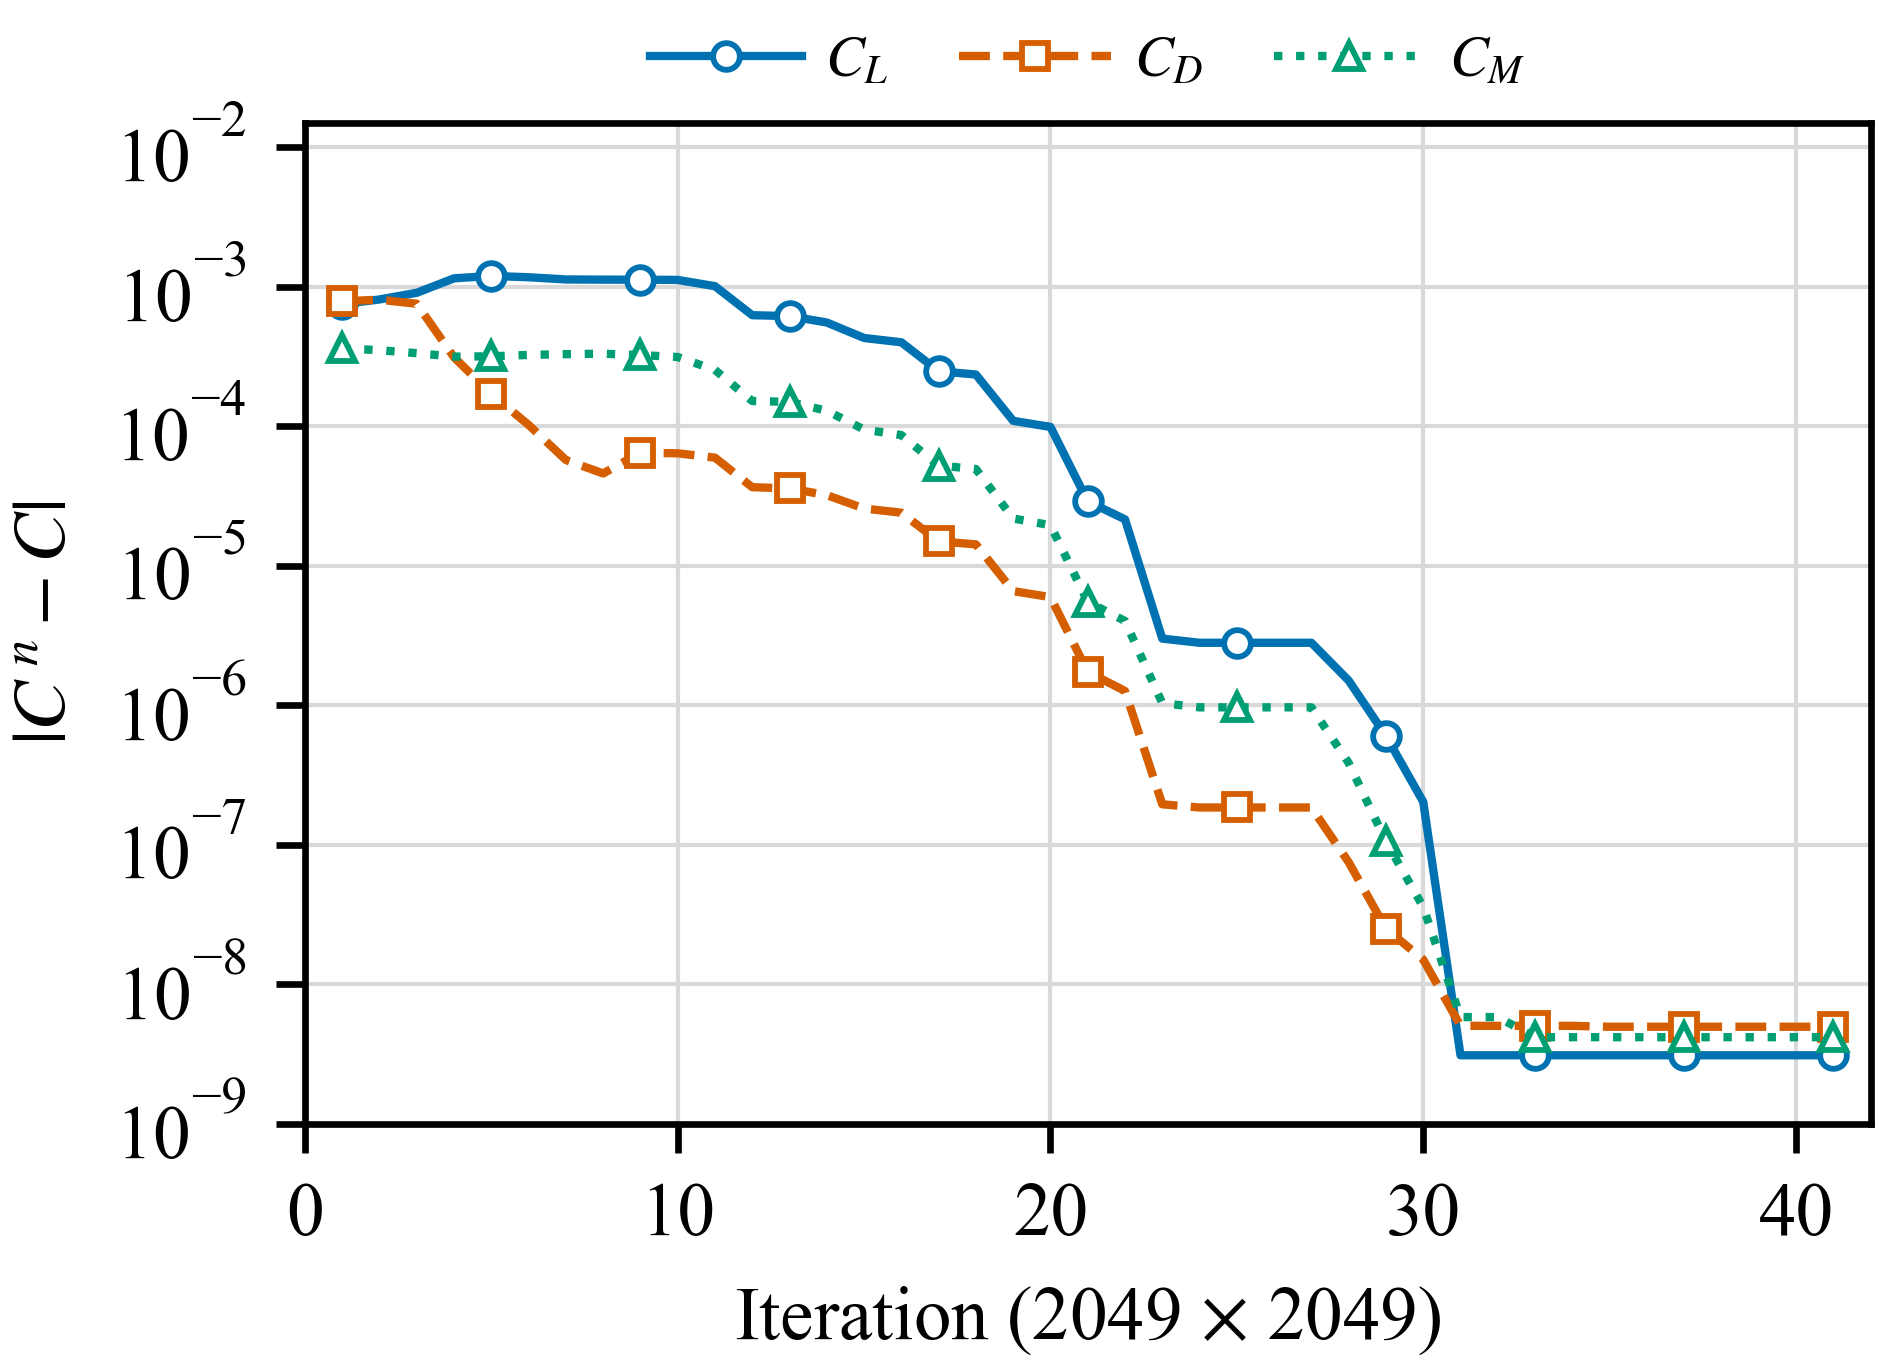
\includegraphics[width=\linewidth]{conv_forces_M08_a125.png}
    \caption{Force coefficients}
  \end{subfigure}
  \caption{Convergence, $M_\infty=0.8$, $\alpha=1.25^\circ$}
  \label{fig:conv_M08}
\end{figure}

\begin{figure}[H]
  \centering
  \begin{subfigure}[t]{0.49\linewidth}
    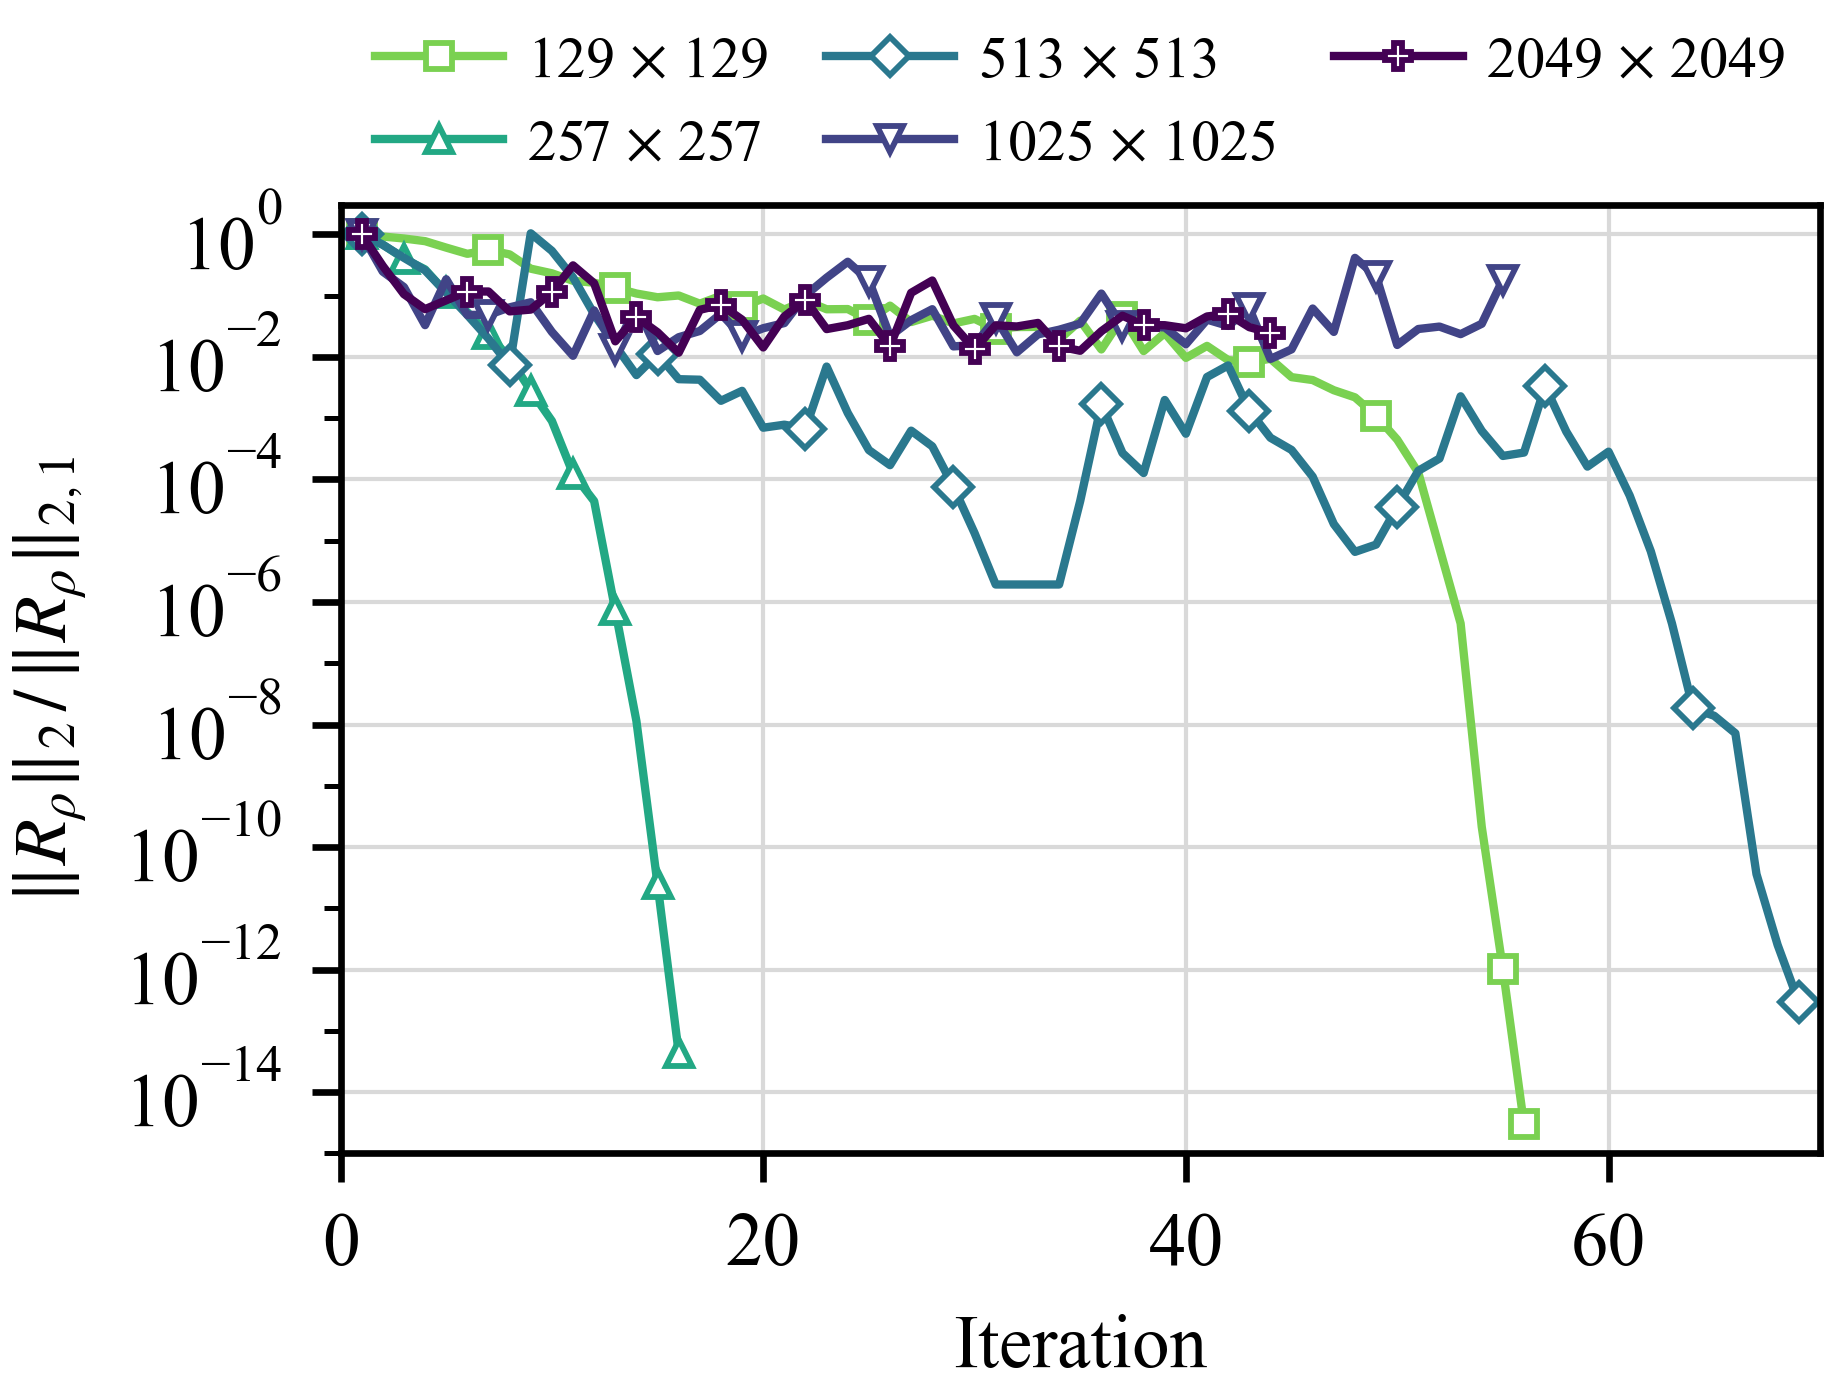
\includegraphics[width=\linewidth]{conv_M125_a125.png}
    \caption{Density residual}
  \end{subfigure}\hfill
  \begin{subfigure}[t]{0.49\linewidth}
    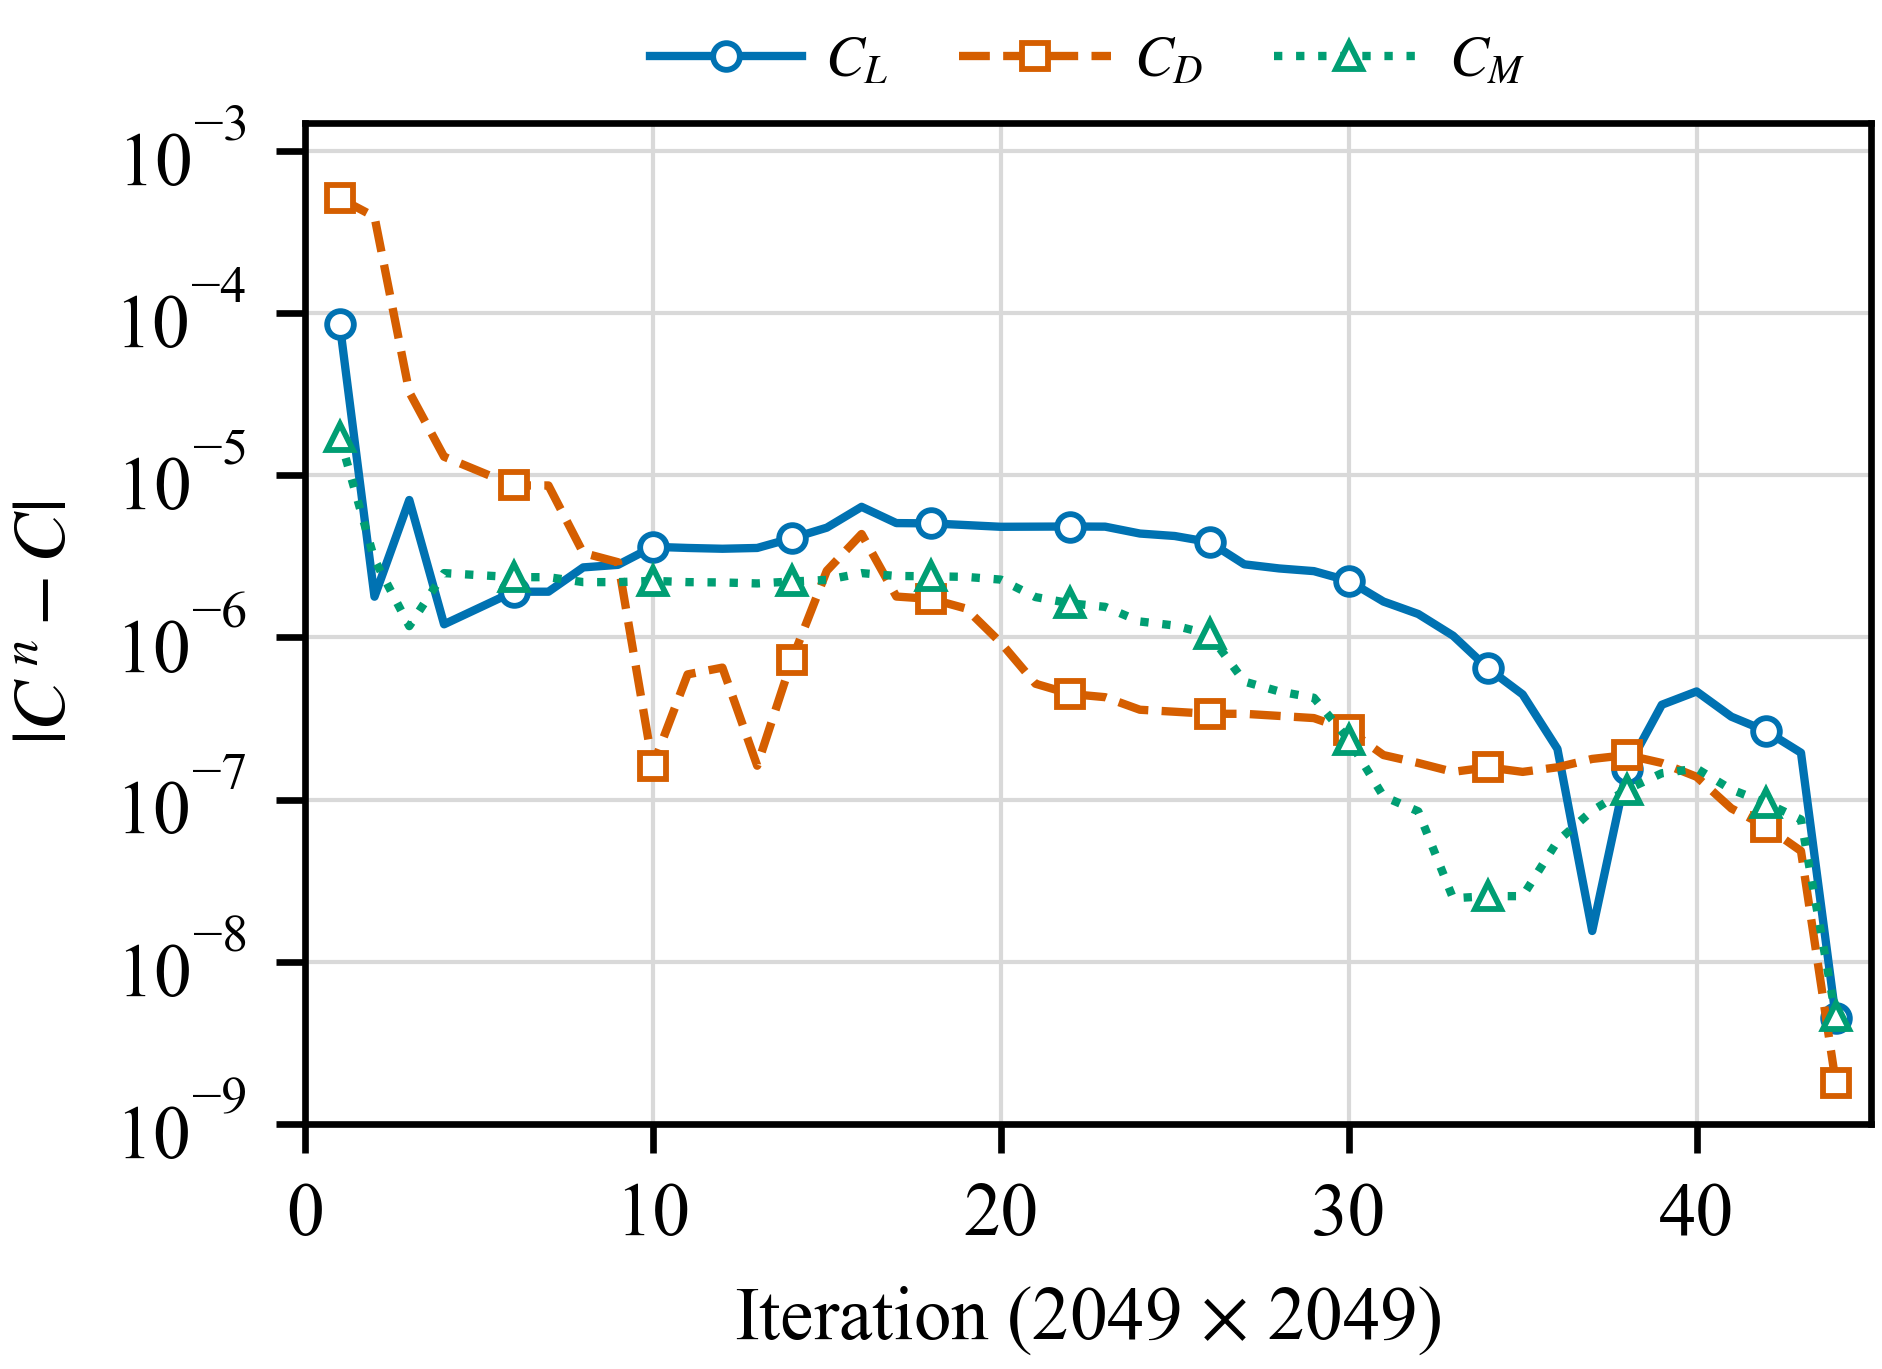
\includegraphics[width=\linewidth]{conv_forces_M125_a125.png}
    \caption{Force coefficients}
  \end{subfigure}
  \caption{Convergence, $M_\infty=1.25$, $\alpha=1.25^\circ$}
  \label{fig:conv_M125}
\end{figure}

\begin{figure}[H]
  \centering
  \begin{subfigure}[t]{0.49\linewidth}
    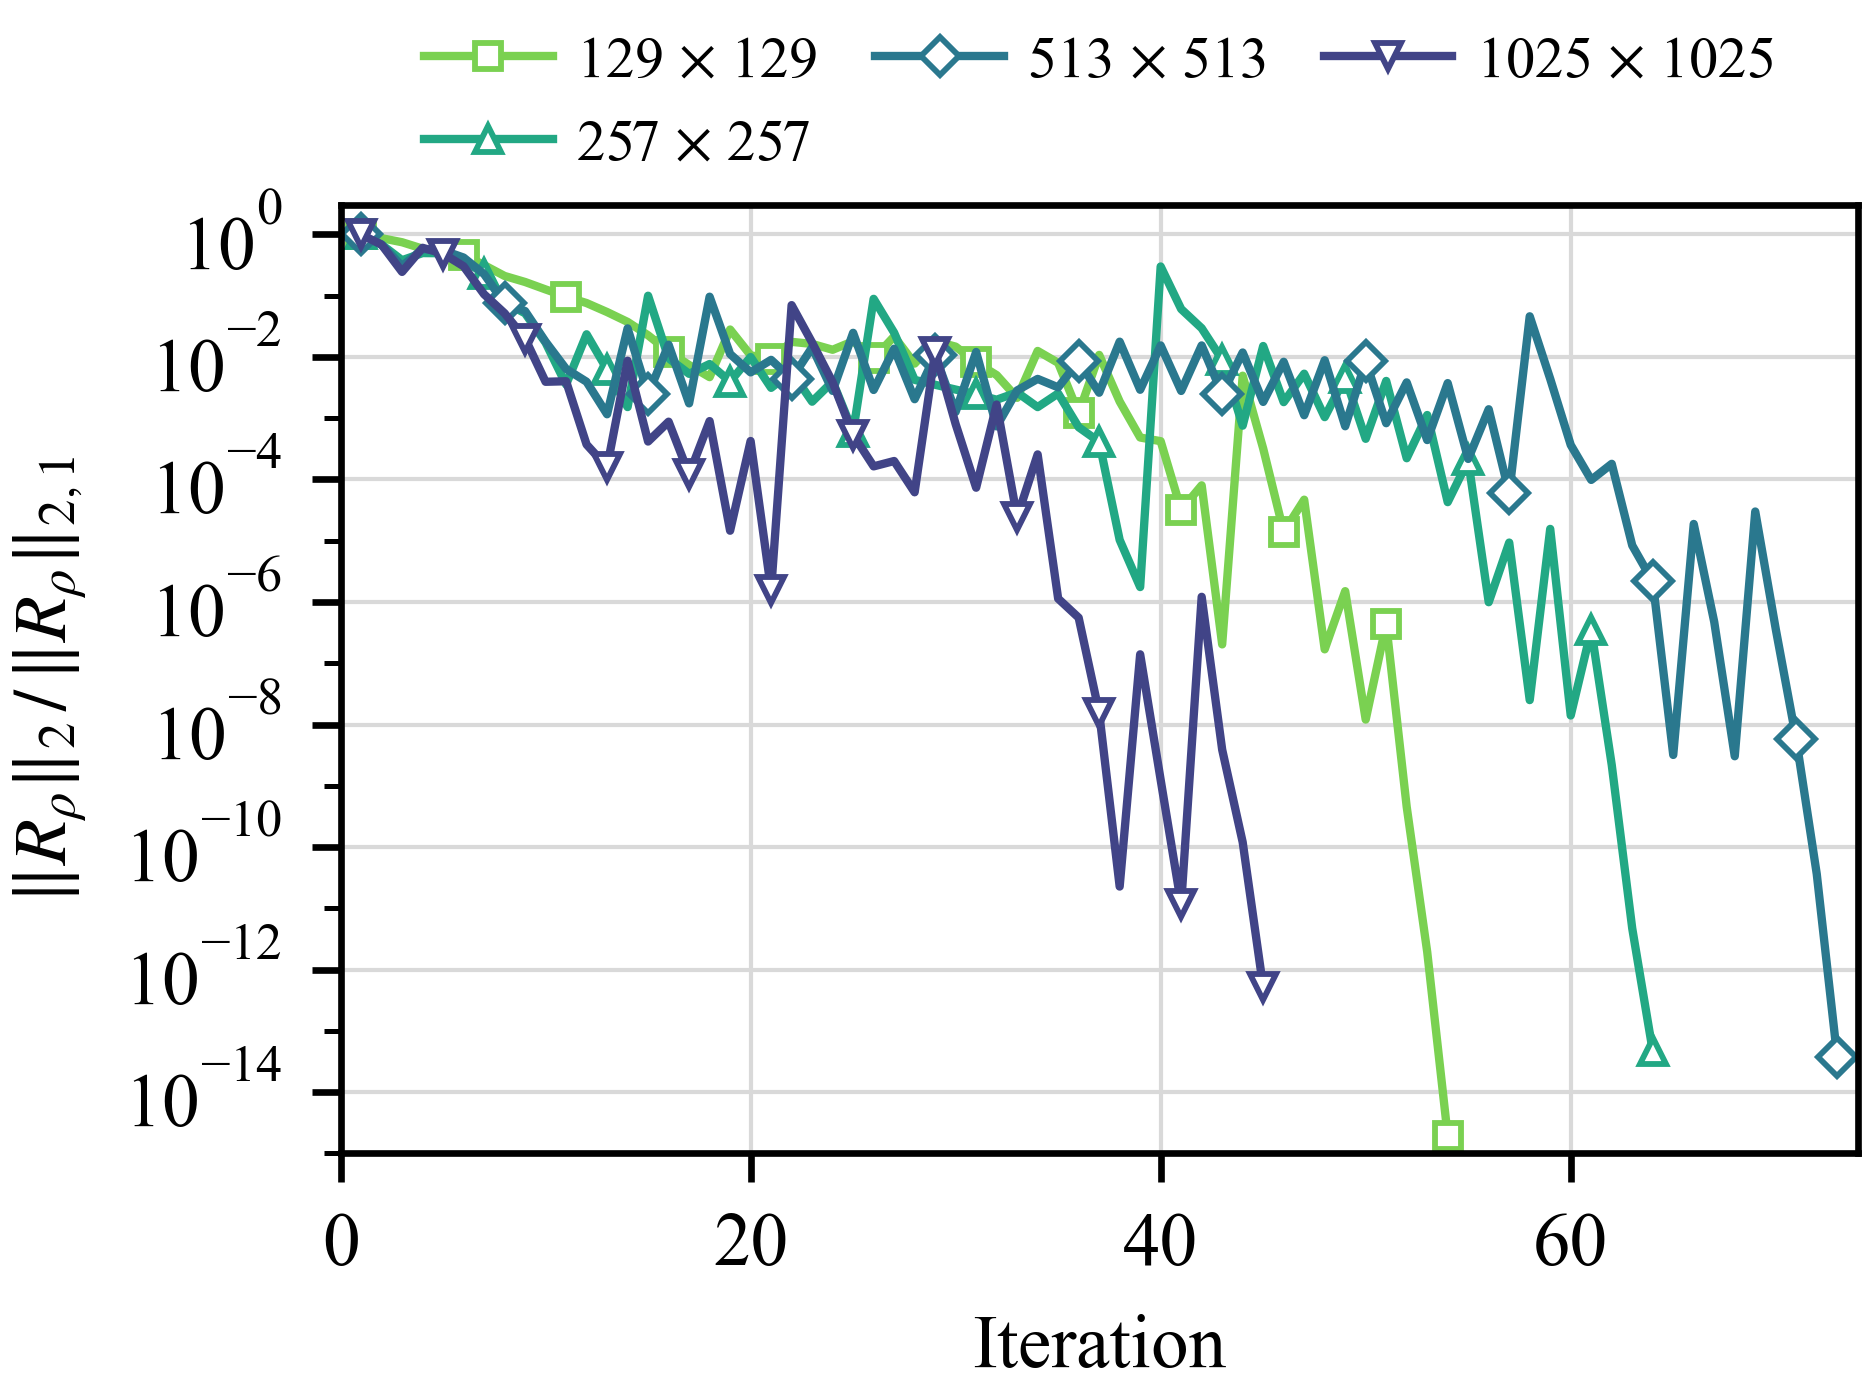
\includegraphics[width=\linewidth]{conv_M08_CL04.png}
    \caption{Density residual}
  \end{subfigure}\hfill
  \begin{subfigure}[t]{0.49\linewidth}
    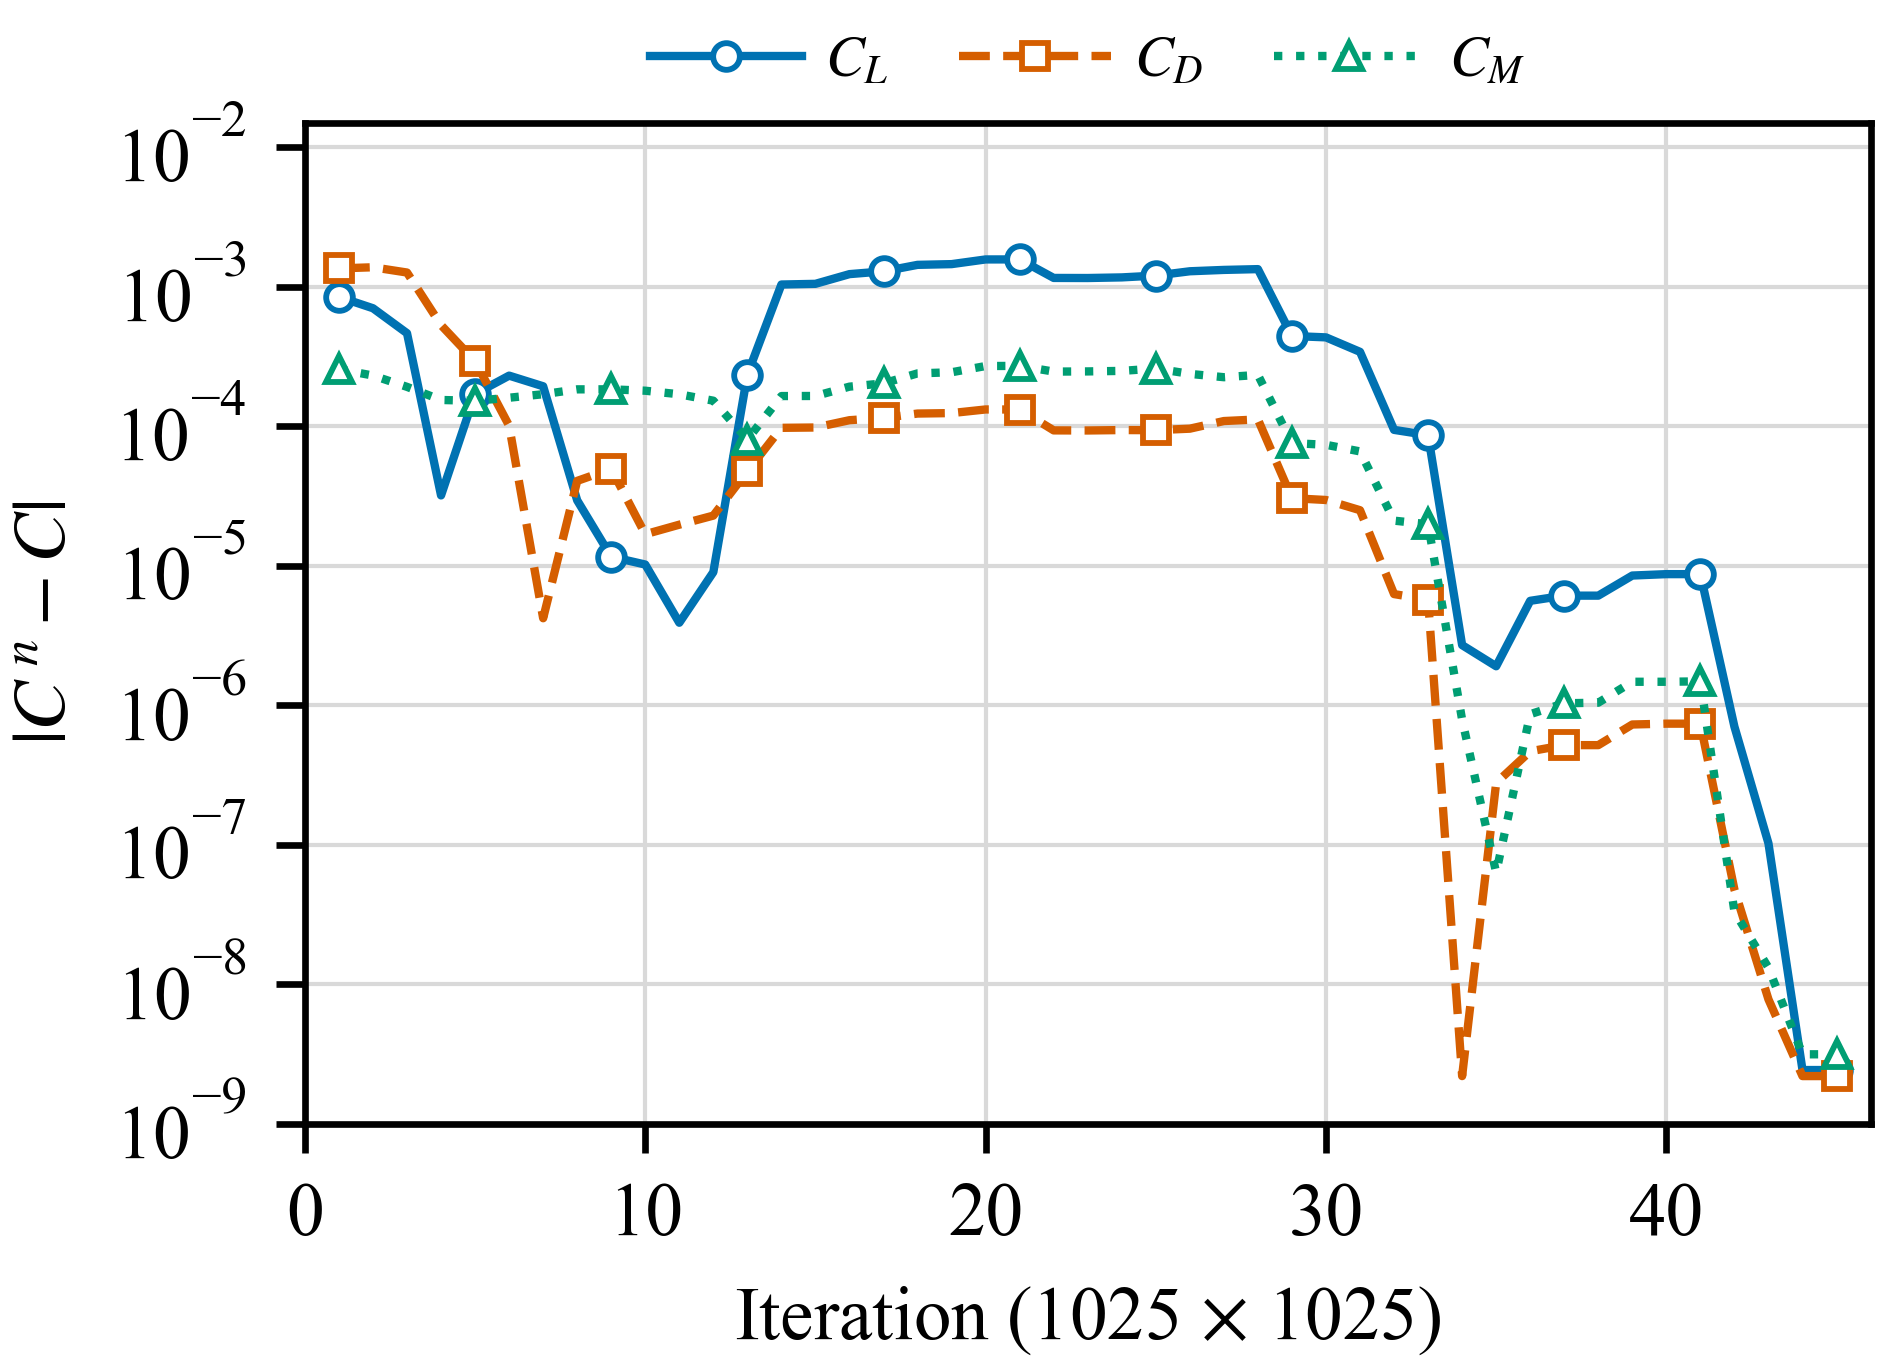
\includegraphics[width=\linewidth]{conv_forces_M08_CL04.png}
    \caption{Force coefficients}
  \end{subfigure}
  \caption{Convergence, $M_\infty=0.8$, $C_L=0.4$}
  \label{fig:conv_M08CL}
\end{figure}

\end{document}
